\chapter{Introduction}
Clouds are a ubiquitous part of the atmosphere and can have a significant impact on many Earth-atmosphere processes \citep{rog1989,lamb2011,mur2012,tan2016,milt2018-2}. These impacts, and the processes that lead to the formation of clouds in the first place, are areas of atmospheric science that are still full of uncertainties due to the complex, small-scale interactions that are involved \citep{ipcc5,mcfa2017,milt2018-2}. The goal of the project covered by this thesis was to investigate one of those areas of uncertainty: cloud ice formation. Specifically, the goal was to determine what ice formation processes were active in mixed-phase stratus clouds observed over Antarctica. The method of choice for this project was to use model simulations based on cloud and environment observations to evaluate what processes and environmental characteristics were required to produce the cloud ice distribution patterns that were observed in the Antarctic clouds.

\section{Scope}
This thesis focuses on cloud ice production processes and numerical modeling of cloud microphysics. Background knowledge is provided for the following topics: aerosol characteristics and processes, cloud droplet formation, ice nucleation, secondary ice production, Antarctic clouds and climate, and atmospheric modeling. Details are provided about the development, structure, and configuration of the Met Office NERC Cloud (MONC) model and the Cloud AeroSol Interactions Microphysics (CASIM) scheme with specific focus on mixed-phase cloud simulations.

\section{Structure of Thesis}
Chapter \ref{ch:cloudPhys} provides an overview of cloud physics topics and the relevance of the field of study to atmospheric science as a whole. Section \ref{ch:aero} covers details on the types and characteristics of atmospheric aerosols and the cloud physics processes they are involved in. Section \ref{ch:act} covers details of cloud droplet formation processes and parameterizations for including those processes in numerical models. Section \ref{ch:iceNuc} covers details on ice nucleation processes and parameterizations for including those processes in numerical models. Section \ref{ch:sip} covers details on secondary ice production processes and parameterizations for including those processes in numerical models. Section \ref{ch:ant} provides an overview of Antarctic clouds and climate and their significance to atmospheric science research. Section \ref{ch:mac} provides an overview of the Microphysics of Antarctic Clouds (MAC) field campaign, including the instruments used and the environmental characteristics observed during the campaign. Chapter \ref{ch:mac} also provides a comparison between the Antarctic and the Arctic. Chapter \ref{ch:modeling} introduces cloud physics modeling, including an overview of the history and development of atmospheric models (\ref{sec:modeling}), model types (\ref{sec:modelCats} - \ref{sec:schemeTypes}), the current state of modeling (\ref{sec:currentState}), and an introduction to the models used in this project (\ref{sec:projectModels}). Section \ref{ch:monc} provides details on the Met Office NERC Cloud (MONC) model. Section \ref{ch:casim} provides details on the Cloud AeroSol Interactions Microphysics (CASIM) scheme. Section \ref{ch:moncConfig} goes into details on how to configure MONC, including an overview of the default configuration settings and guidance on some of the user-defined settings. Section \ref{ch:build} describes the process of building and running MONC. Section \ref{ch:processing} explains how the model output data is formatted and how to process the data. This section also includes some general troubleshooting techniques and common error messages with a description of what they mean and how to fix them. Section \ref{ch:method} provides an overview of the initial research question for the project, the challenges faced, and the choice of thesis topic and structure. Section \ref{ch:reality} provides details on how the project was tackled and what methods were used. Sections \ref{sec:profile} - \ref{sec:running} provide details on how model runs were produced. Section \ref{sec:results} provides examples of some of the model output data and a discussion on how it compares to the observations. Chapter \ref{ch:discussion} discusses the main findings of this project as well as providing an overview of future work that could benefit from the content of this thesis, including example research questions and potential directions for model development. Chapter \ref{ch:conclusion} concludes this thesis.

\section{Note on Model Code References}
Throughout this thesis there are times when the MONC and CASIM model code is referenced directly. When the code is explicitly referenced the relevant file from the model will be cited along with an indicator of whether it is a MONC or CASIM file. All model code is available through the Met Office Science Repository Service. Access to the MONC and CASIM repositories can be requested through the Met Office Science Partnerships department.

\chapter{Overview of Cloud Physics} \label{ch:cloudPhys}
\section{Cloud Physics Research and Relevance}
Clouds play a critical role in the atmosphere and impact numerous aspects of the Earth-atmosphere system both locally and globally from regulating daily temperature values, to producing precipitation, to influencing global circulation patterns, to complex climate change interactions. Clouds are a ubiquitous, though still relatively poorly understood, aspect of the Earth-atmosphere system \citep{mur2012,ipcc5,mcfa2017,milt2018-2}. Two of the reasons for this limited understanding are the challenges of collecting in-situ cloud measurements and the vast complexity of cloud systems and the processes and interactions within them. Despite these challenges, a fuller understanding of clouds and cloud processes is critical for a fuller understanding of other aspects of the atmosphere and, in turn, for weather and climate forecasting.

The complexity of clouds and their interconnection with other aspects of the Earth-atmosphere system means that cloud physics covers a wide range of topics. Regardless of the specific research question being explored, there are some foundational topics that are needed, at least to some degree, for almost any sort of cloud physics research. Those foundational topics are outlined in the following section and then will be described more fully in the next chapter. After the overview of the foundational topics is an introduction to some of the impacts clouds and cloud physics research have on other branches of atmospheric science as well as an overview of cloud physics research methods.

\section{Foundational Topics in Cloud Physics}
Within the vast area of topics that are covered in cloud physics, there are three topics that are foundational to understanding cloud lifecycles and processes. Those topics are: aerosol processes, cloud droplet formation and growth, and ice crystal formation and growth. Most research questions in cloud physics will require some understanding of these topics.

\subsection{Aerosol Characteristics and Processes}
Although it is possible in some environments for cloud particles to form homogeneously using only pure water, generally other substances are involved in the form of aerosol particles \citep{rog1989,lamb2011}. Aerosols are liquid and solid particles that are suspended in a gas. In atmospheric science, cloud particles (i.e. cloud drops, ice crystals, snow, graupel, and rain) are treated separately and are referred to as hydrometeors even though technically they too are types of aerosols. \citep{bouc2015} There are many types of atmospheric aerosols including: condensed gases, mineral powders and dusts, bioaerosols, combustion aerosols, and volcanic ash. 

Aerosols impact many aspects of the Earth-atmosphere system such as the radiation budget and climate change, air quality and pollution, and water cycle chemistry \citep{bouc2015}. The focus of this thesis is aerosol impacts on cloud formation. Regarding cloud formation, aerosols can be sorted into two categories: cloud condensation nuclei (CCN) and ice nucleating particles (INP). CCN are particles that can act as condensation surfaces for the formation of liquid cloud drops from ambient water vapour \citep{rog1989,bouc2015}. INPs are particles that can trigger heterogeneous ice nucleation \citep{vali2015}. Aerosols and aerosol processes will be covered in detail in Section \ref{ch:aero}.

\subsection{Cloud Droplet Formation and Growth}
Clouds are composed of water particles in the form of liquid drops, ice crystals, or both. Even when studying ice clouds, it is important to understand liquid drop formation and growth because water generally passes through the liquid phase before ice forms. Liquid drops can form from water vapour through either homogeneous or heterogeneous nucleation. Homogeneous nucleation involves only pure water molecules. Heterogeneous nucleation involves the addition of aerosol particles which allow condensation at a lower supersaturation than required for homogeneous nucleation \citep{rog1989,lamb2011}. Homogeneous nucleation is generally not considered a cloud formation process because it requires supersaturation values that are higher than typically observed in the atmosphere. Cloud drop nucleation and the parameterizations used to simulate such processes are covered in detail in Section \ref{ch:act}. 

Once liquid drops form, they can grow through either further condensation or through collecting other drops (coalescence). Condensation is the dominant growth process for small drops because coalescence is only effective in environments with a range of drop sizes and fall speeds, and for drops around \SI{20}{\mu m} diameter and larger. If the drops are too small, especially in environments of mostly uniform drop sizes, then they are unlikely to collide with other drops and growth is only possible through condensation. Once drops reach around \SI{20}{\mu m} coalescence becomes the dominant growth process. \citep{rog1989,lamb2011}

\subsection{Ice Crystal Formation and Growth}
When the temperature in a cloud falls below \SI{0}{\degreeCelsius} it is possible for ice crystals to form. Ice can form through one of five ice nucleation processes: homogeneous nucleation, deposition nucleation, condensation freezing, contact freezing, or immersion freezing \citep{rog1989,lamb2011,kanj2017}. Once some ice crystals exist, it is possible for new ice crystals to form through secondary ice production processes such as rime splintering, ice-ice collisions, drop shattering, and sublimation fragmentation \citep{bacon1998,sull2017,phil2018,kei2020}. Nucleation processes are discussed in detail in Section \ref{ch:iceNuc} and secondary ice production processes are discussed in detail in Section \ref{ch:sip}.

After nucleation, ice crystals grow into a variety of shapes, also known as habits, depending on the environment they are in. There are three ice crystal growth processes: deposition, accretion, and aggregation. In depositional growth, ice crystals grow through the deposition of water vapour onto the surface of the ice crystal. This is due to the differences in saturation vapour pressure between ice and liquid water. An environment that is saturated in regard to liquid water will be supersaturated in regard to ice. As a result, in such environments liquid drops will evaporate and ice crystals will grow through deposition. \citep{rog1989} Figure \ref{fig:iceHabits} diagrams ice crystal habits that form through depositional growth as a function of temperature and supersaturation.

\begin{figure}[h]
	\centering
	\includegraphics[scale=0.45]{/home/vtrost/Documents/PhD/PhD_writing/Thesis/Figures/iceHabits.png}
	\caption{Ice crystal morphology diagram. The x-axis is ambient temperature in \SI{}{\degreeCelsius} and the y-axis is ambient supersaturation with respect to ice in \SI{}{g m^{-3}}. The solid black line represents water saturation as a function of temperature. The icons on the plot represent the types of ice crystal habits that form in different temperature and supersaturation ranges. The dashed lines show the approximate temperature divides between plate and column type habit regions. \citep[][Figure 1]{libb2008}}
	\label{fig:iceHabits}
\end{figure}

Ice crystals can also grow through accretion which is the process of the crystal growing by colliding with and collecting supercooled liquid drops. Aggregation is a similar growth process except the collision and collection is between two ice crystals. Accretion and aggregation tend to form larger and more irregularly shaped particles while particles grown through depositional growth tend to have more symmetric and regular shapes. \citep{rog1989,lamb2011}

\section{Cloud Physics Relation to Other Branches of Science}
Understanding cloud and aerosol processes is critical not just for the field of cloud physics but also for other branches of atmospheric science from theoretical to operational levels \citep{lamb2011,mur2012}. In operational weather forecasts, the area of greatest uncertainty is precipitation because the microphysical processes resulting in precipitation are not well understood and most weather forecast models cannot fully resolve microscale processes and so rely on parameterizations which themselves are full of uncertainties and assumptions. Cloud evolution can also indirectly impact other aspects of the forecast. For example, the daily high temperature may end up being lower than forecasted if the model cloud cover dissipates faster than the real clouds do.

The impacts of cloud and aerosol processes on climate are even more complex and uncertain than the impacts on weather forecasts. Cloud-climate and aerosol-climate feedbacks are two-way relationships, i.e. changes in one (e.g. climate) lead to changes in the other (e.g. clouds) which then in turn lead to changes in the first (e.g. climate). The lack of understanding of cloud processes causes uncertainty in the interactions with climate that such processes are involved in. \citep{ipcc5,mcfa2017,milt2018-2}

Clouds and aerosols primarily impact climate through modifying the global radiation budget through either the absorption or scattering of in-coming solar (shortwave) radiation and out-going terrestrial (longwave) radiation. The Intergovernmental Panel on Climate Change (IPCC) fifth report estimates that the net cloud radiative effect is around \SI{-20}{Wm^{-2}} \citep{ipcc5}. This net effect is the sum of two competing effects: the cloud shortwave effect (through enhancing planetary albedo), which is around \SI{-50}{Wm^{-2}}, and the cloud longwave effect (through contributing to the greenhouse effect), which is around \SI{+30}{Wm^{-2}}. Although the basic concepts of how clouds impact in-coming and out-going radiation are relatively well understood, the complex feedbacks between clouds and radiative heating/cooling are not and the ability to model such feedbacks effectively in models is lacking. Observation of such feedbacks is also challenging and still limited.

Aerosols impact the global radiation budget in two ways: either directly or indirectly. Direct aerosol effects are caused by radiation being either absorbed or scattered by the aerosol particles themselves. Generally, aerosols that scatter radiation lead to atmospheric cooling and aerosols that absorb radiation lead to atmospheric heating. The amount of radiation that is scattered or absorbed depends on characteristics of the aerosols such as size distribution, refractive index, and mixing state. \citep{ipcc5,bouc2015} Direct aerosol effects can lead to localized areas of heating or cooling because aerosols are not dispersed evenly across the globe \citep{bouc2015}. Those localized changes can then cause changes in weather and atmospheric circulation patterns both locally and globally. \citep{ipcc5}

Aerosols indirectly impact the radiation budget by changing cloud properties. For example, aerosols can increase the albedo of liquid clouds because an increase in the aerosol number concentration can lead to an increase in cloud drop number concentration and a decrease in the cloud drop size which in turn leads to an increase in the total drop surface area and the cloud albedo.

When considering the coupled Earth-atmosphere system, cloud physics processes are critical to the hydrological cycle and to chemical and biogeochemical cycles. Cloud physics processes are also connected to air quality studies and pollution management.

\section{Cloud Physics Research Methods}
There are four primary research methods in cloud physics: remote sensing, in-situ measurements, laboratory experiments, and numerical modeling. Remote sensing methods use instruments that are either surface-based, aircraft-based, or satellite-based. The instruments are either passive (i.e. they record naturally occurring electro-magnetic radiation without the use of their own emitter), such as radiometers or visual satellite images, or active (i.e. they emit electro-magnetic radiation and then measure the radiation that is reflected back to the instrument) such as radars and lidars. In-situ measurements are made using either surface or aircraft-based instruments that measure cloud and aerosol properties directly. In-situ instruments include: thermometers, hygrometers, cloud particle imaging probes, aerosol collection filters, etc.

Observations are critical to understanding the state of the atmosphere at any given time but understanding the processes leading to that state often requires experimentation in the form of either laboratory or numerical model studies. Laboratory studies vary from testing isolated interactions through analogues to studying complex interactions in clouds formed within a cloud chamber. Numerical modeling allows for a wide range of processes to be simulated from simple, small-scale, isolated processes to complex, large-scale, cloud-climate feedbacks and dynamics. This project focuses on using models to study cloud processes, so atmospheric modeling is covered in greater detail in Chapter \ref{ch:modeling}.

\chapter{Cloud Microphysics}
The following sections go into further details about aerosol properties and processes, cloud drop formation, ice nucleation, and secondary ice production.

%\chapter{Aerosol Properties and Processes} \label{ch:aero}
\section{Aerosol Properties and Processes} \label{ch:aero}
Aerosols are solid or liquid particles suspended in a gas. (In cloud physics, water particles are excluded because they are treated separately.) \citep{bouc2015} Atmospheric aerosols cover a range of sizes from around \SI{0.001}{\mu m} to \SI{100}{\mu m}. Figure \ref{fig:aeroDist} shows an idealized atmospheric aerosol size distribution. As seen in the figure, aerosols are often categorized based on their size. Nucleation mode aerosols are particles with a diameter less than \SI{0.01}{\mu m}. Aitken or nuclei mode aerosols are particles with a diameter between \SI{0.01}{\mu m} and \SI{0.1}{\mu m}. Accumulation mode aerosols are particles with a diameter between \SI{0.1}{\mu m} and \SI{1}{\mu m}. Coarse mode aerosols are particles with a diameter between \SI{1}{\mu m} and \SI{100}{\mu m}. \citep{desh2003,mcmu2003,bouc2015}

As well as covering a wide range of sizes, atmospheric aerosols also cover a range of types from various sources. Aerosol types can be categorized based on emission processes or particle composition. In terms of emission processes, aerosols are either primary or secondary aerosols. Primary aerosols are particles that are emitted directly into the atmosphere, for example dust particles or combustion aerosols. Secondary aerosols are particles that form in the atmosphere through the condensation of airborne gases, for example sulfates and nitrates. \citep{mcmu2003,bouc2015}

\begin{figure}[H]
	\centering
	\includegraphics[scale=0.5]{/home/vtrost/Documents/PhD/PhD_writing/Thesis/Figures/aeroDist.png}
	\caption{Idealized atmospheric aerosol size distribution. The x-axis is a log-scale axis of particle diameter in \SI{}{\mu m}. The y-axis represents the number of particles. Exact values for the y-axis are not given because it is an idealized plot showing relative amounts not specific values. The four aerosol size groups (nucleation, Aitken, accumulation, and coarse) are labelled above their associated diameter ranges. Each size group contains one or more modes in the size distribution, represented by the peaks in the plot under the group names. \citep[][Figure 1]{mcmu2003}}
	\label{fig:aeroDist}
\end{figure}

Aerosols are ubiquitous in the atmosphere and no location is completely void of them \citep{sein2003}. However, the types and concentrations of aerosols vary greatly based on proximity to emission sources \citep{bouc2015}. Figure \ref{fig:aeroEmissions} shows estimated global annual aerosol emission fluxes for a range of aerosol types. Figure \ref{fig:aeroSizes} shows approximate size ranges for some common aerosol types.

\begin{figure}[H]
	\centering
	\includegraphics[width=\textwidth]{/home/vtrost/Documents/PhD/PhD_writing/Thesis/Figures/aeroEmissions.png}
	\caption{Approximate global annual emission fluxes of a selection of common atmospheric aerosols. The left column lists the aerosol type and the right column lists the annual emission flux. Emission fluxes are in units of either Gg, Tg, Tg of carbon, Tg of sulfur, or Tg of nitrogen. \citep[][Table 2.1]{bouc2015}}
	\label{fig:aeroEmissions}
\end{figure}

\begin{figure}[H]
	\centering
	\includegraphics[scale=6]{/home/vtrost/Documents/PhD/PhD_writing/Thesis/Figures/aeroSizes.png}
	\caption{Approximate size ranges for three aerosol size groups (solid lines) and five aerosol types (dashed lines). The x-axis is particle diameter in \SI{}{\mu m}. No y-axis; the vertical ordering of the lines is arbitrary. Plot shows: that coarse aerosols include pollen and spores, volcanic ash, dust, and sea spray, that accumulation aerosols include bacteria and viruses, dust, and sea spray, and that Aitken aerosols include bacteria and viruses. \citep[Estimates based on][]{bouc2015}}
	\label{fig:aeroSizes}
\end{figure}

\subsection{Cloud Condensation Nuclei (CCN)}
Aerosols can also be categorized based on their interactions with cloud microphysics. A key process in cloud microphysics is the condensation of water vapour into liquid drops. Aerosols on which such condensation and drop growth can occur are known as cloud condensation nuclei (CCN) \citep{rog1989,bouc2015}. CCN come in a range of types and sizes and the significance or dominance of any specific type depends on environmental factors such as aerosol population and the level of supersaturation in the air. Generally, soluble aerosols, such as salt particles, are the most effective CCN \citep{rog1989,lamb2011}. Insoluble particles can also act as CCN if the ambient supersaturation is high enough. See Section \ref{ch:act} for further details on how aerosols act as CCN and the factors that control the effectiveness as a CCN.

\subsection{Ice Nucleating Particles (INP)}
The second category based on cloud microphysics interactions are aerosols that can trigger ice nucleation. Such aerosols are known as ice nucleating particles (INP) \citep{vali2015}. A particle is able to act as an INP because of discrete nucleation sites on the surface of the particle. The physiochemical properties of such sites lead to localized regions where the energy barrier for water to change to the solid phase is overcome and ice begins to form at that location \citep{con2009,bouc2015}.

Physical characteristics of particles that can enhance ice nucleation include surface defects such as atomic lattice distortions or crystallographic dislocations \citep{murp2003,zol2015}. Ice is characterized by a specific crystal structure \citep{hobbs1974,male2009,bai2012}, so if the surface defect of a particle matches that structure, then it can act as a guide or template for water molecules to form ice on.

The ions on the surface of the particle can also impact a particle's ability to act as an INP depending on the hydrogen bond strength between the ions and water molecules. If the surface structure of the particle matches that of ice, then strong hydrogen bonds between water and the surface ions will enhance ice nucleation. If the surface structure is such that it disrupts the structure of ice, then strong hydrogen bonds would inhibit ice nucleation by stopping the water molecules from aligning into an ice-like structure. \citep{murp2003,zol2015}

Ions can be categorized as either chaotropes or kosmotropes depending on how they interact with water \citep{marc2009, zol2015}. Chaotropes can inhibit ice nucleation because their strong interactions with water molecules stop the water molecules from aligning into the structure of ice. Conversely, the weaker interactions between kosmotropes and water molecules are less disruptive to the water molecules' ability to form an ice-like structure. 

The size of the surface ions can also enhance or inhibit ice nucleation in a similar way to surface defects. If the ion can fit into the ice structure of water, then ice nucleation will be enhanced, but ice nucleation will be inhibited if the size of the ion interrupts the structure of ice.

Evaluating the nucleation ability of individual nucleation sites on a particle is generally not possible, so a particle's ability to act as an INP is determined by considering the net effect of all the nucleation sites. One method for doing this is to calculate a surface area-based metric known as the ice-active surface site density \citep{con2009}. This method is a deterministic method which assumes that nucleation occurs at discrete nucleation sites at specific temperatures and that nucleation is time-independent (i.e. nucleation occurs instantaneously when a specific temperature is reached). By classic nucleation theory, ice nucleation is a stochastic process, but studies have shown that the time-dependence (i.e the amount of time that elapses between the temperature threshold being reached and ice forming) can be considered negligible compared to the temperature and aerosol dependences \citep[e.g.][]{con2009, broa2012, mur2012, erv2013, hira2015}. The ice-active surface site density represents the number of sites per unit surface area that have nucleated ice at or below a specific temperature and is given by Eq. \ref{eq:ns}

\begin{equation}
\label{eq:ns}
n_s(T) = \frac{-ln(1-f_i(T))}{A}
\end{equation}

where $n_s(T)$ is the ice-active surface site density (in \si{cm^{-2}}), $T$ is temperature, $f_i(T)$ is the fraction of drops frozen at $T$, and $A$ is the total surface area of the particles in the drops (in \si{cm^{-2}}) \citep{con2009}. The surface area can either be measured explicitly for the aerosol being studied or an approximate surface area, such as assuming a spherical particle, can be used depending on the level of accuracy and precision that is desired. Ice-active surface site density values will be used throughout this thesis to compare the effectiveness of different aerosols to act as INPs.

INPs make up a small fraction of the total atmospheric aerosol population. The total aerosol concentration in the atmosphere is approximately \SI{e2}{cm^{-3}} to \SI{e4}{cm^{-3}}, but the concentration that can act as an INP is smaller at only \SI{e-4}{cm^{-3}} to \SI{e-1}{cm^{-3}} \citep{mur2012}. Despite making up only a relatively small fraction of the total aerosol population, INPs cover many aerosol types. These aerosols can be divided into four basic categories: mineral dusts, bioaerosols, carbonaceous combustion aerosols, and volcanic ash. Each of these categories will be covered in detail in the following sections.

There have been many studies performed to evaluate the ice nucleation effectiveness of a range of aerosols \citep[e.g.][]{dieh2002, knop2011,mur2012,pumm2012,atk2013,aug2014,emer2015,whal2015,zol2015}. The exact temperature ranges and ice-active surface site density values reported across the different studies vary based on the experimental methods used, but the relative effectiveness of the aerosols is consistent across different experiments. By extrapolating and comparing data from the $n_s$ plots presented by \cite{dieh2002}, \cite{knop2011}, \cite{mur2012}, \cite{pumm2012}, \cite{atk2013}, \cite{aug2014}, \cite{emer2015}, \cite{whal2015}, and \cite{zol2015} it is possible to approximate the relative ability of different aerosols to act as INP. Figure \ref{fig:INP} gives a visual depiction of the relative ice nucleating ability of a range of aerosols. The ordering is based on the ice-active surface site density values and the corresponding freezing temperatures; the higher the $n_s$ and temperature values, the more effective the material is as an INP.


\tikzstyle{mineral} = [rectangle, minimum width=4cm, minimum height=0.5cm, text centered, draw=black, fill=blue!30]
\tikzstyle{dust} = [rectangle, minimum width=4cm, minimum height=0.5cm, text centered, draw=black, fill=brown!30]
\tikzstyle{bio} = [rectangle, minimum width=4cm, minimum height=0.5cm, text centered, draw=black, fill=green!30]
\tikzstyle{carbonaceous} = [rectangle, minimum width=4cm, minimum height=0.5cm, text centered, draw=black, fill=orange!30]
\tikzstyle{ash} = [rectangle, minimum width=4cm, minimum height=0.5cm, text centered, draw=black, fill=red!30]
\tikzstyle{label} = [rectangle, rounded corners, minimum width=4cm, minimum height=0.5cm, text centered, draw=black, fill=white]
\tikzstyle{arrow} = [thick,->,>=stealth]
\begin{figure}[H]
	\centering
	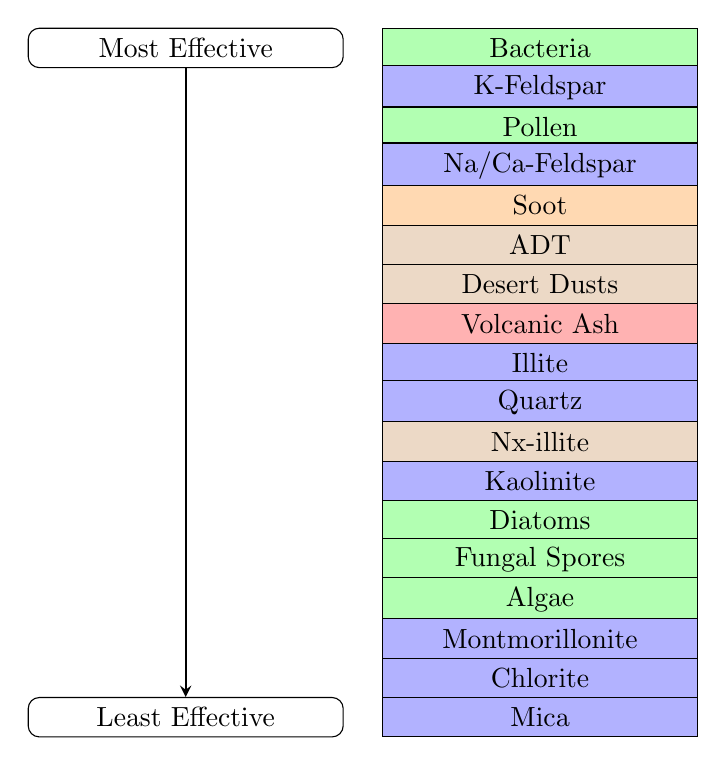
\begin{tikzpicture}[node distance=0.5cm]
	
	\node (scale) [label] {Most Effective};
	\node (1) [bio, right of=scale, xshift=4cm] {Bacteria};
	\node (2)	[mineral, below of=1] {K-Feldspar};
	\node (3)	[bio, below of=2] {Pollen};
	\node (4)	[mineral, below of=3] {Na/Ca-Feldspar};
	\node (4b) [carbonaceous, below of=4] {Soot};
	\node (5)	[dust, below of=4b] {ADT};
	\node (6)	[dust, below of=5] {Desert Dusts};
	\node (7)	[ash, below of=6] {Volcanic Ash};
	\node (8)	[mineral, below of=7] {Illite};
	\node (9)	[mineral, below of=8] {Quartz};
	\node (10)	[dust, below of=9] {Nx-illite};
	\node (11)	[mineral, below of=10] {Kaolinite};
	\node (12)	[bio, below of=11] {Diatoms};
	\node (13)	[bio, below of=12] {Fungal Spores};
	\node (14)	[bio, below of=13] {Algae};
	\node (15)	[mineral, below of=14] {Montmorillonite};
	\node (16)	[mineral, below of=15] {Chlorite};
	\node (17)	[mineral, below of=16] {Calcite};
	\node (17)	[mineral, below of=16] {Mica};
	\node (scale2) [label, left of=17, xshift=-4cm] {Least Effective};
	\draw [arrow] (scale) -- (scale2);
	
	\end{tikzpicture}
	\caption{Approximate order of various ice nucleating particles from most effective to least effective. Green indicates bioaerosols. Blue indicates pure minerals. Orange indicates carbonaceous combustion aerosols. Brown indicates dusts (both natural and artificial). Red indicates volcanic ash. Order based on results from \cite{dieh2002}, \cite{knop2011}, \cite{mur2012}, \cite{pumm2012}, \cite{atk2013}, \cite{aug2014}, \cite{emer2015}, \cite{whal2015}, and \cite{zol2015}}
	\label{fig:INP}
\end{figure}

\subsubsection{Mineral Dusts}
Mineral dusts are some of the most common INPs \citep{mur2012}. The emission of global dust aerosols is estimated to be between \SI{1000}{Tg} and \SI{3000}{Tg} per year \citep{thor2011}. Most of the dust is assumed to originate from the ``global dust belt'' that extends from North Africa eastward to China \citep{pros2002}. Although some of the largest and most well studied dust sources are arid tropical to mid-latitude regions, dust emission is a global phenomenon \citep{bull2016}.

Dust is a broad term to cover a range of mixtures and pure mineral powders. The mineral composition of dust is key to the ability of a dust to act as an INP because ice nucleation occurs at discrete nucleation sites on the particles and the effectiveness of those nucleation sites depends on the physiochemical characteristics of the sites.

The bulk composition of atmospheric dust is almost 50\% clays, primarily illite followed by kaolinite, chlorite, and montmorillonite. Quartz is the next most common mineral in atmospheric dust at around 30\%, followed by feldspars at around 13\%, and then other minerals making up the rest. \citep{mur2012} The composition of dust aerosols in a specific location depends on the geology of the source region and how far the aerosols have traveled from the source. Dust aerosols collected near the source can have a substantially different composition than the same dust collected far from the source because of weathering and sedimentation during transport \citep{mur2012}.

\subsubsection{Bioaerosols}
Bioaerosols are aerosol particles that originate from living organisms. Bioaerosols include: bacteria, lichen and fungi, diatoms and algae, and pollen \citep{mur2012,fro2016}. It is estimated that bioaerosols may make up around 20\% of the total aerosol amounts \citep{jaen2005,jaen2007}. The typical size of bioaerosols ranges from around \SI{1}{\mu m} to \SI{100}{\mu m} and they can have residence times in the atmosphere of several days \citep{bur2009, mur2012,fro2016}.

Bioaerosols are some of the most effective INP that have been studied. Bacteria in particular have been shown to be highly effective INP and are the only aerosol observed to trigger nucleation above \SI{-10}{\degreeCelsius}. Other forms of bioaerosols have been less heavily studied than bacteria but have been seen to be active INP in the freezing temperature range between those of bacteria and mineral powders. \citep{dieh2002, knop2011, mur2012, pumm2012}

\subsubsection{Carbonaceous Combustion Aerosols}
Another type of aerosol that can potentially act as INP is carbonaceous combustion aerosols. These aerosols are produced during combustion and include soot, black carbon, and brown carbon. The definitions of soot, black carbon, and brown carbon are not rigorously defined and are sometimes used interchangeably but in general black carbon is composed almost exclusively of elemental carbon, brown carbon is composed of little to no elemental carbon, and soot is a general term for any particles formed from incomplete combustion \citep{lon2013}. The composition of carbonaceous combustion aerosols varies widely from pure elemental carbon to combinations of organic and inorganic materials depending on the conditions and fuel used in the combustion. \citep{spra2011,mur2012,ull2017}

There is clear evidence of carbonaceous combustion aerosols acting as CCN, with one study estimating that they make up more than half of the global CCN concentration and an even greater percentage in highly polluted areas \citep{spra2011}. The ability to act as INP in the atmosphere is less clear because field observations have given conflicting results \citep{mur2012}. However, laboratory studies have confirmed that carbonaceous combustion aerosols can nucleate ice and that the nucleation temperature and ice-active surface site density values depend on the origin of the particles \citep[e.g.][]{demo1990, dieh1998, pett2009}. Data from two studies on ice nucleation by soot showed ice-active surface site density values slightly higher than dust and pure minerals over the same temperature range \citep{mur2012}.

\subsubsection{Volcanic Ash}
Volcanic ash is another potential source of INP, though the impact is episodic and limited to times around volcanic events. The impacts of volcanic events can be far reaching as they have been known to cause increases of INP amounts in locations over \SI{4000}{km} away from the source \citep{bing2012}. The size, shape, and composition of volcanic ash depends on the source region, the type of eruption, and the viscosity of the magma \citep{heik1972}. The composition of volcanic ash includes a mixture of minerals and volcanic glass. The minerals in volcanic ash can be similar to those found in mineral dusts. Some common minerals found in volcanic ash include: quartz, feldspar, mica, olivines, pyroxenes, and amphiboles \citep{horw2006, dura2010, dags2013}. The size of volcanic ash particles ranges from \SI{0.1}{\mu m} to \SI{2000}{\mu m} \citep{dura2010}. The volcanic ashes studied by \cite{forn2009}, \cite{hoyl2011}, and \cite{stei2011} showed ice-active surface site density values on par or slightly higher than the mineral dusts from other studies \citep[e.g.][]{mur2012,ull2017}.

\subsubsection{Contribution of INP Types}
Evaluating the contribution of the different types of INP is challenging because the contributions vary depending on location and time. Generally speaking, mineral dusts are among the most common aerosols in the atmosphere and bioaerosols are active at the highest temperatures \citep{mur2012}. Volcanic ash is limited to times around volcanic events and plant-based bioaerosols depend greatly on location and season. There is also always the chance that there could be an as of yet unidentified INP source.

%\chapter{Cloud Droplet Formation} \label{ch:act}
\section{Cloud Droplet Formation} \label{ch:act}
Liquid drops form from the condensation of water vapour through either homogeneous or heterogeneous nucleation \citep{rog1989,lamb2011}. In homogeneous nucleation, liquid drops are formed due to the random collisions of water vapour molecules. When water molecules collide, there is a chance that they will stick together and form a cluster. Such clusters are relatively unstable until they reach a large enough size for the rate of condensation to exceed the rate of evaporation. The supersaturation values required to get clusters to a large enough size are higher than are generally observed in the atmosphere, so, while homogeneous nucleation of liquid drops is theoretically possible, it is generally considered insignificant for cloud processes. \citep{mcdo1958, rog1989, lamb2011}

Heterogeneous nucleation involves water condensing on an aerosol particle (CCN) and is generally the only way clouds can form in the atmosphere. Aerosols can be classified as either soluble (i.e. dissolves in water) or insoluble (i.e. does not dissolve in water) and each type impacts nucleation in slightly different ways. When water condenses onto an insoluble particle a spherical cap of liquid forms on the surface of the particle. The dimensions of the cap depend on the hygroscopicity of the particle. The cap will be nearly flat on hydrophilic surfaces and domed on hydrophobic surfaces \citep{lamb2011}. Figure \ref{fig:flatNuc} shows the relationships between hygroscopicity and contact angle and contact angle and supersaturation needed to nucleate a liquid drop on a solid flat surface. For spherical aerosol particles, the required supersaturation also depends on the size of the particle, with larger particles requiring lower supersaturations than smaller particles of the same hygroscopicity (see Figure \ref{fig:sphereNuc}).

Insoluble aerosols lower the supersaturation needed for drop formation by reducing the curvature of the forming drop. This is due to the curvature effect which describes how the probability of evaporation increases with curvature (i.e. greater curvature means it is easier for molecules to escape the drop). \citep{rog1989, lamb2011,bouc2015}

\begin{figure}[H]
	\centering
	\includegraphics[scale=0.4]{/home/vtrost/Documents/PhD/PhD_writing/Thesis/Figures/flatNuc.png}
	\caption{Diagram comparing the contact angle of a liquid water drop on a flat surface to the saturation ratio required to initiate nucleation. The x-axis is contact angle in degrees and represents how hydrophilic or hydrophobic the surface is. Hydrophobic surfaces have large contact and hydrophilic surfaces have small contact angles. The y-axis is the threshold saturation ratio which represents the amount of saturation or supersaturation required to initiate nucleation. The minimum of the plot (i.e. a saturation ratio of 1) represents saturation and the maximum of the plot represents a supersaturation value high enough for homogeneous nucleation to occur. This diagram highlights how the more hydrophilic a surface is the lower the required supersaturation for nucleation is. \citep[][Figure 7.9]{lamb2011}}
	\label{fig:flatNuc}
\end{figure}

\begin{figure}[H]
	\centering
	\includegraphics[scale=0.4]{/home/vtrost/Documents/PhD/PhD_writing/Thesis/Figures/sphereNuc.png}
	\caption{Diagram illustrating the relationship between particle radius, contact angle of a liquid droplet on the particle, and the saturation ratio required for nucleation to occur. The x-axis is particle radius in \SI{}{\mu m} and the y-axis is threshold saturation ratio for nucleation. The three lines correspond to three different contact angles (\ang{90}, \ang{60}, \ang{0})  between the particle and a liquid droplet on the surface of the particle. Higher contact angles correspond to particles of higher hydrophobicity. The diagram shows that the supersaturation required for nucleation decreases with decreasing contact angle and increasing particle radius. \citep[][Figure 7.10]{lamb2011}}
	\label{fig:sphereNuc}
\end{figure}

Soluble aerosols are more effective CCN than insoluble aerosols because soluble particles can take advantage of both curvature and solute effects. The solute effect describes how condensation is enhanced by dissolved solute ions decreasing the equilibrium vapour pressure of the solution and thereby reducing the rate of evaporation and increasing the rate of condensation. The solute effect tends to dominate the curvature effect which is why soluble particles are generally more effective CCN than insoluble particles. As water molecules collect on the surface of a soluble particle they bond with the ions in the particle and begin to break down the bonds between the particle molecules leading to deliquescence of the particle and the formation of a liquid solution drop. \citep{rog1989,lamb2011,bouc2015}

In addition to being classified based on solubility, CCN can also be classified as either unactivated or activated based on the size of the liquid drop they are part of. An activated aerosol is one which is part of a drop that is larger than the peak in the K\"ohler curve for the specific aerosol \citep{rog1989,bouc2015}. Figure \ref{fig:kohler} is an example of a K\"ohler curve for an ammonium sulfate aerosol. Drops that have a radius smaller than $r^{*}$, which is known as the critical radius and is the radius value associated with the peak of the K\"ohler curve, are known as haze particles. Haze particles are in stable equilibrium with the surrounding environment. In other words, as the saturation of the environment changes the haze particle will grow or shrink until it is again at equilibrium. Cloud particles (i.e. drops with radius larger than $r^{*}$), however, are unstable because their equilibrium saturation value is below that of the environment and so water vapour will be able to condense and the drop grow as long as the environment saturation value stays above the equilibrium curve. \citep{rog1989, lamb2011}

\begin{figure}[H]
	\centering
	\includegraphics[scale=0.45]{/home/vtrost/Documents/PhD/PhD_writing/Thesis/Figures/kohler.png}
	\caption{K\"ohler curve for an ammonium sulfate aerosol. The x-axis is a log-scale of drop radius in \SI{}{\mu m} and the y-axis is saturation ratio. The solid line is the K\"ohler curve, the top dashed line is the curvature term, and the bottom dashed line is the solution term. The peak of the K\"ohler curve, (S*, r*) represents the point at which a liquid drop will continue to grow in unstable equilibrium as long as the ambient saturation ratio remains above the K\"ohler curve. \citep[][Figure 6.2]{rog1989}}
	\label{fig:kohler}
\end{figure}

\subsection{Activation Parameterizations}
There are a range of methods used to calculate the number of activated aerosols in numerical models. Most activation parameterizations focus on calculating the maximum supersaturation because K\"ohler theory can accurately give the number of activated aerosols if the maximum supersaturation is known. Calculations can be performed either iteratively or non-iteratively, with iterative methods generally being significantly more computationally expensive than non-iterative ones. Most parameterizations include several reasonable assumptions \citep{Ghan2011}:
\begin{enumerate}
	\item{No cloud drops are present before cooling starts}
	\item{Cooling is adiabatic}
	\item{The aerosol population is represented by a size distribution with a uniform bulk hygroscopicity}
	\item{Aerosol particle composition is internally mixed}
	\item{The volume of particle water at maximum supersaturation is significantly greater than the dry aerosol volume}
	\item{The number of nucleated drops is determined by the number of aerosol particles with a critical supersaturation value that is less than the ambient maximum supersaturation}
	\item{Particles grow in equilibrium with relative humidity while the ambient supersaturation is less than the particle critical supersaturation}
	\item{After activation, growth rate is not significantly impacted by the curvature and solute effects}
\end{enumerate}

These assumptions are all well characterized in the current understanding of typical atmospheric conditions and activation physics.

Activation parameterizations in models can be as simple as activating a fixed number or can be represented by complex calculations involving details about the chemical properties of the aerosols. The following sections give examples of activation parameterizations that can be used in numerical models. All the parameterizations listed here are included in the Cloud AeroSol Interactions Microphysics (CASIM) scheme. (See \cite{casimCode}: activation.F90 and aerosol\_routines.F90 for details)

\subsubsection{Fixed Number (CASIM options default and 1)}
The simplest method is to activate a fixed number of aerosols. This could either be a constant value which does not depend on any other variables or it could be a fraction of the number of aerosol particles available. In CASIM the options are either a fixed cloud number equal to 50.0e6 or 100\% of the available aerosols.

\subsubsection{Twomey law (CASIM option 2)}
\cite{twom1959} derived an expression for the number of activated aerosols as a function of vertical wind speed. This expression, often known as the Twomey law, assumes that drops grow from an initial radius of zero when the ambient supersaturation reaches a critical value. The Twomey law is represented by Eq. \ref{eq:twom}

\begin{equation} \label{eq:twom}
N(w) = 0.88 \left(C^{\frac{2.0}{(K+2.0)}}\right) \left(7.0e^{-2}(100.0w)^{1.5}\right)^{\left(\frac{K}{K+2.0}\right)}
\end{equation}  

where \textit{N} is the number of activated aerosols (in \SI{}{cm^{-3}}), \textit{w} is the vertical wind (in \SI{}{m/s}), and \textit{C} and \textit{K} are airmass parameters (in CASIM these are set to 100.0 and 0.4 respectively).

Details of the aerosol size distribution and aerosol physiochemical properties are not considered. The Twomey parameterization is one of the first parameterizations that was developed and is often used as the starting point for most subsequent parameterizations. \citep{twom1959, rog1989, arg1998, arg2000}

\subsubsection{Abdul-Razzak and Ghan (CASIM option 3 and 4)}
Based on the activation parameterizations of \cite{twom1959} and \cite{ghan1993}, \cite{arg1998} developed a parameterization that calculates the number concentration of activated particles in terms of vertical wind, aerosol number concentration, aerosol composition, mode radius, and aerosol size distribution standard deviation. \cite{arg2000} extended this parameterization further by adapting the single mode parameterization of \cite{arg1998} to be applicable to aerosol distributions with multiple modes. The Abdul-Razzak and Ghan parameterization is divided into fifteen equations (Eq \ref{eq:arg1}-\ref{eq:arg15}) which combine to result in the number concentration of activated aerosols. (Table \ref{tab:argVariables} lists all the variables in the equations along with their values and units.)

The first step is to calculate the curvature effect coefficient, \textit{A}, using Eq \ref{eq:arg1} 
\begin{equation} \label{eq:arg1}
A(T) = \frac{2.0 \tau M_w}{R_u T \rho_w}	
\end{equation}

The second step is to calculate $\alpha$, a size-invariant coefficient, using Eq \ref{eq:arg2}
\begin{equation} \label{eq:arg2}
\alpha(T) = \frac{g (\frac{L_v}{R_r c_p T} - 1)}{T R_d}
\end{equation}

The third step is to calculate the saturation vapour pressure, $e_s$, using Eq \ref{eq:arg3}
\begin{equation} \label{eq:arg3}
e_s(T_c) = (611.21) exp\left((\frac{18.678-T_c}{234.5})(\frac{T_c}{257.14 + T_c})\right)
\end{equation}

The fourth step is to calculate a second size-invariant coefficient, $\gamma$, using Eq \ref{eq:arg4}
\begin{equation} \label{eq:arg4}
\gamma(p,T) = \frac{R_r p}{e_s + L_v^{\frac{2}{R_V T^{2} c_p}}}
\end{equation}

The fifth step is to calculate the growth coefficient, \textit{G}, using Eq \ref{eq:arg5}
\begin{equation} \label{eq:arg5}
G(T) = \frac{1}{\rho_w \left(\frac{R_v T}{e_s D_v} + \frac{L_V(\frac{L_V}{(R_v T)-1})}{K_a T}\right)}
\end{equation}

The sixth step is to calculate the dimensionless term $\zeta$ using Eq \ref{eq:arg6}
\begin{equation} \label{eq:arg6}
\zeta(w) = \left(\frac{2.0}{3.0}\right) A_k \left(\frac{w \alpha}{G}\right)^{0.5}
\end{equation}

The first six equations are functions of ambient conditions (temperature, pressure, and wind). The next five equations are functions of the aerosol population. The seventh step is to calculate the solute effect coefficient, $B_k$, using Eq \ref{eq:arg7}
\begin{equation} \label{eq:arg7}
B_k(i,\rho_{aero},M_{aero}) = \frac{i M_w \rho_{aero}}{M_{aero} \rho_w}
\end{equation}

The eighth step is to calculate the critical supersaturation, $s_{cr}$, using Eq \ref{eq:arg8}
\begin{equation} \label{eq:arg8}
s_{cr}(r_d) = \left(\frac{2.0}{\sqrt{B_k}}\right) \left(\frac{A_k}{3.0 r_d}\right)^{1.5}
\end{equation}

The ninth step is to calculate the dimensionless term, $\eta$, using Eq \ref{eq:arg9}
\begin{equation} \label{eq:arg9}
\eta(w,N) = \frac{(\frac{w \alpha}{G})^{1.5}}{2.0 \pi \rho_w \gamma N}
\end{equation}

The tenth and eleventh steps are to calculate $f_1$ (Eq \ref{eq:arg10}) and $f_2$ (Eq \ref{eq:arg11}), which are functions of the standard deviation of the aerosol size distribution and are used in Eq \ref{eq:arg12}
\begin{equation} \label{eq:arg10}
f_1(\sigma) = 0.5 exp(2.5(ln(\sigma))^{2})
\end{equation}

\begin{equation} \label{eq:arg11}
f_2(\sigma) = 1.0 + 0.25ln(\sigma)
\end{equation}

The next three equations are combinations of the previous equations. Steps twelve and thirteen are used together to calculate the maximum supersaturation using Eq \ref{eq:arg12} and Eq \ref{eq:arg13}. Note that \ref{eq:arg12} is a running sum over all the aerosol modes and \ref{eq:arg13} uses the final result of that running sum.
\begin{equation} \label{eq:arg12}
rsmax2_{(i+1)} = rsmax2_{(i)} + \frac{f_1(\frac{\zeta}{\eta})^{1.5} + f_2(\frac{s_{cr}^{2}}{\eta + 3.0\zeta})^{0.75}}{s_{cr}^{2}}
\end{equation}

\begin{equation} \label{eq:arg13}
smax = \sqrt{\frac{1.0}{rsmax2}}
\end{equation}

The fourteenth step is to calculate the error function based on the aerosol size distribution using Eq \ref{eq:arg14}
\begin{equation} \label{eq:arg14}
error\_func = 1.0 - erf\left(\frac{2ln(\frac{s_{cr}}{smax})}{3.0\sqrt{2.0}ln(\sigma)}\right)
\end{equation}

The final step is to calculate the number of activated aerosols using Eq \ref{eq:arg15}
\begin{equation} \label{eq:arg15}
nccn(N) = 0.5 N error\_func
\end{equation}

Within a model, the results from Eq \ref{eq:arg15} are constrained to keep them within reasonable limits. In CASIM this means ensuring that \textit{nccn} is never greater than the number of available aerosols nor smaller than a minimum threshold (specifically $0.1e6$ \SI{}{m^{-3}}). The equations above are evaluated for each aerosol type and mode used in the model.

\begin{table}[h]
	\centering
	\caption{List of variables used in the Abdul-Razzak \& Ghan activation parametrization. The first column is the variable symbol used in the equations. The second column is the name or description of what the variable represents. The third column is the value of the variable. Values are either commonly accepted constant values or the values used in CASIM for variables that have multiple possible values.}
	\label{tab:argVariables}
	\begin{tabular}{|l|l|l|}
		\hline
		\textbf{Symbol} & \textbf{Name}                                      & \textbf{Value and Units} \\ \hline
		$c_p$           & heat capacity of air                               & \SI{1005}{J/kg K}        \\ \hline		
		$D_v$           & diffusivity of water vapour in air                 & 0.226e-4 \SI{}{m^{2}/s}   \\ \hline
		g               & gravitational acceleration                         & \SI{9.81}{m/s^{2}}       \\ \hline
		i               & van't Hoff factor of the aerosol                   &                          \\ \hline
		$k_a$           & thermal conductivity of air                        & 0.243e-1 \SI{}{W/m K}     \\ \hline
		$L_v$           & latent heat of vaporization                        & 0.2501e7 \SI{}{J/kg}      \\ \hline
		$M_{aero}$      & molecular weight of aerosol particle               & \SI{}{kg/mol}            \\ \hline
		$M_w$           & molecular weight of water                          & 0.18015e-1 \SI{}{kg/mol}  \\ \hline
		N               & aerosol number concentration                       & \SI{}{m^{-3}}            \\ \hline
		p               & pressure                                           & Pa                       \\ \hline
		$r_d$           & radius of aerosol particle                         & \SI{}{m}                 \\ \hline
		$R_d$           & gas constant of dry air                            & \SI{287.05}{J/kg K}      \\ \hline
		$R_r$           & ratio of gas constants of water vapour and dry air & \SI{1.6077}{}            \\ \hline
		$R_u$           & universal gas constant                             & \SI{8.314472}{J/K mol}   \\ \hline
		$R_v$           & gas constant of water vapour                       & \SI{461}{J/kg K}         \\ \hline
		$\rho_{aero}$   & density of aerosol particle                        & \SI{}{kg/m^{3}}          \\ \hline
		$\rho_w$        & density of water                                   & \SI{997}{kg/m^{3}}       \\ \hline
		$\sigma$        & standard deviation of aerosol size distribution    & \SI{}{m}                 \\ \hline			
		T               & temperature                                        & K                        \\ \hline
		$\tau$          & surface tension                                    & 0.8e-1 \SI{}{J/m^{2}}     \\ \hline
		$T_c$           & temperature                                        & \SI{}{\degreeCelsius}    \\ \hline
		w               & vertical wind                                      & \SI{}{m/s}               \\ \hline
		rsmax2			& square of maximum supersaturation					 & 							\\ \hline
		smax			& maximum supersaturation							 &							\\ \hline
		$error_{func}$	& error function									 &							\\ \hline
		nccn			& number of activated aerosols						 & \SI{}{m^{-3}}			\\ \hline
	\end{tabular}
\end{table}

\subsubsection{Shipway 2015 (CASIM option iopt\_shipway\_act)}
Another way to reduce the activation calculations to something that is computationally feasible is to reduce the number of independent variables to allow the integrals to be pre-calculated and evaluated using lookup tables. \cite{ship2015} provides a derivation of such a parameterization (see that paper for details).

\section{Ice Nucleation} \label{ch:iceNuc}
Ice nucleation refers to the initial appearance of the solid phase \citep{vali2015}. Nucleation occurs when molecules bond in specific structures. In the case of water, eighteen ice structures have been identified \citep{bai2012}, though most of those form under extremely low temperatures or high pressures. Under normal atmospheric conditions, two structures are possible. The most common form is hexagonal but cubic is also possible in the stratosphere and the top of the troposphere \citep{hobbs1974,murp2003}. Hexagonal ice will be the assumed atomic crystal structure in this thesis. Hexagonal ice is a centrosymmetric solid with hexagonal symmetry. Its structure is defined by hexagonal rings of water molecules with an oxygen atom at each vertex. \citep{hobbs1974} Figure \ref{fig:waterStructure} shows a diagram of the molecular structure of the three phases of water.

At the fundamental level, ice is formed simply through the collisions and bonding of water molecules as decreasing temperature results in decreased molecule speeds and increased bonding potential \citep{chal1959}. In the atmosphere, however, there is more to consider than just temperature. In fact, depending on the environment, ice nucleation can occur at any temperature between \SI{0}{\degreeCelsius} and \SI{-40}{\degreeCelsius} \citep{rog1989}. There are five ice nucleation processes that have been identified to explain how ice nucleation occurs depending on temperature and the interactions between water vapour, liquid water, ice, and aerosols. Those five nucleation processes are described in detail below.

\begin{figure}[H]
	\centering
	\includegraphics[width=\textwidth]{/home/vtrost/Documents/PhD/PhD_writing/Thesis/Figures/waterStructure.jpg}
	\caption{Diagram of the molecular structure of the three phases of water. Oxygen atoms are represented by the large, blue circles, hydrogen atoms by the small, green circles, and hydrogen bonds between water molecules by the dashed lines. The left diagram represents the physical state (in the form of hexagonal ice), the middle diagram is the liquid state, and the right is the gas state. \citep{waterStructure}}
	\label{fig:waterStructure}
\end{figure}

\subsection{Ice Nucleation Processes}
The five ice nucleation processes can be divided into two types: homogeneous processes and heterogeneous processes. Homogeneous processes involve pure water free from other substances. Heterogeneous processes require particles of a different substance to be mixed in with the water, either dissolved within the liquid water or as insoluble particles.

\subsubsection{Homogeneous Freezing}
Homogeneous freezing is the simplest of the processes because it involves only the fundamental concept of freezing without any additional mechanisms involved. Homogeneous nucleation occurs when the water molecules in a pure water drop bond into the ice structure. The random motions and relatively weak hydrogen bonds mean that pure water can remain in an unfrozen, supercooled state down to around \SI{-40}{\degreeCelsius} after which any further cooling will result in spontaneous, homogeneous freezing \citep{rog1989}. Homogeneous deposition, which is the process of pure ice forming directly from water vapour without any additional substances, is theoretically possible as well but is not considered a cloud ice nucleation process because it requires supersaturations that exceed those observed in the atmosphere \citep{vali2015}.

\subsubsection{Heterogeneous Nucleation}
When water is mixed with impurities, either as substances dissolved in liquid water or as insoluble aerosol particles, ice nucleation occurs through one of four heterogeneous nucleation processes \citep{rog1989,lamb2011,kanj2017}. Figure \ref{fig:iceNuc} shows a diagram of the four processes. The first process is deposition nucleation. In deposition nucleation, ice forms directly on an aerosol from the water vapour phase. Next is condensation freezing which involves water vapour condensing onto an aerosol particle and then the resulting liquid drop freezing. In contact freezing, a pre-existing liquid drop collides with an aerosol particle and freezing is triggered at the point of contact. The last process is immersion freezing, which is considered to be the most dominant process in mixed-phase clouds \citep{aug2014,tobo2016}. In immersion freezing, freezing is triggered by an aerosol particle that is immersed in a liquid drop.

\begin{figure}[h]
	\centering
	\includegraphics[scale=0.7]{/home/vtrost/Documents/PhD/PhD_writing/Thesis/Figures/iceNuc.png}
	\caption{Diagram of the four heterogeneous ice nucleation mechanisms (from top to bottom: deposition, condensation freezing, contact, and immersion). The small squares represent an aerosol particle, the circles represent a liquid drop, the hexagons represent an ice crystal, and the arrows represent the evolution through the different stages of nucleation. \citep[][Figure 9.1]{rog1989}}
	\label{fig:iceNuc}
\end{figure}

\subsection{Ice Nucleation Parameterizations}
Due to the small scale and high complexity of ice nucleation processes, it is often not possible to fully resolve ice nucleation in numerical models, excluding small scale models designed specifically to isolate and simulate cloud processes. Instead, parameterizations, which use a set of assumptions and estimations to calculate approximations for ice nucleation under certain conditions and for specific nucleation processes, must be used. In this way it is possible to simulate ice nucleation within larger scale models without overloading the computer system or causing impractical run times. 

There have been many ice nucleation parameterizations developed over the last 60+ years and the development of new and improved parameterizations is an area of continual research. The following sections give an overview of some of the most commonly used ice nucleation parameterizations (which are also the parameterizations available in CASIM). All these parameterizations calculate ice nucleation in terms of either immersion freezing, contact freezing, or both. Other ice nucleation methods are not considered. In the equations below, $dN_{contact}$ is the number concentration of ice particles formed through contact freezing and $dN_{imm}$ is the number concentration of ice crystals formed through immersion freezing. (All ice nucleation parameterizations are found in \cite{casimCode}: ice\_nucleation.F90.)

\subsubsection{Basic Contact Nucleation (CASIM option 5)}
The simplest method is to nucleate a set fraction of the INP population or to calculate nucleation based only on the INP number concentration and one other independent variable that does not depend on environmental characteristics. For example, in Eq \ref{eq:case5} contact nucleation is calculated as the difference between the number of INPs and the number of pre-existing ice crystals.

\begin{equation} \label{eq:case5}
dN_{contact} = N - ice\_number
\end{equation}

where total $N$ is the INP number concentration and $ice\_number$ is the number concentration of pre-existing ice crystals.


\subsubsection{Fletcher 1962 (CASIM option 3)}
One of the earliest ice nucleation parameterizations was derived by \cite{flet1962}. The parameterization, given by Eq \ref{eq:flet}, is a relatively simple one because it depends only on temperature (and air density to convert the number to number concentration).

\begin{equation} \label{eq:flet}
dN_{imm} = \frac{0.01\exp(-0.6T_c)}{\rho}
\end{equation}

where $T_c$ is temperature (in \SI{}{\degreeCelsius}) and $\rho$ is air density.


\subsubsection{Cooper 1986 (CASIM option default)}
\cite{coop1986} developed a parameterization in the same form as the Fletcher parameterization but using different constants. The parameterization is given by Eq \ref{eq:coop}

\begin{equation} \label{eq:coop}
dN_{imm} = \frac{5.0\exp(0.304T_c)}{\rho}
\end{equation}

where $T_c$ is temperature (in \SI{}{\degreeCelsius}) and $\rho$ is air density.


\subsubsection{Meyers 1992 (CASIM option 2)}
\cite{meye1992} derived a slightly more complex parameterization compared to Fletcher and Cooper but like those the Meyers parameterization only depends on temperature and does not consider the ambient aerosol population. The parameterization was derived by fitting a line to the results from two continuous-flow chamber experiments and is considered valid for environments between temperatures of \SI{-7}{\degreeCelsius} to \SI{-20}{\degreeCelsius}, ice supersaturation between $2\%$ to $25\%$, and liquid supersaturation between $-5\%$ to $4.5\%$ \citep{meye1992}. The parameterization is divided into three equations (Eq \ref{eq:mey1} - Eq \ref{eq:mey3}) with the first two equations being terms within the third equation as follows

\begin{equation} \label{eq:mey1}
lws = 6.112\exp\left(\frac{17.62T_c}{243.12 + T_c}\right)
\end{equation}

\begin{equation} \label{eq:mey2}
is = 6.112\exp\left(\frac{22.46T_c}{272.62 + T_c}\right)
\end{equation}

\begin{equation} \label{eq:mey3}
dN_{imm} = \frac{1.0e^{3}\exp(A_m+B_m(100.0(\frac{lws}{is}-1.0)))}{\rho}
\end{equation}

where $lws$ is liquid water saturation vapour pressure, $is$ is ice saturation vapour pressure, $T_c$ is temperature (in \SI{}{\degreeCelsius}), $\rho$ is air density, and $A_m$ and $B_m$ are constants equal to -0.639 and 0.1296 respectively. 


\subsubsection{DeMott 2010 (CASIM option 4)}
Unlike the parameterizations above, the \cite{demo2010} parameterization calculates both immersion and contact freezing as functions of temperature and aerosol number concentration. The parameterization was derived by fitting a line to INP measurements from nine field studies of mixed-phase clouds at temperatures between \SI{-9}{\degreeCelsius} to \SI{-35}{\degreeCelsius}. The data excludes sea-salt aerosols, ignores differences in aerosol composition, and assumes that all aerosols have a diameter greater than \SI{0.5}{\mu m} \citep{demo2010}. Contact freezing is calculated using Eq \ref{eq:dm10_1} and immersion freezing is calculated using Eq \ref{eq:dm10_2}

\begin{equation} \label{eq:dm10_1}
dN_{contact} = \frac{1.0e^{3}}{\rho}A_{d10}(0.01-T_c)^{B_{d10}}(\rho (1.0e^{-6}) (0.0001) N)^{(C_{d10}(0.01-T_c)+D_{d10})}
\end{equation}

\begin{equation} \label{eq:dm10_2}
dN_{imm} = \frac{1.0e^{3}}{\rho}A_{d10}(0.01-T_c)^{B_{d10}}(\rho 1.0e^{-6} N_{act})^{(C_{d10}(0.01-T_c) + D_{d10})}
\end{equation}

where $T_c$ is temperature (in \SI{}{\degreeCelsius}), $N$ is the INP number concentration, $N_{act}$ is the number concentration of activated aerosols, $\rho$ is air density, and the four parameterization constants are $A_{d10} = 5.94e{-5}$, $B_{d10} = 3.33$, $C_{d10} = 0.0264$, and $D_{d10} = 0.0033$ (the \textit{d10} subscript indicates that the constant is associated with the Demott 2010 parameterization.).


\subsubsection{DeMott2010 version 2 (CASIM option 10)}
This parameterization is the same as the previous one except that insoluble and activated aerosols are treated together instead of separately. In the above parameterization, contact freezing was calculated by considering only insoluble aerosols and immersion freezing by considering only activated aerosols. In this parameterization, immersion freezing is calculated by considering both activated and insoluble aerosols (Eq \ref{eq:d10_2_1}), then contact freezing is calculated as the difference between the result of the immersion freezing calculation and the number of activated aerosols (Eq \ref{eq:d10_2_2}), and then the final number concentration of ice formed through immersion freezing is calculated by subtracting the result of Eq \ref{eq:d10_2_2} from Eq \ref{eq:d10_2_1}.

\begin{equation} \label{eq:d10_2_1}
dN_{imm} = \frac{1.0e^{3}}{\rho}A_{d10}(0.001 - T_c)^{B_{d10}}(1.0e^{-6}\rho(N_{act}+N))^{(C_{d10}(0.01-T_c)+D_{d10})}
\end{equation}

\begin{equation} \label{eq:d10_2_2}
dN_{contact} = dN_{imm} - N_{act}
\end{equation}

\begin{equation} \label{eq:d10_2_3}
dN_{imm} = dN_{imm} - dN_{contact}
\end{equation}

where $T_c$ is temperature (in \SI{}{\degreeCelsius}), $N$ is INP number concentration, $N_{act}$ is the number concentration of activated aerosols, $\rho$ is air density, and the four parameterization constants are $A_{d10} = 5.94e{-5}$, $B_{d10} = 3.33$, $C_{d10} = 0.0264$, and $D_{d10} = 0.0033$ (the \textit{d10} subscript indicates that the constant is associated with the Demott 2010 parameterization.).


\subsubsection{Niemand 2012 (CASIM option 7)}
\cite{niem2012} used data from cloud chamber studies of immersion freezing on desert dust to derive a parameterization for immersion freezing based on particle surface area and ice-active surface site density. Eq \ref{eq:nie1} is used to calculate the aerosol surface area in a volume of air. Eq \ref{eq:nie2} is used to calculate the ice-active surface site density as a function of temperature. Eq \ref{eq:nie3} combines the results from the previous equations to calculate the number concentration of new ice crystals.

\begin{equation} \label{eq:nie1}
S_A = 4\pi N_{act}\rho r_d^{2} \exp(2\sigma^{2})
\end{equation}

\begin{equation} \label{eq:nie2}
n_{sites} = \exp(-0.517T_c + 8.934)
\end{equation}

\begin{equation} \label{eq:nie3}
dN_{imm} = \frac{n_{sites} S_A}{\rho}
\end{equation}

where $N_{act}$ is the number concentration of activated aerosols, $\rho$ is air density, $r_d$ is the mean radius of the aerosols, $\sigma$ is the standard deviation of the aerosol size distribution, and $T_c$ is temperature (in \SI{}{\degreeCelsius}).


\subsubsection{Atkinson 2013 (CASIM option 8)}
The \cite{atk2013} parameterization is nearly the same as the \cite{niem2012} parameterization, the only difference is that the Atkinson parameterization is formulated specifically for K-feldspar. Eq \ref{eq:atk1} is the same as Niemand Eq \ref{eq:nie1} except for the addition of the factor of 0.35 to account for the assumed K-feldspar fraction in the dust population. Eq \ref{eq:atk2} takes on the same form as Niemand Eq \ref{eq:nie2} except the constants are determined by fitting a line to the K-feldspar immersion freezing studies as described in \cite{atk2013}.

\begin{equation} \label{eq:atk1}
S_A = (0.35)(4)\pi N_{act} \rho r_d^{2} \exp(2\sigma^{2})
\end{equation}

\begin{equation} \label{eq:atk2}
n_{sites} = \exp(-1.038T_k + 275.26)
\end{equation}

\begin{equation} \label{eq:atk3}
dN_{imm} = \frac{n_{sites}S_A}{\rho}
\end{equation}

where $N_{act}$ is the number concentration of activated aerosols, $\rho$ is air density, $r_d$ is the mean radius of the aerosols, $\sigma$ is the standard deviation of the aerosol size distribution, and $T_k$ is temperature (in \SI{}{K}).


\subsubsection{Tobo 2013 (CASIM option 9)}
The \cite{tobo2013} parameterization is based on the \cite{demo2010} parameterization but with fit parameters derived from a field experiment over a pine forest and is represented by Eq \ref{eq:tobo}

\begin{equation} \label{eq:tobo}
dN_{imm} = \frac{1.0e^{3}}{\rho}(\rho 1.0e^{-6} N_{act})^{A_t T_c + B_t} \exp(C_t T_c +D_t)
\end{equation}

where $\rho$ is air density, $N_{act}$ is the number concentration of activated aerosols, $T_c$ is temperature (in \SI{}{\degreeCelsius}), and the four parameterization constants are $A_t = -0.074$, $B_t = 3.8$, $C_t = 0.414$, and $D_t = -9.671$.


\subsubsection{DeMott 2015 (CASIM option 6)}
\cite{demo2015} derived a parameterization specifically for dust aerosols with diameter greater that \SI{0.5}{\mu m} based on a modify version of the \cite{tobo2013} parameterization. The parameterization is valid for temperatures between \SI{-21}{\degreeCelsius} to \SI{-35}{\degreeCelsius}.

\begin{equation} \label{eq:dm15_1}
dN_{contact} = \frac{1.0e^{3}}{\rho}c_f(\rho(1.0e^{-6})(0.0001)N)^{(A_{d15}T_c + B_{d15})}\exp(C_{d15}T_c + D_{d15})
\end{equation}

\begin{equation} \label{eq:dm15_2}
dN_{imm} = \frac{1.0e^{3}}{\rho}c_f (\rho N_{act} 1.0e^{-6})^{(A_{d15}T_c + B_{d15})}\exp(C_{d15}T_c + D_{d15})
\end{equation}

where $T_c$ is temperature (in \SI{}{\degreeCelsius}), $N$ is INP number concentration, $\rho$ is air density, and the five parameterization constants are $c_f = 1.0$, $A_{d15} = 0.0$, $B_{d15} = 1.25$, $C_{d15} = 0.46$, and $D_{d15} = -11.6$.

\section{Secondary Ice Production} \label{ch:sip}
Ice nucleation is not the only way to produce ice crystals in clouds. In fact, there are many cases where ice nucleation alone cannot account for the number of ice crystals observed in clouds \citep[e.g.][]{demo2010,oshea2017,sull2018}. At temperatures above the threshold for homogeneous nucleation, the number of ice crystals that can be produced through nucleation is limited by the number of INPs available to trigger heterogeneous nucleation. However, clouds are observed to contain orders of magnitude more ice crystals than would be expected based on the number of INPs available. This discrepancy is caused by secondary ice production processes multiplying the ice that is formed.

\subsection{Secondary Ice Production Processes}
Secondary ice production processes were being considered as early as the 1940s \citep{brew1949} and in the 1970s many detailed studies were performed to try to determine the exact processes at play \citep[e.g.][]{hal1974, moss1974, moss1978, vard1978}. Since then, four main secondary ice production processes have been defined: rime splintering, ice-ice collision fragmentation, drop shattering, and sublimation fragmentation.

\subsubsection{Rime Splintering (Hallett-Mossop)}
Riming is the ice crystal growth process in which an ice crystal grows due to supercooled droplets freezing on it upon collision \citep{lamb2011}. Under the right conditions the droplet can freeze in such a way that a spherical ice shell forms and then is ruptured from the internal pressure build-up. That rupturing causes ice splinters to be ejected and then those ice splinters can grow and continue to add to the ice formation process. \citep{field2017} This process of rime freezing and rupturing is known as rime splintering (also known as the Hallett-Mossop process, referred to simply as H-M for the rest of this thesis).

\cite{hal1974} and \cite{moss1974} performed laboratory experiments to determine the conditions required for H-M to occur. \cite{hal1974} found that H-M occurs within the temperature range of \SI{-8}{\degreeCelsius} to \SI{-3}{\degreeCelsius}, with peak production at \SI{-5}{\degreeCelsius}. The upper limit of \SI{-3}{\degreeCelsius} is because above that temperature accreted droplets tend to spread out before freezing instead of forming a spherical shell \citep{mack1967, choul1980, grig1983, dong1989, mason1996}.

\cite{moss1974} found that the rate of production depends on the number of drops with a diameter greater than \SI{23}{\mu m} that are available to be accreted. \cite{moss1978} did further studies and found that the presence of drops with a diameter less than \SI{13}{\mu m} is also required for secondary ice production. \cite{moss1985} refined the relationship even further by determining that H-M is most effective when larger drops are relatively rare compared to small drops. They were unable to define an optimum drop spectrum because it would vary with cloud temperature and rimer velocity, and so is not easily defined.

\cite{moss1985} also studied the impact of rimer velocity on splinter production. They found that if the relative velocity between the rimer and the drop is too high, then the drop tends to spread out over the ice surface thereby inhibiting splintering by not allowing an ice shell to form. If the relative velocity is too low, then the convective heat transfer in the accreted drop is too slow for an ice shell to form. For these reasons H-M is thought to occur within the rimer velocity range of \SI{0.2}{m/s} to \SI{5}{m/s}. Rimer velocity also impacts the high temperature cut-off and peak production temperature, with both decreasing as rimer velocity increases.

\subsubsection{Ice-ice Collision Fragmentation}
Another secondary ice production process is the fragmentation of ice crystals during ice-ice collisions. \cite{vard1978} used laboratory and mathematical model results to predict the amount of secondary ice particles produced via ice-ice collisions between different types of ice crystals. He determined that the most important factors were the relative velocity between ice crystals and the amount of riming on the crystals. Larger relative velocity leads to more forceful collisions and in turn a greater number of fragments ejected. Riming is also critical for collision fragmentation because it increases the fragility of the ice crystals. Even unrimed dendrites were found to be relatively ineffective at forming secondary ice production through collision fragmentation. The greatest secondary particle production was found to occur during collisions between graupel and rimed dendrites. 

Although rimed dendrites produce the most secondary particles during collisions, other types of ice particles can also produce significant amounts of secondary particles. \cite{taka1995} focused on graupel-graupel collisions. Through laboratory experiments they found peak secondary particle production at \SI{-16}{\degreeCelsius} during collisions between large and small graupel. They also suggest that the cause of the fragmentation ejection was the breaking of depositionally grown ice branches on the smaller graupel. Although ice-ice collisions can occur in any types of cloud where ice crystals are present, secondary ice production through collision fragmentation is most effective in convective clouds due to the turbulence increasing the collision frequency and updrafts allowing the growth of large graupel \citep{vard1978}.

\subsubsection{Drop Shattering}
Another secondary ice production process is the shattering of liquid drops as they freeze. This process is similar to rime splintering except that it is active in a stand-alone drop rather than a droplet that has been accreted onto an ice crystal. As the drop freezes from the outside in, the pressure within the growing ice shell increases until the shell shatters. During the freezing process, ice splinters can also be ejected as small ruptures and spicules form and break apart \citep{kei2020}. \cite{wild2017} recorded high speed videos of drops freezing and described in detail the freezing and ice ejection processes from initial nucleation to the final fragmentation of the drop.

Studies have shown that shattering is most probable for drops larger than \SI{50}{\mu m} in radius and for nucleation temperatures between \SI{-15}{\degreeCelsius} and \SI{-5}{\degreeCelsius} \citep[e.g.][]{mason1960, brow1968, frid2007}. \cite{phil2018} compiled data from six drop freezing lab studies and used that dataset to construct a numerical formulation for secondary ice production through drop shattering. They ran the formulation in a simplified parcel model and found that drop shattering could be a dominant secondary ice production method in some tropical convective cells.

\subsubsection{Sublimation Fragmentation}
Under certain conditions, sublimation fragmentation is also a source of secondary ice particles \citep{bacon1998}. As ice particles sublimate in undersaturated environments, thin branches or neck regions of the particles may decrease in diameter until the crystal fragments at that location. This means that sublimation fragmentation is most effective for branched crystal shapes such as dendrites and irregularly shaped crystals and aggregates. Sublimation fragmentation is only effective for ice multiplication if the undersaturated region of the cloud is small enough that the crystals reenter saturated regions before sublimating completely.

\subsubsection{Contributions of Secondary Ice Production Processes}
Evaluating the contribution of the various secondary ice production processes can be challenging and multiple processes can be active at the same time. It is generally assumed that for temperatures above \SI{-10}{\degreeCelsius} H-M is the dominant secondary ice production process because the other processes are most effective at lower temperatures \citep{oshea2017}. However, this is not necessarily always true. For example, \cite{yano2011} used a simplified model to compare ice multiplication through collision fragmentation and H-M. They show that the onset of H-M tends to be sooner than that of collision fragmentation because the latter requires the growth of larger graupel, so, where active, H-M would tend to dominate the ice multiplication. However, the multiplication from ice-ice collisions can be faster than that of H-M because H-M is linearly proportional to graupel number concentration and ice-ice collision fragmentation is proportional to the square of graupel number concentration. Changing conditions within the cloud or mixing from other environments can also cause the observed ice concentrations to be the result of multiple secondary ice production processes. The ability to evaluate the contributions of secondary ice production processes is further limited by the fact that models generally only simulated H-M if they simulate secondary ice production at all. This is starting to change, for example \cite{soti2021} developed a parameterization for ice-ice collision fragmentation, but the lack of parameterizations besides H-M is still a limitation to cloud ice modeling and the evaluation of secondary ice production processes in clouds.

\subsection{Sources of First Ice}
For any secondary ice production process to be active, an initial source of ice crystals is needed. The initial ice crystals can either be the results of ice nucleation or the input of pre-existing ice crystals from other sources.

\subsubsection{Ice Nucleation}
As discussed in Section \ref{ch:iceNuc}, there are five ice nucleation processes that could lead to ice formation in clouds. Limited INP amounts can mean that ice nucleation is unable to produce the amount of observed ice crystals but the few ice crystals that can be produced through nucleation can act as the source of first ice for secondary ice production processes.

\subsubsection{Blowing Snow}
One potential surface-based source of ice crystals is snow being lofted into the air, also known as blowing snow. Blowing snow generally occurs when wind speeds exceed \SI{7}{m/s} \citep{lach2010}, though characteristics such as topography, snow type and history, and temperature can change the minimum wind speed required (\cite{li1997, mah2003} and references therein). Blowing snow particles have been observed on days with wind speeds less than \SI{7}{m/s} which suggests that blowing snow can remain in the air for a couple days before settling back to the surface \citep{wald2003, lach2010}. The vertical extent of blowing snow can vary from a few meters to over \SI{100}{m} \citep{wald2003,palm2011}.

Blowing snow is composed of weathered and fractured ice crystals and aggregates, so the size of blowing snow particles can vary greatly. Measurements of blowing snow particle sizes range from approximately \SI{10}{\mu m} to \SI{450}{\mu m} depending on the date and location of the measurements \citep[e.g.][]{mah2003,nish2005,gord2009}. Larger particles tend to settle faster, so the particle size distribution shifts towards smaller sizes with increasing altitude. Blowing snow particles are often easy to distinguish from other types of ice crystals because they are typically smaller than falling snow and more spherical than cloud ice or diamond dust \citep{nish2005,lach2010}.

\subsubsection{Frost Flowers}
Frost flowers are another potential surface source of initial ice crystals. Frost flowers are dendritic ice crystals that form on the surface of young ice sheets and are most common in the autumn and winter \citep{domi2005, style2009}. The fragile structure of frost flowers suggests that they could easily fragment and become windblown, but the exact amount that is lofted is debatable \citep{rosc2011}.

\subsubsection{Hoar Frost and Sublimation Crystals}
Another potential surface source of initial ice crystals is hoar frost. Hoar frost is similar to frost flowers in that it is made up of depositionally grown ice crystals on a frozen surface but instead of forming on ice sheets it forms over snow. Hoar frost is generally associated with a downward flux of water vapour from the air to the snow surface. Crystals that form due to upward fluxes of water vapour from the snowpack are termed sublimation crystals. Depending on the environmental characteristics hoar frost and sublimation crystals can coexist and be challenging to differentiate between. Like frost flowers and blowing snow, under the right conditions hoar frost and sublimation crystals can become windblown and act as a surface-based source of ice crystals for secondary ice production. \citep{gal2014, far2016, feg2018}

\subsubsection{Advection and Seeding}
Ice crystals could also be advected in from other clouds or enter the cloud as precipitation from cloud layers above it (also known as cloud seeding). In these cases, ice is formed by ice nucleation in colder or more polluted environments where more INPs are active and then that ice moves into higher temperature or more pristine regions where it triggers ice multiplication by secondary ice production.

\subsubsection{Contributions of Initial Ice Sources}
The contribution of initial ice sources is not well defined and varies from case to case. Even for a set location the contributions would vary based on factors such as season, weather patterns, and aerosol loading.

\subsection{Outstanding Questions in Secondary Ice Production}
Despite years of research, there are still a number of outstanding questions about secondary ice production \citep{field2017,kei2020 ghbn  }. As mentioned previously, there are a number of possible secondary ice production processes that have been identified but which process is dominant in the atmosphere is still challenging to determine. Similarly, the prevalence of secondary ice production in the atmosphere and the types of clouds it is active in has not been well defined. Secondary ice production has been observed in many cloud types and locations but the dataset is still too small to make a definitive claim about the global distribution of secondary ice production. 

The exact details of the mechanisms involved are also not well understood. The general requirements of some secondary ice production processes are known but the physical mechanisms behind them are not fully understood. The role of INPs is also not well defined. It is known that some source of initial ice is required for secondary ice production to occur and that in many situations that will likely come from ice nucleation. What is not known is if there are specific ice nucleation processes or INPs that are most effective in triggering secondary ice production or what concentration of INPs are needed. 

Answers to these questions are needed to be able to properly simulate clouds in weather and climate models. Some ways to work towards answering these questions include: improved observations (of INPs, cloud characteristics, and secondary ice production processes), improved aerosol and ice parameterizations in models, and modeling studies comparing model outputs to observations and other models \citep{field2017}.

\chapter{Study of Antarctic Clouds}
\section{Antarctic Clouds and Climate} \label{ch:ant}
Recent field studies in Antarctica have shown cloud ice distribution patterns and amounts that cannot be explained by ice nucleation alone \citep[e.g.][]{oshea2017}. It is assumed that secondary ice production is acting to multiply a small number of initial ice crystals, but the exact secondary ice production process and initial ice sources involved are currently uncertain. With increasing amounts of in-situ cloud data from the region and improvements in instrumentation and numerical models it is becoming possible to quantitatively study the ice formation processes in Antarctic clouds. The following sections provide an overview of Antarctic weather, climate, and topography, as well as a discussion on the relevance of studying Antarctic clouds, the connection of such studies to climate and weather forecasting, and the key similarities and differences between the Antarctic and Arctic.

\subsection{Overview of Antarctic Weather and Climate}
Antarctica has some of the harshest weather on Earth \citep{laws2014}. The inland temperature ranges from \SI{-80}{\degreeCelsius} to \SI{-30}{\degreeCelsius} and along the coast the temperature ranges from \SI{-40}{\degreeCelsius} to \SI{10}{\degreeCelsius}. The continent is surrounded by the circumpolar trough and the interior is dominated by high pressure. Katabatic winds flow from the elevated interior down to the coast and can exceed \SI{100}{km/h} with gusts of over \SI{200}{km/h}. Due to the subsiding air and lack of moisture over the interior, the centre of the continent has relatively low amounts of cloud cover and precipitation, with both increasing to a maximum near the coast where there is more moisture available. \citep{antwx,lach2010,adhi2012,brom2012}

\begin{figure}[H]
	\centering
	\includegraphics[width=\textwidth]{/home/vtrost/Documents/PhD/PhD_writing/Thesis/Figures/antMap.png}
	\caption{Map of Antarctica including elevation contours, seas and ice sheets (labeled in blue), regions and mount ranges (labeled in black), and research bases (labeled in red). \citep{antMap}}
	\label{fig:antMap}
\end{figure}

\subsubsection{Topography}
Antarctica is divided into two asymmetric hemispheres divided by the Transantarctic Mountains. The East Antarctic ice sheet is larger and thicker than the West Antarctic ice sheet. The average elevation of the continent is \SI{2500}{m} above sea level but in the mountains and the central part of the East Antarctic ice sheet the elevation can exceed \SI{4000}{m} \citep{antTop}. Figure \ref{fig:antMap} shows a map of Antarctica, including the location of a few research bases (labelled in red).

\subsubsection{Cloud Cover}
The cloud cover over Antarctica varies both seasonally and geographically. \cite{town2007} performed an intercomparison of five cloud cover measurement techniques for the South Pole and determined that cloud cover ranged from a minimum of 45\% in the summer to a maximum of 65\% in the winter. \cite{brom2012} used satellite data to estimate the cloud cover over the ocean surrounding Antarctica and found it to range from 80\% to 95\% across all seasons. The cloud cover is highest over open ocean because sea ice tends to reduce cloud cover by around 10\% to 20\%, which leads to cloud cover along the coast of Antarctica being around 60\% to 80\%. In general, coastal cloud cover shows a winter minimum and summer maximum in response to the sea ice cycle but local topography can change that for individual locations. \citep{adhi2012}

\subsubsection{Cloud Microphysics}
Using an aircraft based lidar, \cite{morl1989} measured two cloud regimes present over western Antarctica. Over the lower-lying coast (in this case the Ross Ice Shelf) the clouds were observed to be mid-level liquid or mixed-phase clouds. Over the elevated South Pole plateau the clouds were higher ice clouds \citep{morl1989, lach2010}. \cite{oshea2017} measured stratus clouds over the Weddell Sea and coastal Antarctica and found the clouds to be mixed-phase clouds composed primarily of supercooled liquid water with variable patches of ice crystals. A range of ice crystal habits have been observed in Antarctic clouds including: plates, columns, rosettes, and Shimizu crystals \citep{laws2006, lach2010}.

\subsubsection{Aerosol Characteristics}
Antarctica's remote location and small population allow the Antarctic atmosphere to be relatively pristine and have lower aerosol concentrations than are measured in most other locations. Some of the aerosols found in Antarctica include: sea-salt, nitrates, and bioaerosols, such as methane sulphonic acid and sulfates \citep{rank2003,asmi2010,craw2017}. A year-long study of aerosols at the Halley research station, located on the Brunt Ice Shelf on the Weddell Sea, found that bioaerosols and nitrate aerosols were highest during the summer and sea salt was highest during the winter \citep{rank2003}.

Studies at Halley research station have determined that frost flowers are a dominant source of sea-salt aerosols for coastal Antarctica \citep[e.g.][]{rank2000, rank2003}. The impact of frost flowers on inland locations would depend on other factors such as the size of particles produced because larger particles tend to settle out before they can be transported far. The exact process of aerosol production from frost flowers is still uncertain. Mechanical weathering is one known process but it is thought that there could be other processes as well \citep{rank2003, xu2013}. A study by \cite{gior2018} using aerosol data collected near the Ross Ice Shelf suggests that blowing snow may also be an important source of aerosols in Antarctica.

There have been observations over the Southern Ocean of diatoms (a type of single cell algae \citep{saba2009}) being emitted into the atmosphere during bubble-bursting and wave-breaking. Another potential source of bioaerosols in Antarctica is penguin guano, although the exact emission rates are still uncertain. Fungal spores and pollen have been measured in Antarctica and airmass trajectory analysis suggests that those particles arrived at Antarctica via long-range transport from South America. \citep{craw2017} In 2015, \cite{craw2017} collected observations of airborne bio-fluorescent aerosols Halley research station and found that there was often a correlation between wind speed and bio-fluorescent aerosol amounts (see Figure \ref{fig:aeroWind}). The peaks in aerosol amounts are also dependant on wind direction and could be representative of local surfaces sources od bio-fluorescent aerosols. 

\begin{figure}[H]
	\centering
	\includegraphics[width=\textwidth]{/home/vtrost/Documents/PhD/PhD_writing/Thesis/Figures/aeroWind.png}
	\caption{Polar concentration plots of (a) total fluorescent particle concentration ($N_{FL}$), (b) weakly fluorescent dust cluster concentration ($N_{Cl1}$), and (c) primary biological particles concentrations ($N_{PBAP}$) during wind event A of the 2015 observation campaign at the Halley research station. Plots are a function of wind speed and direction, with the rings representing \SI{5}{m/s} increments. The peaks in the concentrations above \SI{10}{m/s} may represent local sources of bio-fluorescent aerosols. \citep[][Figure 4]{craw2017}}
	\label{fig:aeroWind}
\end{figure}

\subsection{Why Study Antarctic Clouds}
Antarctic clouds are some of the least understood clouds in the world. The remote location and extreme climate make collecting in-situ observations of clouds over Antarctica challenging \citep{laws2014}. Making observations from satellites is also challenging because it can be difficult to distinguish clouds from the underlying ice and snow surfaces. The lack of sunlight during the winter also makes observations requiring visible light ineffective during much of the year. \citep{lach2010}

It is because of the extreme characteristics of the Antarctic environment that studying its clouds and atmosphere is needed. Data and parameterizations from the tropics and mid-latitudes will likely have at best limited relevance to the Antarctic \citep{lach2010}. Even between the Arctic and Antarctic there are expected to be significant differences due in part to the differences in landmass distribution, proximity to aerosol sources, and the types of aerosols present \citep{lach2010, brom2012}. 

Models that apply parameterizations from other regions to the Antarctic will inherently use assumptions that could potentially lead the model to significantly diverge from reality. By improving the understanding of Antarctic clouds, it will be possible to improve the treatment of clouds in weather and climate models and in turn produce more realistic simulations and more accurate forecasts.

\subsection{Connection to Climate Change}
Antarctica has received particular notice over the last couple decades because of its connection to climate change. From the surface to the top of the atmosphere there are several climate feedback processes active in the region.

In terms of the hydrologic cycle, the Antarctic ice sheets are one of the largest sources of fresh water in the world and a potentially significant source of sea level rise as the ice melts. The combined melting of the ice sheets of Antarctica and Greenland alone would be enough to cause the sea level to rise by around \SI{70}{m} \citep{van2011}.

Changes in the radiation balance over Antarctica have both local and global impacts. Positive net radiation values will lead to radiative heating and negative values will lead to radiative cooling. Localized temperature changes will then lead to changes in other parts of the Earth-atmosphere system such as ice sheet mass, cloud cover and microphysics, temperature and pressure gradients, and air circulation patterns. These localized changes over Antarctica can be enough to lead to air circulation changes that reach into the Northern Hemisphere \citep{lubi1997,adhi2012}.

Clouds and climate are inextricably linked; changes in one lead to changes in the other in an intricate feedback loop. The exact magnitude and direction of this cloud-climate feedback is still not well understood for the tropics and mid-latitudes and so is even less well understood for Antarctica where there is lacking data in regards to aerosol sources and compositions and the impacts those aerosols have on Antarctic clouds. \citep{ipcc5}

\subsection{Connection to Weather and Climate Simulations}
Model sensitivity studies have shown that the phase of cloud particles over Antarctica can lead to large differences in model output values both locally and globally \citep[e.g.][]{lubi1997,choi2010,laws2014}. \cite{lubi1997} found that changing the phase of clouds over Antarctica in a global climate model resulted in atmospheric circulation anomalies both locally around the Antarctic continent and as far away as the Northern Hemisphere. Understanding and effectively parametrizing clouds and cloud processes over Antarctica is critical for accurate climate and weather models on both local and global scales.

\subsection{Comparison between the Antarctic and the Arctic}
As would be expected, there are similarities between the Arctic and Antarctic due to both being polar regions. Some key similarities are: in both regions there are periods of the year when the sun does not rise or set, clouds are primarily liquid or mixed-phase, precipitation amounts are low, and the surface is mostly covered by ice and snow. \citep{przy2016,kokh2020}

There are key differences, however, which mean that the two regions cannot be treated as the same. The greatest difference between the two is that the Arctic is an ice-covered ocean surrounded by land and the Antarctic is ice-covered land surrounded by ocean. This difference in land distribution, as well as the difference in altitude associated with it, is a driving force behind how the Antarctic is generally colder than the Arctic. Antarctic temperature ranges from \SI{-80}{\degreeCelsius} to \SI{10}{\degreeCelsius} \citep{antwx, lach2010, brom2012} and Arctic temperature ranges from \SI{-50}{\degreeCelsius} to \SI{22}{\degreeCelsius} \citep{przy2016,kokh2020}.

Another key difference is the amount and proximity of aerosol sources. The population of the Antarctic is restricted to the temporary tenants of research bases, but the southern bounds of the Arctic are inhabited by a range of permanent populations. The Arctic is also closer to densely populated mid-latitude regions than the Antarctic is and so is impacted more strongly by long-range transport of anthropogenic aerosols. \citep{przy2016,kokh2020}

Studies from the Arctic can inform and inspire studies of the Antarctic but the two regions need to be studied individually. The differences in landmass and population distribution, temperature, aerosol characteristics, and climate and weather patterns mean that the atmospheric processes in the Arctic and Antarctic, though similar at times, can be significantly different from each other.

\section{Microphysics of Antarctic Clouds (MAC) Campaign} \label{ch:mac}
The Microphysics of Antarctic Clouds (MAC) field campaign took place in November and December (austral summer) 2015 \citep{oshea2017}. The goal of the campaign was to collect cloud and aerosol measurements which could then be used to test and improve the representation of Antarctic clouds in weather and climate models. Through a combination of aircraft and surface-based instruments, measurements of the cloud and aerosol characteristics over the Weddell Sea and coastal Antarctica were collected. Airborne measurements were collected using the British Antarctic Survey's Twin Otter research aircraft \citep{king2008}. Figure \ref{fig:flightTracks} shows the flight tracks of the campaign. Surface-based measurements were made at the Clean Air Sector Laboratory (CASLab) at the Halley research station located \SI{30}{km} inland from the Weddell Sea \citep{craw2017}.

\begin{figure}[H]
	\centering
	\includegraphics[scale=0.35]{/home/vtrost/Documents/PhD/PhD_writing/Thesis/Figures/flightTracks.png}
	\caption{Flight tracks (black lines) and sea ice fraction during the MAC campaign. \citep[][Figure 1b]{oshea2017}}
	\label{fig:flightTracks}
\end{figure}

Figures \ref{fig:macSum_1} - \ref{fig:macSum_3} show a brief summary of some of the measurements recorded during MAC. Figure \ref{fig:macSum_1} shows the ice mass fraction as a function of altitude (\ref{fig:macSum_1}a) and normalized position within the cloud (\ref{fig:macSum_1}b) and liquid water content and effective radius as a function of normalized position within the cloud (\ref{fig:macSum_1}c and d). Figure \ref{fig:macSum_2} shows in-cloud measurements of droplet and ice crystal concentrations as a function of temperature (\ref{fig:macSum_2}a and b) and a frequency plot of flight distance while continuously sampling ice (\ref{fig:macSum_2}c). Figure \ref{fig:macSum_3} shows total aerosol concentrations (\SI{}{scm^{-3}}) as a function of altitude (\SI{}{m}) from CAS and CPC probes. Data has been grouped based on airmass characteristics (i.e. ocean, sea ice, and continental contributions). Further details on the instruments used and the observations collected are covered in sections \ref{sec:instruments} - \ref{sec:airmass}.

\begin{figure}[H]
	\centering
	\includegraphics[scale=0.45]{/home/vtrost/Documents/PhD/PhD_writing/Thesis/Figures/macSum_1.png}
	\caption{Ice mass fraction, liquid water content, and liquid effective radius measurements from the MAC campaign. (a) Ice mass fraction as a function of altitude (\SI{}{m}). (b) Ice mass fraction as a function of normalized position within the cloud ($Z_n$). (c) Liquid water content (\SI{}{g m^{-3}}) as a function of normalized position within the cloud ($Z_n$). (d) Liquid effective radius (\SI{}{\mu m}) as a function of normalized position within the cloud ($Z_n$). All measurements were collected using a CAS probe. Boxes represent the 25th and 75th percentiles and the whiskers represent the 10th and 90th percentiles. \citep[][Figure 3]{oshea2017}}
	\label{fig:macSum_1}
\end{figure}

\begin{figure}[H]
	\centering
	\includegraphics[scale=0.45]{/home/vtrost/Documents/PhD/PhD_writing/Thesis/Figures/macSum_2.png}
	\caption{Summary of in-cloud measurements as a function of temperature from the MAC campaign. (a) Concentration of liquid drops (\SI{}{cm^{-3}}) as a function of temperature (\SI{}{\degreeCelsius}). Data was collected by a CAS probe and was averaged over \SI{10}{s}. (b) Ice crystal concentration (\SI{}{L^{-1}}), based on particles classified as highly irregular, as a function of temperature (\SI{}{\degreeCelsius}). Black data points were collected by a 2DS probe and averaged over \SI{10}{s}. Red data points were collected by a CIP-25 probe and averaged over \SI{10}{s}. Dashed green and blue lines represent the predicted number of INPs based on the Cooper and \citep{demo2010} parameterizations respectively. (c) Frequency plot of the flight distance (\SI{}{km}) while continuously sampling ice. \citep[][Figure 4]{oshea2017}}
	\label{fig:macSum_2}
\end{figure}

\begin{figure}[H]
	\centering
	\includegraphics[width=\textwidth]{/home/vtrost/Documents/PhD/PhD_writing/Thesis/Figures/macSum_3.png}
	\caption{Total aerosol concentrations (\SI{}{scm^{-3}}) as a function of altitude (\SI{}{m}). The left column shows data from the CAS probe for aerosols with a diameter between \SI{0.5}{\mu m} and \SI{1.5}{\mu m}. The right column shows data from the CPC probe for aerosols with a diameter greater than \SI{10}{nm}. Data has been grouped based on when the air mass had high (red) and low (blue) contributions from the Souther Ocean (top row), sea ice (middle row), and Antarctic continent (bottom row). \citep[][Figure 12]{oshea2017}}
	\label{fig:macSum_3}
\end{figure}


\subsection{Instruments} \label{sec:instruments}
The aircraft was fitted with instruments to measure standard atmospheric values, cloud microphysics parameters, and aerosol characteristics. Temperature and both static and dynamic pressure were measured using standard aircraft sensors. Humidity was measured using a chilled-mirror hygrometer. Pyranometers and pyrgeometers were mounted on the roof and belly of the aircraft to measure the upwelling and downwelling radiation fluxes. Wind components were determined from a Best Aircraft Turbulence (BAT) probe and the position information from the aircraft's GPS system. \citep{oshea2017}

Aerosol instruments included a cloud aerosol spectrometer (CAS), GRIMM optical particle counter, and a condensation particle counter (CPC). The CAS (provided by Droplet Measurement Technology, USA) measured particles between \SI{0.5}{\mu m} and \SI{50}{\mu m}. The GRIMM measured particles between \SI{0.5}{\mu m} to \SI{32}{\mu m}. The CPC was used to determine the total aerosol concentration for particles > \SI{10}{nm}. \citep{oshea2017}

Additional aerosol measurements were collected at CASLab. Instruments included: a cloud condensation nuclei counter (CCNc), a CPC, an aerodynamic particle sizer (APS), which made measurements of particles between \SI{0.5}{\mu m} and \SI{20}{\mu m}, and a wide-band integrated bioaerosol spectrometer (WIBS). \citep{oshea2017}

The WIBS measured autofluorescent  particles, which includes bioaerosols and some mineral dusts. The WIBS can detect particles with an optical diameter between \SI{0.8}{\mu m} and \SI{20}{\mu m}, however the detection efficiency drops rapidly below \SI{0.8}{\mu m}. The size and shape of the particles are measured using the scattering of a laser and then the particles are excited by two xenon flash lamps and the resulting autofluorescent emissions are measured. The shape, size, and fluorescence data can then be used to identify what type of particles are present in the sample. \citep{oshea2017}

Cloud microphysics characteristics were measured using optical array probes and a cloud droplet probe mounted on the aircraft. The cloud droplet probe was a CDP-100 which could measure particles from \SI{3}{\mu m} to \SI{50}{\mu m} in size. Two optical array probes (OAPs) were used to determine the cloud particle size distribution. There was a two-dimensional stereo (2DS) probe with an optical diameter size range of \SI{10}{\mu m} to \SI{1289}{\mu m} and \SI{10}{\mu m} pixel resolution, and a cloud imaging probe (CIP-25) with an optical diameter size range of \SI{25}{\mu m} to \SI{1600}{\mu m} and \SI{25}{\mu m} pixel resolution.

OAPs are widely used to measure cloud particle properties such as number concentration, size, and shape. The data is collected in the form of shadow images which particles cast on a photodiode detector array when they pass between the array and a laser directed at the detectors. Images are collected when the light intensity measured by a detector falls below a threshold value. Two dimensional images of particles are then constructed by combining multiple one-dimensional images as the particle travels through the probe on a path perpendicular to the laser. The resolution of the resulting image is equal to the product of the speed of the particle (which is often represented by the speed of the aircraft the probe is mounted on) and the frequency of 1-D image captures. The images are either 1-bit binary images (for monoscale probes that use only one 50\% intensity threshold) or 2-bit greyscale images (for greyscale probes that use three intensity thresholds, often 25\%, 50\%, and 75\%). \citep{oshea2021}

One issue with OAPs is that they produce artificially high concentrations of small ice crystals. This is caused by the mis-sizing of larger particles that are out of focus and thereby look smaller than they actually are. Particles can only be accurately imaged if they are within the object plane of the probe. The farther away from the object plane a particle is, the more distortions the image of that particle will contain. Based on the object plane, it is possible to calculate the depth of field (DoF) which represents the distance from the object plane at which particles are not able to be detected because the detector intensity drop is lower than the threshold value. For large particles, the DoF is limited by the width of the probe arms. For smaller particles it can be calculated using equations like Eq \ref{eq:dof}, which is the equation for a monoscale probe with 50\% threshold value. \citep{oshea2021}

\begin{equation} \label{eq:dof}
DoF = \pm \frac{c (D_0)^2}{4\lambda}
\end{equation}

where \textit{c} is a dimensionless constant, $D_0$ is the particle diameter. and $\lambda$ is the laser wavelength.

Two possible corrections to remove the small-crystal artefacts are greyscale filtering and stereoscopic imaging. The greyscale filtering method involves filtering images to only include images that contain at least one pixel with an intensity drop value higher than a specified threshold (e.g. 75\%). This method essentially acts to decrease the DoF and thereby means that particles that are measured will be closer to the object plane and more likely to be imaged accurately without distortions. The higher the filter threshold, the less likely distorted images are. Figure \ref{fig:cipEx} shows an example of corrected and uncorrected size distributions for a CIP-15 dataset using this correction method. The grey lines represent the uncorrected data, the black lines represent the data filtered to only include images with at least one pixel with an intensity drop reading of at least 75\%, and the blue dots represent measurements from a reference holographic imaging probe (HALOHolo). \citep{oshea2021}

For probes like the 2DS which use two perpendicular laser-detector pairs, it is possible to use stereoscopic imaging to reduce the number of distorted images. This method involves filtering the images so that only particles that are detected by both laser-detector pairs are considered. This limits the DoF and reduces the likelihood of distorted images being included. Stereoscopic imaging is effective at removing the artefacts that cause artificial small-particle counts but generally traditional processing methods provide better sampling statistics for larger particles, so a hybrid approach, with stereoscopic imaging for small sizes and traditional processing for large sizes, is ideal. The threshold size to switch between the two methods is dependent on the arm width of the probe and the amount of mis-sizing that is acceptable. Figure \ref{fig:2dsEx} shows an example of corrected and uncorrected size distributions for a 2DS dataset using stereoscopic imaging. The grey lines represent the uncorrected data, the red dots represent co-located particles, the blue dots represent measurements from a reference holographic imaging probe (HALOHolo), and the dashed line represents the data corrected using a hybrid method of traditional processing for large particle sizes and stereoscopic imaging for small particle sizes. \citep{oshea2021}

For further details on the instruments used see \cite{king2008}, \cite{craw2017}, and \cite{oshea2017}. The papers also cover details on other correction methods (such as using anti-shatter tips on the OAPs) and ways that instruments were calibrated before and during the campaign.

\begin{figure}[H]
	\centering
	\includegraphics[scale=0.44]{/home/vtrost/Documents/PhD/PhD_writing/Thesis/Figures/cipEx.png}
	\caption{Example of corrected and uncorrected size distributions for a CIP-15 dataset using greyscale filtering. Each plot shows data collected at a different temperature (First column from top down: \SI{-45}{\degreeCelsius}, \SI{-44}{\degreeCelsius}, \SI{-40}{\degreeCelsius}. Second column from top down: \SI{-47}{\degreeCelsius}, \SI{-42}{\degreeCelsius}). The x-axis is particle diameter in \SI{}{\mu m} and the y-axis is number concentration in \SI{}{L^{-1} \mu m^{-1}}. The grey lines represent the uncorrected data, the black lines represent the data filtered to only include images with at least one pixel with an intensity drop reading of at least 75\%, and the blue dots represent measurements from a reference holographic imaging probe (HALOHolo). The plots show that applying a grey-scale correction to the CIP-15 data tends to decrease the number of mis-sized small particles and produce results that more closely match the data from the more accurate HALOHolo instrument. \citep[][Figure 13]{oshea2021}}
	\label{fig:cipEx}
\end{figure}

\begin{figure}[H]
	\centering
	\includegraphics[scale=0.5]{/home/vtrost/Documents/PhD/PhD_writing/Thesis/Figures/ex2DS.png}
	\caption{Example of corrected and uncorrected size distributions for a 2DS dataset using stereoscopic imaging. Each plot shows data collected at a different temperature (Left column from top down: \SI{-47}{\degreeCelsius}, \SI{-39}{\degreeCelsius}, \SI{-28}{\degreeCelsius}. Middle column from top down: \SI{-44}{\degreeCelsius}, \SI{ -36}{\degreeCelsius}. Right column from top down: \SI{-41}{\degreeCelsius}, \SI{-34}{\degreeCelsius}). The x-axis is particle diameter in \SI{}{\mu m} and the y-axis is number concentration in \SI{}{L^{-1} \mu m^{-1}}. The grey lines represent the uncorrected data, the red dots represent co-located particles, the blue dots represent measurements from a reference holographic imaging probe (HALOHolo), and the dashed line represents the data corrected using a hybrid method of traditional processing for large particle sizes and stereoscopic imaging for small particle sizes. The plots show that applying a stereoscopic imaging correction to the 2DS data tends to decrease the number of mis-sized small particles and produce results that more closely match the data from the more accurate HALOHolo instrument. \citep[][Figure 17]{oshea2021}}
	\label{fig:2dsEx}
\end{figure}

\subsection{Observations - Cloud Properties}
The clouds measured during MAC were primarily stratus clouds between \SI{-20}{\degreeCelsius} and \SI{0}{\degreeCelsius}, though most of the measurements were between \SI{-11}{\degreeCelsius} and \SI{-3}{\degreeCelsius}. At these relatively warm temperatures, secondary ice production is thought to be the cause of the ice concentrations being 1 to 3 orders of magnitude higher than the number predicted to be able to form through ice nucleation alone. The clouds were composed primarily of supercooled liquid drops, the median concentration of which was \SI{113}{cm^{-3}}. Ice in the clouds was variable and occurred in small patches instead of being distributed throughout the cloud. At cloud temperatures greater than \SI{-10}{\degreeCelsius} columns were the dominant ice crystal habit along with irregular rimed crystals. Figure \ref{fig:habits_2} shows an example of hydrometeor habit classification from Flight 230 for particles larger than \SI{50}{\mu m}. The spherical and quasi-spherical categories represent liquid particles and the other categories represent ice. The ice fraction was usually between 0 and 0.1 and ice was more prevalent lower in the clouds. \citep{oshea2017}

\begin{figure}[H]
	\centering
	\includegraphics[width=\textwidth]{/home/vtrost/Documents/PhD/PhD_writing/Thesis/Figures/habits_2.png}
	\caption{Example of hydrometeor habit classification from MAC Flight 230 for particles larger than \SI{50}{\mu m}. The x-axis is particle number concentration in \SI{}{L^{-1}} and the y-axis is temperature in \SI{}{\degreeCelsius}. The blue circles represent particles larger than \SI{100}{\mu m} and the red crosses represent particles between \SI{50}{} and \SI{100}{\mu m}. Each subplot represents a different habit classification as labelled at the bottom of the plots. The spherical and quasi-spherical categories represent liquid particles and the other categories represent ice particles. (Data analysis and figure provided by Sebastian O'Shea)}
	\label{fig:habits_2}
\end{figure}

\subsection{Observations - Aerosols}
Out-of-cloud aerosol measurements were made using the CAS and GRIMM instruments for a size range of \SI{0.5}{\mu m} to \SI{1.5}{\mu m}. The concentration of the aerosols decreased with height due to particles being removed through cloud processes or sedimentation. The median total aerosol concentration was found to be \SI{408}{scm^{-3}} (standard centimeters, at standard temperature and pressure) for the campaign. These instruments do not differentiate different types of aerosols, as opposed to a WIBS for example which specifically measures fluorescent particles, but simply records the concentration of all particles within the specified size range. \citep{oshea2017}

Cloud condensation nuclei (CCN) measurements were made at CASLab. The median hygroscopicity parameter measured during the campaign was 0.66, which suggests that CCN concentrations in the area were dominated by sea-salt and sulfates \citep{oshea2017}. The hygroscopicity parameter is used to describe the CCN activity of a particle. Higher hygroscopicity parameter values indicate higher hygroscopicity and CCN activity \citep{pett2007}. 

The total population of ice nucleating particles (INP) could not be directly measured but \cite{craw2017} measured fluorescent particles using a WIBS at the CASLab and some of those particles could have been bioaerosols capable of initiating ice nucleation at the relatively warm temperatures observed. Particles detected by the WIBS were categorized by type based on their autofluorescence, size, and asymmetry factor. The majority (approximately 85\%) of the particles during the MAC campaign were identified as dust particles. The rest of the particles were more ambiguous because they did not clearly match any reference materials from previous studies. The best guess is that the non-dust particles were probably a combination of pollen particles (due to long-range transport from South America), dust particles with biological elements attached, and bacterial aggregates (the latter two potentially from both long-rage transport and local sources). The average total concentration of fluorescent particles measured during the campaign was approximately \SI{1}{L^{-1}}, less than 2\% of the total aerosol concentration. The average total concentration of fluorescent particles identified as biological aerosols (i.e. pollen, bacteria, etc) was found to be \SI{0.01}{L^{-1}}. \citep{craw2017,oshea2017} 
\newline
\subsection{Airmass History and Characteristics} \label{sec:airmass}
Airmass history was determined using 5-day retroplumes calculated by the Numerical Atmospheric Dispersion Modelling Environment (NAME) model. For the flights during November, the sampled airmasses originated over the ocean. The airmasses sampled during the December flights spent more time over the continent and coast. Aerosol concentrations tended to be highest in the airmasses more heavily influenced by the ocean, suggesting that the ocean and sea ice and long-range transport provided a greater source of aerosols than the continent. \citep{oshea2017}

\subsection{Surface Characteristics}
During the campaign the Weddell Sea was covered in broken sea ice and polynyas, which are semi-permanent areas of open water within the sea ice \citep{oshea2017}.

\subsection{Comparison to Arctic Measurements}
In 2013, a campaign (ACCACIA) similar to MAC was performed in the European Arctic. During that campaign the BAS Twin Otter aircraft measured summer stratus clouds near Norway and Greenland. The clouds measured during ACCACIA were generally higher than those in MAC; MAC being mostly low clouds and ACCACIA clouds generally above \SI{2000}{m}. In both campaigns the clouds were relatively warm and at least partly within the H-M temperature range, though ACCACIA clouds reached warmer temperatures than the clouds during MAC. In both campaigns clouds were characterized by isolated glaciated regions while most of the cloud was supercooled liquid as well as a general trend of ice concentration increasing lower in the cloud. \citep{lloy2015,oshea2017}

Despite the similarities between the two poles, there are also significant differences. One of the major differences is that the Arctic atmosphere contains more aerosols than the Antarctic atmosphere due to closer proximity to aerosol emission sources. Increased aerosol amounts mean that glaciated regions in Arctic clouds tend to be more frequent than in Antarctic clouds. Another difference is that in the Arctic there was an observed relation between the amount of precipitating ice and large drops but that relation was not observed in Antarctic clouds. \citep{lloy2015,oshea2017}

\chapter{Atmospheric Modeling} \label{ch:modeling}
Numerical modeling is a useful tool in all branches of atmospheric science, from microscale to synoptic scale and from single-process research to operational weather and climate forecasting. A numerical model is simply a set of equations that approximate a real-world system and can be used to run theoretical experiments to see how the real-world system might respond to changing initial conditions or forcings. The equations that are included, the order that the equations are solved, and the methods used to solve the equations are determined by the system that is being modelled and the variables and processes that are of interest.

\section{History and Development} \label{sec:modeling}
Atmospheric models have existed in some form since the beginning of the 20th century. In 1922, Lewis Fry Richardson proposed the first numerical weather prediction (NWP) system in the form of a ``forecast factory'' that would involve a complex organization of 64,000 people manually performing calculations. It wasn't until decades later that the advent of computers allowed operational NWP systems to be feasible. The 1940s-1950s saw the development of the first regional NWP models. The first large domain, general circulation models (GCMs) were developed during the 1950s-1960s. Atmosphere-ocean coupled models began being developed between 1965-1975. \citep{edwa2000}

Around the same time as the development of GCMs (1950s-1960s) bin and bulk microphysics schemes started to be developed. A couple decades later (1970s-1980s) ice microphysics processes began being added and schemes were developed to calculate multiple moments of particle size distributions. The next major development step in microphysics schemes came in the mid-2000s with the development of Lagrangian particle schemes. \citep{morr2020}

It is beyond the scope of this thesis to go into specific details about the many atmospheric models and microphysics schemes that have been developed over the past century, but the following sections give details on some general types of atmospheric models and microphysics schemes that are used today.

\section{Model Categorization} \label{sec:modelCats}
Atmospheric science covers a wide range of topics and physical scales which means that there is also a wide range of numerical models that are used within the field. These models can be categorized in many ways such as: number of dimensions, domain size/resolution, resolved/unresolved processes, and mathematical methods.

One of the simplest ways to categorize models is based on the number of dimensions that calculations are run over. In general, the more dimensions that are used the more computationally expensive the model is and the closer the model can be to reality. The atmosphere is a 3-dimensional system, so to properly model the complex, interactive processes and dynamics a 3-dimensional model is needed. However, because of the computational cost of 3-dimensional models, lower dimensional models are sometimes used instead to reduce model runtimes or allow the model to be run on less powerful computers. Lower dimensional models of 3-dimensional systems are possible by either averaging over one or more dimension (such as averaging over latitude to form a 2-dimensional weather model) or by making assumptions about variables along certain dimensions (such as assuming horizontal transport to be zero or a constant). The number of dimensions needed in a model depends on the goal of the simulation (e.g. making a regional forecast or testing sensitivities of a microscale process) and the acceptable level of error and uncertainty. \citep{rog1989,zhan2015}

Models can also be categorized based on their domain size and grid resolution. Domain size refers to how much physical space the model simulates. For example, in the vertical some possible domain sizes could be boundary layer, troposphere, or full atmosphere. In the horizontal some possible domain sizes are: global, synoptic scale (e.g. covers the whole USA), regional or mesoscale (i.e. from 10s of \SI{}{km} to synoptic scale), or microscale (i.e. up to a few \SI{}{km}). Grid resolution refers to the distance between grid boxes (or grid points in lower dimension models). Smaller grid box size means higher resolution because the increased number of data points allows smaller scale features to be captured. 

Figure \ref{fig:modelScales} diagrams the range of length scales in atmospheric science and examples of what scales different types of models cover. As domain size and grid resolution increase, the computational cost also increases. In choosing domain size and grid resolution, a balance must be made between computational cost, horizontal and vertical extent, and grid resolution which allows the desired features to be simulated in appropriate detail and within reasonable computation cost.

\begin{figure}[H]
	\centering
	\includegraphics[width=\textwidth]{/home/vtrost/Documents/PhD/PhD_writing/Thesis/Figures/modelScales.png}
	\caption{Diagram of length scales covered by various atmospheric science models. The scale at the top is horizontal lengths with some atmospheric phenomena labelled under their associated length scales. The coloured boxes represent the range of scales that various atmospheric models cover. The arrows and orange text indicate how cloud microphysics are handled in each model type (i.e. whether or not  the microphysics are parametrized and the clouds fully resolved). \citep[][Figure 2]{morr2020}}
	\label{fig:modelScales}
\end{figure}

Models can also be categorized by what processes they resolve (either completely or partially through parameterizations). There are two factors that affect what processes a model resolves. First is the grid resolution as mentioned above. For example, there are some processes that can only be resolved with microscale grid spacing. The second factor is what equations are included in the model. A process can only be resolved (to any degree) if the relevant equations and variables are included in the model. For example, ice or mixed-phase clouds cannot be resolved in a model that does not include equations governing the evolution of ice crystals. Likewise, a model can tell you nothing about radiation fluxes if radiation budget equations are not included.

Models can also be categorized based on the mathematical methods used to solve the equations. As equation sets increase in size and complexity, they can reach a point where there is not an easy, straight-forward, numerically stable way to solve the equations directly. In this case, some assumptions need to be made to simplify the problem down to something that can be solved. For example, some models use an anelastic assumption which sets the local rate of change of density to zero. This allows the model to remain numerically stable even when using relatively long timesteps \citep{rog1989}. Another example is axisymmetric models which use equations in cylindrical polar coordinate form with the assumption that azimuthal gradients are zero \citep{rog1989}. Microphysics models are generally categorized by the method they use to calculate particle size distributions. The three possible methods are bulk, bin, and Lagrangian particle and they are covered in detail in Section \ref{sec:schemeTypes}.

\section{Model Types} \label{sec:modelTypes}
The wide range of length scales and processes to choose from for models and the wide range of purposes that models are used for mean that many different types of models have been developed and used in atmospheric science. Some of those model types include: direct numerical simulations, large eddy simulations, cloud-system-resolving models, convection-permitting models, radiative convective models, general circulation models, and Earth system models. \citep{rama1978,wata2008,zhan2015,grab2019,morr2020}

Direct numerical simulations (DNS) are used to explicitly calculate small scale turbulence and individual cloud particles and the interactions between particles. Such calculations require a very high grid resolution corresponding to grid spacings of around \SI{1}{mm}. A DNS handles every particle individually, so the domain of such models is generally limited to at most a \SI{1}{\cubic\meter} volume before the computation cost becomes unreasonable or even unattainable. \citep{morr2020}

A large eddy simulation (LES) is a high-resolution model that is typically run with grid spacing between 1 to 100 m and over domains from a few 10s of m to a few km. Unlike a DNS, an LES cannot resolve particles individually but instead uses distribution functions to characterize the total population of all the particles in a grid box. \citep{grab2019, morr2020}

Cloud-system-resolving models (CSRM) and convection-permitting models are two types of models that are typically run with grid spacings of between 1 to 5 km and over domains of a few km to a few 100s of km. The resolution of these models is too low to resolve cloud microphysical processes but is high enough to resolve individual cloud systems and convective motion. These models are often used in numerical weather prediction. \citep{grab2019}

Radiative convective models (RCM) are simplified 1-dimensional models used to simulate horizontally averaged temperature profiles based on radiation and heat fluxes. They generally include some sort of assumption or parameterization of cloud characteristics and atmospheric chemistry in order to resolve radiative processes as fully as possible. Domain ranges generally cover at least the troposphere and stratosphere. \citep{rama1978,zhan2015}

General circulation models (GCM), also known as climate models, are large scale atmosphere or atmosphere-ocean models used primarily to study large scale motion and climate feedbacks. GCM domains typically cover the whole globe and the troposphere and stratosphere. Grid spacing is typically 100s of km. The large domain size and low resolution mean that the accuracy of GCMs is limited because of the large number of assumptions and parameterizations that need to be used for unresolved processes and features. \citep{wata2008,zhan2015}

Earth system models (ESM) are similar to GCMs and typically include a GCM within them. The difference between the two model types is that ESMs include additional couplings that a GCM does not include. GCMs typically include only coupled atmosphere and ocean models but ESMs also couples in other models such as atmospheric chemistry, biochemistry, ecology, land-use, and ice sheets. \citep{wata2008, zhan2015}

\section{Scheme Types} \label{sec:schemeTypes}
There are several parameterization schemes that are used alongside or within full models. Schemes can be thought of as partial models that focus on specific, generally subgrid, processes and require a coupling with a full model to set and calculate variables not covered in the scheme equation set. Common schemes in atmospheric science include radiation and cloud microphysics schemes. Some advantages of having schemes separate from full models are that the schemes, and the parameterizations within them, can be developed in isolation without having to worry about the complexity of a full model. Also, one scheme can be used with different models, so a researcher with their own LES, for example, could use the microphysics scheme that another researcher is using with a different LES instead of having to write their own microphysics parameterizations from scratch. 

This thesis will focus primarily on cloud microphysics schemes. There are three basic types of cloud microphysics schemes (Figure \ref{fig:schemeTypes}) defined by the way they handle particle distribution functions: bulk, bin, and Lagrangian particle.

\begin{figure}[H]
	\centering
	\includegraphics[width=\textwidth]{/home/vtrost/Documents/PhD/PhD_writing/Thesis/Figures/schemetypes.png}
	\caption{Diagram of how bulk, bin, and Lagrangian microphysics schemes represent particle size distributions. In each plot the x-axis is particle size (or mass) and the y-axis is the particle distribution function in the case of bulk and bin schemes and multiplicity for the Lagrangian scheme. Bulk schemes (left plot) assume a distribution function. Bin schemes (middle plot) separate particles into size (or mass) bins instead of assuming a distribution function. Lagrangian schemes (right plot) represent particle distributions through the use of “super particles”. \citep[][Figure 3]{morr2020}}
	\label{fig:schemeTypes}
\end{figure}

Bulk schemes are the most basic and computationally least expensive of the three types. Bulk schemes, as the name implies, evaluate the whole particle population at once. This is done by making several assumptions about the particle population to simplify the complexity of calculations. The primary assumption made is the shape of the particle size distribution. The most commonly used bulk schemes represent particle size distributions by assuming a gamma function with only two independent variables (number concentration and mixing ratio). This approach simplifies and reduces the number of calculations that need to be run but limits the ability to accurately simulate arbitrary size distribution shapes. Bulk schemes are generally used in operational weather forecast and climate models because of the relatively low computational cost. \citep{lee2018, morr2020}

Unlike bulk schemes which assume the shape of the particle size distribution, bin schemes evaluate the shape of the size distribution explicitly and so can represent distributions of various shapes as well as the evolution of distribution shape over time. Instead of evaluating all the particles at once, bin schemes divide the particles into bins based on either size or mass and then calculations are run for each bin separately. This allows the particle size distribution to be calculated explicitly and so tends to produce more accurate representations of particle distributions and evolutions. The number of bins that are used ranges from 10s to 100s, with more bins corresponding to narrower bin widths and higher resolution. As the number of bins increases, the computational cost also increases because the equations have to be run over every bin instead of just once for the whole population like in bulk schemes. \citep{khai2015,lee2018,grab2019,morr2020}

The decreased number of assumptions that are used also increases the computational cost because fewer assumptions means more prognostic variables that have to be accounted for. Bulk schemes typically have between 6-18 prognostic variables but for bin schemes that range increases to around 200-300 prognostic variables \citep{khai2015}. Bin schemes are mostly used in research projects that require detailed representations of small scale processes and particle population evolution.

The two greatest limitations of bin schemes are numerical diffusion and the ``curse of dimensionality''. Numerical diffusion refers to artificial broadening of the size distribution caused by imprecise numerical solutions due to a fixed mass grid being applied to particles with arbitrary masses \citep{grab2019,lee2019}. The ``curse of dimensionality'' refers to the issue of calculations becoming practically impossible for size distributions of more than one or two dimensions. \citep{grab2019}.

The third, and most recently developed, scheme type is the Lagrangian particle scheme. In this scheme, cloud particles are represented by a population of ``super-particles'' where each super-particle represents several actual particles. Some of the advantages of this method are that it explicitly calculates the size distribution, it is free from some of the numerical issues of bin schemes (e.g. numerical diffusion is removed and the ``curse of dimensionality'' is reduced), and super-particles can carry more aerosol characteristics than either of the other schemes. Its greatest limitation is computational cost which means that its use is currently confined to relatively small domain sizes. \citep{grab2018, grab2019, grab2020, morr2020} 

\section{Current State of Atmospheric Modeling} \label{sec:currentState}
Atmospheric models have advanced extensively over the past century. A large part of this advancement is due to the ever-increasing advances in computing and computer power and accessibility. Models that pushed computing capabilities to their limits a few decades ago are now child's play to even entry-level supercomputers. Improvements and advances in observational and experimental equipment have allowed for improved understanding of how the atmosphere works and in turn have allowed for models to be improved to better represent the real world. 

However, there is still vast room for improvement in atmospheric modeling. Computing power remains a limitation. Even as computing capabilities are increasing, the complexity of the equations and interactions used in models is increasing and thereby demanding more computing capabilities. Balances must continually be made between model resolution, grid sizes, and numerical methods in order to make models run on feasible timescales on the available computer systems and with the accepted level of accuracy and precision for the project at hand. In cloud physics, microphysics schemes are a major source of errors and uncertainties because, outside of the challenges of numerical systems and model structure concerns, there is much that is still unknown about the fundamental principles of the processes and interactions that microphysics schemes must simulate. \citep{morr2020}

\section{Models Used in This Project} \label{sec:projectModels}
The base model used for this project was the Met Office NERC Cloud (MONC) model which is a LES designed specifically for studying cloud processes. (See Section \ref{ch:monc} for details) The microphysics scheme used with MONC was the Cloud AeroSol Interactions Microphysics (CASIM) scheme which is a multi-moment bulk scheme. (See Section \ref{ch:casim} for details)

\section{Met Office NERC Cloud (MONC) Model} \label{ch:monc}
MONC is a 3-D large eddy simulation (LES)/cloud-resolving model, which uses integration of a Boussinesq-type equation set to simulate the atmosphere. It also includes parameterizations for small scale processes such as cloud microphysics, subgrid turbulence, and radiation. The primary purpose of the model is the study of small-scale processes (e.g. cloud physics and turbulent flow) and the testing and development of parameterizations for use in this and other models. \citep{brown2015}

\subsection{History and Development}
MONC is based on the Met Office Large Eddy Model (LEM) which is an LES that was first developed in the 1980s. Although the LEM has state of the art science, the coding architecture is outdated and cannot take advantage of the advances in high-performance computing (HPC) that have become standard. This is particularly true for the scalability of the model; hardcoding of some key variables and assumptions means that expanding the LEM to run over larger domains using more processors becomes infeasible. \citep{brown2015} In 2014, EPCC and the Met Office worked together to develop a new model (MONC) that would not have the computational limitations of the LEM. 

The main aims of the MONC project were to create an open-source, community model that could be modified and expanded without extensive HPC knowledge and had high performance, scalability, and futureproofing. These aims led to a complete rewriting of the LEM which kept the science of the LEM but used modern coding practices and architecture. MONC is written in Fortran 2013, uses Message Passing Interface (MPI) for parallelization and NetCDF for data output files. \citep{brown2015, brown2018}

\subsection{Model Structure}
A defining characteristic of MONC is the use of a plug-in component architecture. What this means is that the various processes and calculations that the model uses are divided into independent sets of code, i.e. components. The needed components for a model run are called by the model core and a variable describing the model state is passed between the model core and the components that use and modify the model state. This independence between components means that processes can be turned on/off as relevant for any given model run and components can be created and modified without making changes to the rest of the model. \citep{brown2015,moncCode}

Another defining characteristic of MONC is its I/O server architecture for data processing. In the LEM, the processing of raw, prognostic data into higher level diagnostic data was performed on the same computer cores as the model calculations. For each timestep, the model calculations would be performed and then the simulation would pause as data processing is performed. This can be inefficient as the data processing calculations can be intensive and bottlenecks can occur as cores wait for filesystem access. Instead of following this traditional inline processing architecture, MONC separates model computation and data processing onto different cores. \citep{brown2015, brown2018}

Figure \ref{fig:io} shows a diagram of the organization of tasks across two computer processors (represented by the outer boxes). Within each processor, one core (labelled D) is assigned as the I/O core and runs all the data processing routines. The other cores (labelled C) are assigned as the compute cores and run all the model calculations. When a compute core finishes the calculations for a timestep it sends the resulting prognostic data to the I/O core for processing. The compute core then proceeds onto the next time step while the I/O core collects the data from the other compute cores, and where needed other I/O cores, and then runs the data processing routines. This asynchronous ``fire and forget'' method allows for optimization of the computer system by reducing the amount of time that cores are idle waiting for data or filesystem access. \citep{brown2015, brown2018}

\begin{figure}[H]
	\centering
	\includegraphics[width=\textwidth]{/home/vtrost/Documents/PhD/PhD_writing/Thesis/Figures/io.png}
	\caption{Diagram of MONC I/O server architecture. The outer boxes represent computer processors and the inner boxes cores within those processors. Cores labelled ``D'' are IO cores and cores labelled ``C'' are compute cores. The arrows represent the flow of data between cores. \citep[][Figure 1]{brown2018}}
	\label{fig:io}
\end{figure}

MONC also uses dynamic timesteps which means that the amount of model time between calculations and data points varies based on the computational stability of the system at the given time. This means that it is not possible to accurately predict ahead of time what model times will be represented in the output data or the size of output file dimensions. \citep{brown2018}


\subsection{Optional External Schemes}
MONC's plug-in component architecture allows it to use components that are not contained within the MONC code set. Two examples of this are the schemes used for radiation and cloud microphysics. In each case, MONC includes simple schemes that can be run using only code within the MONC code set but also includes interfaces to external code sets containing more complex schemes that have been developed outside of MONC.

For radiation, MONC either uses a simple exponential longwave parameterization that calculates longwave heating and cooling rates based on cloud liquid water path or it can be coupled to SOCRATES (Suite of Community Radiative Transfer codes based on Edwards and Slingo) which is a more complex radiation scheme that calculates longwave and shortwave fluxes for both cloudy and clear sky \citep{hill2018}. For cloud microphysics, the two options are the built in SimpleCloud scheme, which is an ``all or nothing'' scheme that uses only cloud mass mixing ratio and the effects of condensation and evaporation and does not include precipitation processes, or coupling to CASIM \citep{dear2018, hill2018}.

\section{Cloud AeroSol Interactions Microphysics Scheme} \label{ch:casim}
The cloud microphysics scheme used in this project was the Cloud AeroSol Interactions Microphysics (CASIM) scheme. CASIM is a multi-moment bulk scheme that can simulate liquid, mixed-phase, and ice clouds. The three moments that can be calculated for each type of hydrometeor are mass mixing ratio, number concentration, and radar reflectivity. \citep{milt2018-1,casimCode} CASIM was designed to work within a more general parent model by using data from the parent model to run microphysics calculations. 

Calculations are performed over columns of the parent model domain, with each column being treated independently. Within each column, the evolution of water from one phase or hydrometeor type to another is represented through activation, condensation (using saturation adjustment assumptions), ice nucleation, rain drop freezing, secondary ice production, deposition, evaporation, sublimation, collision-coalescence (all hydrometeor types considered), and sedimentation (of all hydrometeor types except cloud drops). There are options for both one-way and two-way aerosol-cloud interactions and CASIM has the advantage (though through extra computational expense) that it tracks aerosol mass within clouds which allows the release of aerosols through evaporation to be simulated. \citep{milt2018-1, brown2017}

In CASIM, hydrometeors are sorted between five categories: cloud drops, rain, ice, snow, and graupel. The size distribution of each category is assumed to follow a gamma distribution and fixed values are assumed for particle density, diameter-mass relation, and diameter-fall-speed relation. Aerosols are sorted between three soluble modes (Aitken, accumulation, coarse) and two insoluble modes (accumulation, coarse), all with an assumed log-normal size distribution. The chemical and physical properties are set for each mode separately. Each aerosol mode can be represented by up to two moments (mass mixing ratio and number concentration). \citep{milt2018-1,casimCode}

\subsection{Scheme Structure}
CASIM is written in Fortran and includes 100s of subroutines across 60 inner-related module files. The parent model calls the \textit{microphys\_commons} subroutine (\cite{casimCode}: micro\_main.F90) and passes in the column data and then that subroutine goes through and calls the various subroutines for the processes as specified in the model configuration file. Once all the calculations are done, CASIM sends the results to the parent model. \citep{brown2017}
\newpage
\subsection{Included Parameterizations}
Many of the core processes that are simulated in CASIM can be represented by one of a range of possible parameterizations. Most processes can also be turned on and off depending on the type of study that is being conducted. The four main processes that have multiple parameterizations to choose from are: aerosol processing, activation, ice nucleation, and secondary ice production.

\subsubsection{Aerosol Processing}
Aerosol processing can be handled either passively or actively. When handled passively, the aerosol-cloud interactions are one-way interactions. This means that aerosols are used during activation and ice nucleation calculations, but the aerosol fields themselves remain unchanged. To keep there from being an infinite supply of aerosols, activation and ice nucleation are only considered if there are fewer particles than the maximum number possible based on the aerosol fields and the ambient state. \citep{milt2018-1,casimCode}

When handled actively, the aerosol-cloud interactions are two-way interactions. This means that the aerosol fields are modified by cloud processes. For example, interstitial aerosol amounts are reduced by activation and ice nucleation and aerosol amounts can be increased through cloud drop evaporation. In the case of soluble particles, the number and size of aerosol particles can change through evaporation because each drop releases a single particle regardless of how many particles combined within the drop before evaporation occurred. This does not happen for insoluble aerosols because the number is preserved even through evaporation processes. \citep{milt2018-1}

\subsubsection{Activation}
The activation of new cloud drops is represented by one of six options (see \cite{casimCode}: activation.F90). The option to be used is selected through the \textit{iopt\_act} variable in the model configuration file (see Section \ref{ch:moncConfig} for details). The default option (\textit{iopt\_act} = \textit{default}) is to activate a fixed number of drops. The first option (\textit{iopt\_act} = 1) is to activate all the aerosols. The second option (\textit{iopt\_act} = 2) uses the Twomey law parameterization. The third option (\textit{iopt\_act} = 3) uses the Abdul-Razzak and Ghan parameterization. The fourth option (\textit{iopt\_act} = 4) also uses the Abdul-Razzak and Ghan parameterization but this version includes both soluble and insoluble aerosols. The fifth option (\textit{iopt\_act} = iopt\_shipway\_act) uses the Shipway parameterization. See Section \ref{ch:act} for details of each parameterization.

\subsubsection{Ice Nucleation}
Ice nucleation is represented by one of ten options (see \cite{casimCode}: ice\_nucleation.F90). The option to be used is selected through the \textit{iopt\_inuc} variable in the model configuration file (see Section \ref{ch:moncConfig} for details). The default option (\textit{iopt\_inuc} = \textit{default}) uses the Cooper parameterization. The second option (\textit{iopt\_inuc} = 2) uses the Meyers parameterization. The third option (\textit{iopt\_inuc} = 3) uses the Fletcher parameterization. The fourth option (\textit{iopt\_inuc} = 4) uses the DeMott (2010) parameterization. The fifth option (\textit{iopt\_inuc} = 5) uses a basic contact nucleation parameterization. The sixth option (\textit{iopt\_inuc} = 6) uses the DeMott (2015) parameterization. The seventh option (\textit{iopt\_inuc} = 7) uses the Niemand parameterization. The eighth option (\textit{iopt\_inuc} = 8) uses the Atkinson parameterization. The ninth option (\textit{iopt\_inuc} = 9) uses the Tobo parameterization. The tenth option (\textit{iopt\_inuc} = 10) uses a modified version of the DeMott (2010) parameterization. See Section \ref{ch:iceNuc} for details of each parameterization.

\subsubsection{Secondary Ice Production}
Secondary ice production is represented in CASIM using the Hallet-Mossop parameterization (see Section \ref{ch:sip} and \cite{casimCode}: ice\_multiplication.F90 for details). In this parameterization, the number of ice splinters that are produced is based on the ambient temperature and the accretion process rates. The first term to be calculated is the efficiency term which is a function of temperature and is calculated using Eq \ref{eq:hm1}

\begin{equation} \label{eq:hm1}
Eff = 1.0 - \frac{\lvert T_c +5.0 \rvert }{2.5}
\end{equation}

where $T_c$ is temperature (in \SI{}{\degreeCelsius}).

The efficiency term is then used to calculate the number of ice splinters that can be produced. Eq \ref{eq:hm2} is an equation that chooses the smaller result from two other equations and is given by

\begin{equation} \label{eq:hm2}
dnumber\_g = MIN\left((spliter\_number)(Eff)(gacw) ; 0.5 \frac{gacw}{splinter\_mass}\right)
\end{equation}

where \textit{splinter\_number} is the number of ice splinters produced per \SI{}{kg} of rimed liquid (default value is 350.0e6 \SI{}{kg^{-1}}), \textit{gacw} is the accretion process rate for graupel, and \textit{splinter\_mass} is the mass of an ice splinter (default value is 1.0e-18 \SI{}{kg}). The first term represents how many ice splinters could be produced based on the splintering efficiency and accretion rate. The second term is a limiting case which ensures that no more than half of the rimed liquid will be removed. (Note: the above equations are assumed to be dimensionally correct because they were taken directly from the model code, however a lack of documentation in the code stating what the units of everything are made it impossible to verify what the units are and that the equations are dimensionally correct.) 

Once the number of ice splinters is known that value can be used to calculate the total mass of the ice splinters using Eq \ref{eq:hm3}

\begin{equation} \label{eq:hm3}
dmass\_g = (dnumber\_g)(splinter\_mass)
\end{equation}

Eq \ref{eq:hm2} and Eq \ref{eq:hm3} are also calculated for snow by replacing the graupel terms ($dnumber\_g$, $dmass\_g$, $gacw$) with their snow equivalents ($dnumber\_s$, $dmass\_s$, $sacw$). The total number and mass of ice splinters is then the sum of the splinters from graupel and snow (i.e. $dnumber\_g + dnumber\_s$). \citep{casimCode}

\chapter{Modeling with MONC and CASIM}
\section{Configuring MONC For Mixed-Phase Cloud Simulations} \label{ch:moncConfig}
MONC is configured and controlled through three plain-text files: the global configuration file, a user-defined MONC configuration file (MCF), and a user-defined I/O server configuration file (an XML (extensible markup language) file). The global configuration file remains unchanged by the user for all model runs because it contains default values and represents the minimum configuration required for the model to run. The MCF file is unique for each run because it controls how the model behaves and provides the initial conditions to drive the model simulation. The XML file controls how the I/O server behaves and can be unique to each run. Generally, however, one XML file is used for multiple runs because it controls output file writing which varies based on the variables to be outputted not on the details of the simulation that led to the variables. 

MONC is highly configurable and MCF files can be pages long depending on how many settings are being changed from their default values and how much input data is given. Section \ref{sec:mcf} provides details on the main elements of the configuration files, including, where relevant, the value assigned in the global configuration file, possible settings, and tips on how to determine the appropriate setting for a specific run. Section \ref{sec:mcf-cas} goes into detail on the CASIM specific elements of the configuration files. Section \ref{sec:io} provides details on the I/O server configuration, including a description of how the I/O server works, what it does, and an explanation of how to write the XML file.

\subsection{MONC Configuration Options} \label{sec:mcf}
A MONC model run is controlled through a user-defined MCF file. The MCF file specifies the name of the global configuration file and then lists and defines any configuration options that are different from the default values. When the model run command is executed, the MCF file will be passed in and the model will read the file and set internal variables according to the settings specified in the global configuration and MCF files (MCF having precedence over the global configuration). The following sections explain some of the MONC configuration variables. The focus is on variables that are often changed from the default values. Variables that are generally used with their default values are beyond the scope of this thesis and are left for advance users to explore as relevant. For a more complete list of configuration variables see the global configuration file (\cite{moncCode}: global\_config.txt) The sections below are ordered based on the order in the global configuration file (at revision 8165). (An annotated copy of the global configuration file is provided in Appendix \ref{ap:globalConfig}.)

\subsubsection{Component Enables and Disables}
The first section of the configuration file contains the switches to enable/disable components. Setting a switch to true means that the associated component will be run and setting it to false means that the component will not be run. By default, most components are disabled. \citep{moncCode}
\newpage
\subsubsection{Component Groups and Ordering}
The next section assigns components to groups and defines the order that components will be called during the initialization and finalization stages of the model run. In general, this section will not be changed unless a new component is being added. \citep{moncCode}

\subsubsection{Control Configuration}
The next section includes settings for timings and system messages. The most important variable in this section is \textit{termination\_time} because it controls how long the model will run for. This is set to 1 second of model time by default. This variable should be redefined in the MCF file to be set to the desired number of seconds to be simulated. For example, to simulate 6 hours \textit{termination\_time} should be set to 21600. \citep{moncCode}

Another variable that is often changed is \textit{display\_synopsis\_frequency}. This variable defines how often a status message is printed to the terminal while the model is running. By default, this variable is set to 10, meaning that every 10 timesteps a status message will be printed. Generally, the fewer terminal writes, the faster the model runs, so increasing the value of this variable (thereby decreasing the number of status messages) will help improve runtime. Typically \textit{dtm} (which is the initial model timestep in \SI{}{s}) is changed from its default value of \SI{0.001}{s}. Common values for \textit{dtm} are 0.2 or \SI{0.4}{s}. \citep{moncCode}

Depending on the computer system MONC is being run on, it may be necessary to change \textit{walltime\_limit} which is set to \textit{none} by default. The walltime limit represents the maximum amount of real-world time the computer will run the model code. Once the walltime limit is hit, regardless of where in the run the model is at, the run will be ended. On some HPC systems (e.g. Archer) it is not necessary to set the walltime limit in the MCF file because the walltime limit is controlled through the job submission script. If the model is being run directly (i.e. not through a job scheduler) it is best to set the walltime limit in the MCF file to ensure that the model does not take up more computer time than intended. Generally, it is best to keep the walltime limit as short as possible, this is particularly true for HPC systems where the requested walltime is used to decide the order of running jobs. The appropriate value for walltime limit must be determined by trial and error because it depends on the run. The walltime limit must be long enough to ensure that the whole run is finished before the walltime limit is reached but also short enough that it is not requesting more computer time than needed.

\subsubsection{CFL Configuration}
The next section includes settings for the CFL and Galilean transformation calculations which are used to calculate the new timestep (dtm) value. The variables \textit{cfl\_cvismax} and \textit{clf\_cvelmax} are often set to 0.4 to ensure numerical stability. The variables \textit{cfl\_dtmmax} and \textit{cfl\_dtmmin} can be adjusted to ensure that the model timestep stays within the specified range. If the calculated dtm is greater than \textit{cfl\_dtmmax}, it will be reset to the value of \textit{cfl\_dtmmax}. If the calculated dtm values is less than \textit{clf\_dtmmin}, the model will terminate with a ``timestep too small'' error. (See \cite{moncCode}: /components/cfltest/ for details.)

\subsubsection{Coriolis Configuration}
The next section includes settings controlling the Coriolis force and geostrophic wind. The most important variable in this section is \textit{fcoriol} which is the Coriolis parameter and should be calculated for the location being simulated. The Coriolis parameter is a function of latitude and can be calculated using Eq \ref{eq:cori}

\begin{equation} \label{eq:cori}
f = 2 \sigma \sin \theta
\end{equation}

where $\sigma$ is 7.2921e-5 \SI{}{rad/s} and $\theta$ is latitude in radians. \citep{fcoriol}

There are also four variables used for representing surface geostrophic wind: \textit{geostrophic\_wind\_rate\_of\_change\_in\_x}, \textit{geostrophic\_wind\_rate\_of\_change\_in\_y}, \textit{surface\_geostrophic\_wind\_x}, and \textit{surface\_geostrophic\_wind\_y}. By default these variables are all set to 0.0 but they can be changed to include geostrophic wind. (See \cite{moncCode}: /components/coriolis/ for details.)

\subsubsection{Damping Configuration}
The next section includes settings for defining a damping layer at the top of the model domain. This damping layer limits the effect of gravity waves reflecting off the rigid top of the model domain by damping prognostic variables back to their mean values. The damping layer is defined through three variables: \textit{dmptim}, which is the reciprocal of the damping timescale in \SI{}{s^{-1}}, \textit{zdmp}, which is the height of the base of the damping layer in \SI{}{m}, and \textit{hdmp}, which is the damping layer e-folding height scale in \SI{}{m}. (See \cite{moncCode}: /components/damping/ for details.)

\subsubsection{Checkpoint Configuration}
The next section includes the settings for checkpoint files which record the current state of the model at the specified timestep and can then be used to restart the model from that point. The main variables in this section are \textit{checkpoint\_frequency}, which specifies the number of timesteps between checkpoint files, and \textit{checkpoint\_file}, which is the file path for the checkpoint files. If \textit{checkpoint\_frequency} is set to zero, then no checkpoint files will be created. (See \cite{moncCode}: /components/checkpointer/ for details.)

\subsubsection{Iterative Solver Configuration}
MONC can be run using either an FFT (Fast Fourier Transform) solver or and iterative solver. If the iterative solver is used, there are several settings that can be configured including: \textit{tolerance}, \textit{max\_iterations}, and \textit{solver\_type}, among others. By default, the FFT solver is used and is generally more efficient for relatively low numbers of cores. As 100s to 1000s of cores are used the iterative solver may prove to be more efficient. \citep{brown2015} (See \cite{moncCode}: /components/iterativesolver/ for details.)

\subsubsection{Surface Boundary Condition Configurations}
The next section includes settings for surface boundary conditions. Boundary conditions can be inputted either as heat fluxes or surface temperature and humidity values. The type of boundary conditions is specified by the \textit{type\_of\_surface\_boundary\_conditions} variable which can be set to either 0 for heat fluxes or 1 for surface temperature and humidity. The boundary conditions can be either time-varying or constant and the \textit{use\_time\_varying\_surface\_values} flag indicates which is to be used (false for constant, true for time-varying). Boundary conditions are set through the variables \textit{surface\_temperatures}, \textit{surface\_humidities}, \textit{surface\_sensible\_heat\_flux}, and \textit{surface\_latent\_heat\_flux}, all of which are arrays. If \textit{surface\_humidities} is not specified, then it will be calculated as the saturation values. The units of \textit{surface\_humidities} is \SI{}{kg/kg}. If time-varying boundary conditions are being used, then the input times (in \SI{}{s}) are specified in the \textit{surface\_boundary\_input\_times} variable. \citep{moncCode}

\subsubsection{Time-varying Forcing} \label{sec:timeVarying}
Time-varying forcing of subsidence, theta, and q fields can be included through external NetCDF files. The path to the files is specified through the \textit{varying\_****\_file} variables (where **** is replaced by either \textit{subsidence}, \textit{theta}, or \textit{q}). The vertical coordinates used in the files (either height in \SI{}{m} or pressure in \SI{}{Pa}) is specified through the \textit{varying\_****\_coordinate} variable. The use of time-varying forcings can be turned on/off through the \textit{use\_time\_varying\_****} flag. (See \cite{moncCode}: /components/forcing/ for details.)
\newpage
\subsubsection{Simplesetup Configuration}
The next section includes configuration of the model grid and reference values. The horizontal model grid is defined through four variables: \textit{x\_size} (the number of gridpoints in the x-direction), \textit{y\_size} (the number of gridpoints in the y-direction), \textit{dxx} (the distance between x-direction gridpoints in \SI{}{m}), and \textit{dyy} (the distance between y-direction gridpoints in \SI{}{m}). 

Unlike the horizontal grid, which has constant grid spacing throughout, the vertical grid can have variable spacing. Three variables are used to define the vertical grid: \textit{zztop} (height of the domain top in \SI{}{m}), \textit{kgd} (array of grid levels), and \textit{hgd} (array of grid heights in \SI{}{m}). The vertical grid spacing can be adjusted by specifying the heights (\textit{hgd}) of associated grid levels (\textit{kdg}). \citep{moncCode}

The reference potential temperature (in \SI{}{K}) and pressure (in \SI{}{Pa}) values can be set using the variables \textit{thref0}, \textit{surface\_pressure}, and \textit{surface\_reference\_pressure}. The number of q fields to be used is defined through \textit{number\_q\_fields}. The number of q fields includes vapour, hydrometeors, and aerosols and so depends on how many hydrometeor and aerosol types are being used and how many moments are being calculated for each of them. \citep{moncCode}

The variable \textit{rmlmax} represents the maximum subgrid mixing length and is calculated using Eq \ref{eq:rmlmax}

\begin{equation} \label{eq:rmlmax}
rmlmax = 0.23 * dxx
\end{equation}

\subsubsection{Initial Profiles}
MONC can be initialized with vertical profiles of temperature (either absolute temperature or potential temperature), wind (u and v components), q (vapour and aerosols), and/or relative humidity. The variables to be included are selected by setting the associated flag, \textit{l\_init\_pl\_****} (where **** is replaced by the variable name), to true. The profiles are initialized through two variables: \textit{z\_init\_pl\_****}, which is an array of height values (in \SI{}{m}) for the profile, and \textit{f\_init\_pl\_****}, which is an array of the variable data at the height levels. For q variables there is an additional variable, \textit{names\_init\_pl\_q}, which is an array that includes ``vapour'' and the names of any aerosol initial profiles that are included. (Names must match the names defined within the model code for the model to recognize and properly allocate the data.) It should also be noted that the input for \textit{f\_init\_pl\_q} is slightly different than for the other variables because it includes the data for all the q fields listed in \textit{names\_init\_pl\_q} (the profiles listed in the same order as the names). \citep{moncCode}

\subsubsection{Random Noise Configuration}
The next section is used to add random noise to the profiles of theta, q, and/or w. This random noise is required to initialize turbulence. Three variables are used to initialize random noise: \textit{l\_rand\_pl\_****} (where **** is replaced by either \textit{theta}, \textit{q}, or \textit{w}), which is set to either true or false depending on whether or not the random noise profile is being used, \textit{z\_rand\_pl\_****}, which is the height levels for the random noise profile, and \textit{f\_rand\_pl\_****}, which is the random noise values at the profile height levels. A typical random noise configuration is to input a random noise profile for theta that is set to 0.1 at and below cloud top and 0.0001 above cloud top. (See \cite{moncCode}: /components/randomnoise/ for details.)

\subsubsection{Subsidence Configuration}
The next section is used to add time-independent subsidence profiles for theta and/or q. Time varying subsidence is also possible through including an external NetCDF file (see Section \ref{sec:timeVarying}). Subsidence is applied to theta and/or q by setting \textit{l\_subs\_pl\_theta} and/or \textit{l\_subs\_pl\_q} to true. The variable \textit{subsidence\_input\_type} specifies whether the subsidence profile is in terms of subsidence (if set to 1) or divergence (if set to 0). The subsidence profile is defined through \textit{z\_subs\_pl} (the height levels of the profile) and \textit{f\_subs\_pl} (the subsidence/divergence values at the height levels). Subsidence can be applied either locally or using the mean fields by setting \textit{subsidence\_local\_theta} and \textit{subsidence\_local\_q} to true (for locally) or false (for mean). (See \cite{moncCode}: /components/forcing/ for details.)

\subsubsection{Large-scale Forcing}
The next section is used to add time-independent large-scale forcing to theta, q, u, and/or v. Time varying forcing can be defined through including an external NetCDF file (see Section \ref{sec:timeVarying}). Constant forcing is defined within the MCF file and can be one of three types depending on the value that \textit{constant\_forcing\_type\_****} (where **** is replaced by \textit{theta}, \textit{q}, \textit{u}, or \textit{v}) is set to. A value of 0 corresponds to the forcing being in terms of tendencies (i.e. time derivatives). A value of 1 corresponds to the forcing being a relaxation to the target values over the specified timescale. A value of 2 corresponds to the forcing being in terms of increments over the specified timescale. Similar to the other input profiles, the forcing profiles are inputted using \textit{z\_force\_pl\_****} and \textit{f\_force\_pl\_****}. Forcing timescales are set using the \textit{forcing\_timescale\_****} variables and the units are either \SI{}{m} \SI{}{s^{-1} day^{-1}} or \SI{}{m} \SI{}{s^{-1} s^{-1}} for u and v and \SI{}{K} \SI{}{day^{-1}} or \SI{}{K} \SI{}{s^{-1}} for theta (as defined by \textit{units\_****\_force}). (See \cite{moncCode}: /components/forcing/ for details.)

\subsubsection{Advection Configuration}
The next section is used to define which advection scheme to use for flow, theta, and q fields. The two options are the Piacsek-Williams advection scheme (pw) or the Total Variation Diminishing (tvd) scheme and are selected through the variables \textit{advection\_flow\_fields}, \textit{advection\_theta\_field}, and \textit{advection\_q\_fields}. Typical configurations are to set \textit{advection\_flow\_fields} to pw and the other two variables to tvd. (See \cite{moncCode}: /components/pwadvection/ and /components/tvdadvection/ for details.)
\newpage
\subsubsection{Science Constants}
The next section defines multiple science constants. Table \ref{tab:consts} lists the variables, their name, and the default value they are given. \citep{moncCode}

\begin{table}[h]
	\centering
	\caption{List of science constants defined in the MONC global configuration file. First column is the variable, second column is the name of the variable with units where relevant, and the third column is the default value.}
	\label{tab:consts}
	\resizebox{\textwidth}{!}{%
		\begin{tabular}{|l|l|l|}
			\hline
			\textbf{Variable}              & \textbf{Name}                                         & \textbf{Default Value} \\ \hline
			von\_karman\_constant          & von Karman constant                                   & 0.4                    \\ \hline
			z0                             & roughness length for momentum [m]                     & 2.0e-3                 \\ \hline
			z0th                           & roughness length for scalars [m]                      & 2.0e-14                \\ \hline
			alphah                         &                                                       & 1.0                    \\ \hline
			betam                          &                                                       & 4.8                    \\ \hline
			betah                          &                                                       & 7.8                    \\ \hline
			gammam                         &                                                       & 19.3                   \\ \hline
			gammah                         &                                                       & 12.0                   \\ \hline
			pi                             & pi                                                    & 3.14159                \\ \hline
			rlvap                          & latent heat of evaporation [J/kg]                     & 2.501e6                \\ \hline
			r                              & gas constant for dry air [J/kg K]                     & 287.05                 \\ \hline
			G                              & gravitational acceleration [m/$s^{2}$]                & 9.81                   \\ \hline
			convective\_limit              &                                                       & -0.5                   \\ \hline
			ratio\_mol\_wts                & molecular weight of dry air/molecular weight of water & 1.608                  \\ \hline
			rlargep                        &                                                       & 1.0e37                 \\ \hline
			surface\_vapour\_mixing\_ratio & surface vapour mixing ratio [kg/kg]                   & 0.0                    \\ \hline
			cp                             & specific heat of dry air [J/kg K]                     & 1005.0                 \\ \hline
		\end{tabular}%
	}
\end{table}

\subsubsection{I/O Server Configuration}
The next section is used to configure the I/O server. This section includes three variables: \textit{ioserver\_configuration\_file}, which is the path to the XML file to configure the model output data, \textit{moncs\_per\_io\_server}, which defines how many compute cores are associated with each I/O core, and \textit{enable\_io\_server}, which is a flag to turn the I/O server on and off. \citep{moncCode}

\subsubsection{Cloud Microphysics Configuration}
Cloud microphysics in MONC can be handled through either CASIM or a SimpleCloud scheme. The configuration options for CASIM are covered in Section \ref{sec:mcf-cas}. The SimpleCloud scheme is an ``all or nothing'' scheme that uses only cloud mass mixing ratio and the effects of condensation and evaporation and does not include precipitation
processes \citep{dear2018}. If the SimpleCloud scheme is used then the only configuration variable that needs to be set is \textit{max\_height\_cloud} (in m). \citep{moncCode}

\subsubsection{Radiation Configuration}
Radiation in MONC can be handled through either exponential radiation (LWEXP) or the SOCRATES scheme. The exponential radiation scheme has three configuration variables: \textit{longwave\_exp\_decay}, which is the longwave exponential decay factor and is set to 85.0 by default, \textit{cltop\_longwave\_flux}, which is the cloud top longwave flux set to \SI{70.0}{Wm^{-2}} by default, and \textit{clbase\_longwave\_flux}, which is the cloud base longwave flux set to \SI{22.0}{Wm^{-2}} by default. \citep{moncCode}

SOCRATES has many configuration options but the ones that typically need to be changed by the user will be outlined in the rest of this section. The first variables that need to be set are the file paths to the McClatchey profiles and spectral files. Listing \ref{code:spectral} shows the variable names and typical filepaths. \citep{moncCode}
\newline
\begin{lstlisting}[,caption={File paths for McClatchey profiles and spectral files for SOCRATES used in MONC.},label={code:spectral}]
mcc_ozone_profile        = components/socrates_couple/data/mcc_profiles/one_km/tro.o3.nc
mcc_temperature_profile  = components/socrates_couple/data/mcc_profiles/one_km/tro.t.nc
mcc_vapour_profile       = components/socrates_couple/data/mcc_profiles/one_km/tro.q.nc
spectral_file_lw         = components/socrates_couple/data/spectra/ga7/sp_lw_ga7
spectral_file_sw         = components/socrates_couple/data/spectra/ga7/sp_sw_ga7	
\end{lstlisting}

There are three options for cloud representation in SOCRATES, set by the value of \textit{i\_cloud\_representation}: clear sky (5), cloud with no ice-liquid overlap (2), or cloud with full ice-liquid overlap (1). hydrometeors are included by setting the following variables to 1: \textit{mphys\_nq\_l} (cloud liquid mass), \textit{mphys\_nd\_l} (cloud liquid number), \textit{mpyhs\_nq\_r} (rain mass), \textit{mphys\_nq\_i} (ice mass), \textit{mphys\_nq\_s} (snow mass), and \textit{mphys\_nq\_g} (graupel mass). The surface albedo, latitude, and longitude are set using \textit{surface\_albedo}, \textit{latitude}, and \textit{longitude} respectively. The start time of the radiation simulation is set using \textit{rad\_start\_year}, \textit{rad\_start\_day} (0 corresponding to 1 January), and \textit{rad\_start\_time} (in hours after 0 Z). The radiation calculation interval is set by \textit{rad\_interval} and the unit is either seconds if the \textit{time\_basis} flag is true or timesteps if \textit{time\_basis} is false. \citep{moncCode}

\subsection{CASIM Configuration Options} \label{sec:mcf-cas}
This section covers in detail the CASIM configuration section of the MONC configuration file. Only the settings that are often changed are covered. For a more complete list of configuration variables see the global configuration file (\cite{moncCode}: global\_config.txt). 

\subsubsection{Number Of Moments}
CASIM is a multi-moment scheme and the \textit{option} variable defines how many moments to use for each hydrometeor type. The default value is 22222, which represents double moment for cloud drops, rain, ice, snow, and graupel. The digits can be either 0, 1, 2, or 3. For example, a double-moment, liquid only cloud simulation would use \textit{option} = 22000. \citep{casimCode}

\subsubsection{Activation}
The variable \textit{iopt\_act} defines which activation parameterization to use. (See Section \ref{ch:act} for details on the parameterizations.) The default value is 3 which corresponds to the Abdul-Razzak and Ghan parameterization (excluding insoluble aerosols). The possible settings for \textit{iopt\_act} are: \textit{default}, 1 - 4, and \textit{iopt\_shipway\_act}. Table \ref{tab:act} shows which parameterizations are associated with each setting. \citep{casimCode}

\begin{table}[H]
	\centering
	\footnotesize
	\caption{List of possible settings for CASIM activation parameterization. The left column lists the value of the \textit{iopt\_act} variable in the model configuration file and the right column lists the parameterization that is associated with that value.}
	\label{tab:act}
	\begin{tabular}{|l|l|}
		\hline
		\textit{\textbf{iopt\_act}} & \textbf{Parameterization}                     \\ \hline
		default                     & activate fixed number                                  \\ \hline
		1                           & activate all aerosols                                  \\ \hline
		2                           & Twomey law                                    \\ \hline
		3                           & Abdul-Razzak and Ghan                         \\ \hline
		4                           & Abdul-Razzak and Ghan with insoluble aerosols \\ \hline
		iopt\_shipway\_act          & Shipway                                       \\ \hline
	\end{tabular}
\end{table}

\subsubsection{Ice Nucleation}
The variable \textit{iopt\_inuc} defines which ice nucleation parameterization to use. (See Section \ref{ch:iceNuc} for details on the parameterizations.) The default value is 4 which corresponds to the DeMott 2010 parameterization. The possible settings for \textit{iopt\_inuc} are: \textit{default}, 2 - 10. Table \ref{tab:inuc} shows which parameterizations are associated with each setting. \citep{casimCode}

\begin{table}[H]
	\centering
	\footnotesize
	\caption{List of possible settings for CASIM ice nucleation parameterization. The left column lists the value of the \textit{iopt\_inuc} variable in the model configuration file and the right column lists the parameterization that is associated with that value.}
	\label{tab:inuc}
	\begin{tabular}{|l|l|}
		\hline
		\textit{\textbf{iopt\_inuc}} & \textbf{Parameterization} \\ \hline
		default                      & Cooper                    \\ \hline
		2                            & Meyers                    \\ \hline
		3                            & Fletcher                  \\ \hline
		4                            & DeMott (2010)             \\ \hline
		5                            & basic contact nucleation  \\ \hline
		6                            & DeMott (2015)             \\ \hline
		7                            & Niemand                   \\ \hline
		8                            & Atkinson                  \\ \hline
		9                            & Tobo                      \\ \hline
		10                           & modified DeMott (2010)    \\ \hline
	\end{tabular}
\end{table}
\newpage
\subsubsection{Process Level}
The \textit{process\_level} variable sets which aerosol processing level to use. (See Section \ref{ch:casim} for details on the processing levels.) By default, this variable is set to 0. The possible settings for this variable are 0 - 4. Table \ref{tab:proc} shows which processing level is associated with each setting. \citep{casimCode}

\begin{table}[H]
	\centering
	\caption{List of possible settings for CASIM aerosol process level. The left column lists the value of the \textit{process\_level} variable in the model configuration file and the right column lists the process level that is associated with that value.}
	\label{tab:proc}
	\begin{tabular}{|l|l|}
		\hline
		\textit{\textbf{process\_level}} & \textbf{Aerosol Process Level} \\ \hline
		0                                & no processing                  \\ \hline
		1                                & passive processing             \\ \hline
		2                                & full active processing         \\ \hline
		3                                & active liquid, passive ice     \\ \hline
		4                                & passive liquid, active ice     \\ \hline
	\end{tabular}
\end{table}

\subsubsection{Aerosol Option}
The \textit{aerosol\_option} variable sets how many moments to use for each aerosol type. Table \ref{tab:aeroOp} shows the three configuration options and the number of moments that are associated with each. If no value is given for \textit{aerosol\_option}, then either the default values (zero for all aerosol types) or the values assigned in the MCF file will be used. The values can be set manually by the user by adding the lines in Listing \ref{code:aeroOp} to the MCF file. The zeros can be replaced by ones or twos depending on how many moments are wanted. \citep{casimCode}

\begin{table}[H]
	\centering
	\caption{List of possible settings for CASIM aerosol moments. The first column lists the value of the \textit{aerosol\_option} variable in the model configuration file and the rest of the columns list the number of moments for each of the aerosol types.}
	\label{tab:aeroOp}
	\resizebox{\textwidth}{!}{%
		\begin{tabular}{|l|l|l|l|l|l|}
			\hline
			\textit{\textbf{aerosol\_option}} & \textbf{Aitken (Soluble)} & \textbf{Accumulation (Soluble)} & \textbf{Coarse (Soluble)} & \textbf{Accumulation (Insoluble)} & \textbf{Coarse (Insoluble)} \\ \hline
			1                                 & 0                         & 2                               & 2                         & 0                                 & 0                           \\ \hline
			2                                 & 2                         & 2                               & 2                         & 0                                 & 0                           \\ \hline
			3                                 & 2                         & 2                               & 2                         & 0                                 & 2                           \\ \hline
		\end{tabular}%
	}
\end{table}
\newpage
\begin{lstlisting}[language=XML,caption={Code used to manually specify the number of aerosol moments to use. The zeros can be replaced by ones or twos depending on the number of moments wanted. The aerosol types associated with the numbers are Aitken, accumulation, and coarse for soluble aerosols, and accumulation and coarse for insoluble aerosols.},label={code:aeroOp},belowskip=-1cm]
soluble_modes(:)=(/ 0, 0, 0/)
insoluble_modes(:)=(/ 0, 0/)
\end{lstlisting}

\subsubsection{Secondary Ice Production}
Secondary ice production can be enabled/disabled using the \textit{l\_pihal} flag. By default, this flag is set to true. For a run that does not include secondary ice production this flag needs to be set to false. \citep{casimCode}

\subsubsection{Warm vs Cold Cloud}
The \textit{l\_warm} flag turns ice processes on/off. By default, it is set to false which means that ice processes are considered. If it is set to true then only liquid, above freezing processes are simulated. \citep{casimCode}

\subsection{Overview of MONC I/O Configuration File} \label{sec:io}
The MONC I/O server, which controls data processing and file writing, is configured using an XML file. The I/O server is divided into two parts: the diagnostics federator and the writer federator \citep{brown2018,moncGuides}. Figure \ref{fig:io_flow} shows a flow chart of how data is passed between the model compute cores, the diagnostic federator, the writer federator, and the output file(s).

The diagnostics federator handles all the data processing commands to convert the raw model data into diagnostic data. It does this by running a list of rules that are defined in the XML file. The rules are run as the required data is received (either raw model data or intermediate data from other rules). The rules are made up of input data and an operator (which is a local calculation that involves data only from the I/O core that is running the calculation) or a communication (which is a calculation that involves data from all the I/O servers) to perform on the input data. Possible operators include arithmetic operations, field coarsening, field slicing, and filtering. Possible communications include reduction and broadcast. \citep{brown2018,moncGuides}

The writer federator handles all time manipulation and file writing processes. Input data for the writer federator includes both raw model data and the output data from the diagnostics federator. There are two types of time manipulation: instantaneous and averaged. In the case of instantaneous, the writer federator will select from the input data the single data point at the specified write timestep and will discard all other data points. In the case of averaged, the writer federator will extract all the data points between the current and previous write timesteps, calculate the average of those data points, and then set the value at the current write timestep to that average value. After all the time manipulation commands are completed, the results will be written to a NetCDF file. \citep{brown2018,moncGuides}

\begin{figure}[H]
	\centering
	\includegraphics[width=\textwidth]{/home/vtrost/Documents/PhD/PhD_writing/Thesis/Figures/io_flow.png}
	\caption{Flow chart of MONC I/O server. Arrows represent the flow of data between different aspects of the I/O server. The external API is the MONC compute cores that are associated with the I/O core and is the source of the raw prognostic data used by the diagnostics and writer federators. The diagnostics federator is the part of the I/O server that calculates diagnostic variables from the raw prognostic variables. The calculations are either in the form of operators on the local data or communications with other I/O cores to calculate global values. The writer federator is the part of the I/O server that calculates time manipulations (either instantaneous or time averages) on diagnostic data from the diagnostics federator and prognostic data from the external API. After the time manipulation calculations are complete, the writer federator writes the resulting data to NetCDF output files. \citep[][Figure 2]{brown2018}}
	\label{fig:io_flow}
\end{figure}
\newpage
\subsection{MONC I/O Server Configuration}
The XML file that controls the I/O server is divided into four sections: data-definition, data-handling, field groups, and data-writing.

\subsubsection{Data-definition}
The data-definition block is the section of the XML file that tells the I/O server what data it will receive from the compute cores. Listing \ref{code:io_fields} shows an example of the data-definition block for three fields: \textit{w} (vertical wind), \textit{q} (aerosols and hydrometeors), and \textit{TdegK} (temperature in Kelvin). The first line of the data-definition block defines the name of the group of variables (in this example ``3d\_fields\_data'') and the timestep frequency for when the compute cores will send over the data. The final variable (namespace) is an optional variable that acts as a secondary way to identify the data group. \citep{brown2018, moncCode}

\begin{lstlisting}[language=XML,caption=Example of MONC I/O data-definition block used to define what data the I/O server will receive from the compute cores. The frequency variable indicates at what timestep frequency the compute cores will send data to the I/O server and the field name variable indicates the name of the data to be sent from the compute cores.,label={code:io_fields}]
<data-definition name="3d_fields_data" frequency="2" namespace="3d_fieldsns">
<field name="w" type="array" data_type="double" size="z,y,x" collective=true optional=true/>
<field name="q" type="array" data_type="double" size="z,y,x,qfields" collective=true optional=true/>
<field name="TdegK" type="array" data_type="double" size="z,y,x" collective=true optional=true/>
</data-definition>
\end{lstlisting}

The lines within the data-definition block define each field that will be sent to the I/O server. Each field is defined by a name, type (in this case array), data type (in this case double), and size which indicates the number and size of the dimensions of the field (in this case \textit{w} and \textit{TdegK} are 3-dimensional arrays of size \textit{z} by \textit{y} by \textit{x} and \textit{q} is a 4-dimensional array of size \textit{z} by \textit{y} by \textit{x} by \textit{qfields}). The \textit{collective=true} flag indicates to the I/O server that each compute core sends a part of the field, or in other words the field is a collection of data from multiple compute cores. The \textit{optional=true} flag indicates that the inclusion of the field is optional, in other words the compute cores may not send that data and that is acceptable. If the field size is not known in advance, the size option can be removed and the size will be determined at runtime. \citep{brown2018,moncCode}

\subsubsection{Data-handling}
The data-handling block is the part of the XML file that is associated with the diagnostic federator and is where all the data processing is performed. The data-handling block is divided into diagnostic blocks which contain one or more operator and/or communication commands. These commands perform the calculations required to produce the desired diagnostic data from the inputted prognostic data. Listing \ref{code:io_handling} shows an example of a data-handling block for two diagnostic fields: \textit{u\_wind\_mean} and \textit{rho}. \citep{brown2018,moncCode}

The first line of the diagnostic block defines the name of the variable being calculated along with its type, data type, size, and (optionally) units. The rest of the lines in the block are the calculations to be performed. The order of the commands inside the diagnostic block does not matter because the commands will run as the data becomes available. For example, if the first command uses the result of the second command, then the second command will be run first and then the first command second. The commands are either an operator (e.g. arithmetic, field coarsening, field slicing, filtering) or a communication (e.g. reduction, broadcast). \citep{brown2018,moncCode}
\newpage
\begin{lstlisting}[language=XML,caption=Example of MONC I/O data-handling block. Two prognostic data fields (\textit{u\_wind\_total\_local} and \textit{rho\_local}) are used to calculate two diagnostic data fields (\textit{u\_wind\_mean} and \textit{rho}) through a combination of operator and communication commands. The data-definition block is also included to show what prognostic data is being used.,label={code:io_handling}]
<data-definition name="profile_fields" frequency="2">
<field name="u_wind_total_local" type="array" data_type="double" optional=true/>
<field name="rho_local" type="array" data_type="double" optional=true/>
</data-definition>

<data-handling>
<diagnostic field="u_wind_mean" type="array" data_type="double" size="zn" units="m/s">
<operator name="arithmetic" result="u_wind_mean" equation="u_wind_mean_g/({x_size}*{y_size})"/>
<communication name="reduction" operator="sum" result=u_wind_mean_g" field="u_wind_total_local" root="auto"/>
</diagnostic>

<diagnostic field="rho" type="array" data_type="double" size="z">
<communication name="reduction" operator="mean" result="rho" field="rho_local" root="auto"/>
</diagnostic>
</data-handling>
\end{lstlisting}

In the example in Listing \ref{code:io_handling}, the mean u wind diagnostic field is calculated through a two-step process (i.e. using two processing commands). The first command is a communication, specifically a reduction sum command on the prognostic data \textit{u\_wind\_total\_local}. A reduction communication is a two-step process. First the I/O core that is running the communication command will perform the sum over the prognostic data sent from the compute cores assigned to it. The I/O core will then communicate with the other I/O cores to calculate the global sum and send that global sum to the root I/O core to complete any further data processing using that global value. The $root=``auto"$ flag indicates that the root I/O core is assigned automatically at runtime. Once the root I/O core has received the global value (in this case \textit{u\_wind\_mean\_g}) it will run the operator command. The operator command is defined by the operator name (in this case arithmetic), the name of the resulting data field (which is defined in the first line of the diagnostic block), and the equation to use. \textit{Rho} is an example of a simpler diagnostic field that only requires one command (communication mean) to convert the prognostic data into the desired diagnostic data. \citep{brown2018,moncCode}

\subsubsection{Field Groups}
The group block is a way to group multiple fields together under a single name. This allows time manipulation and write commands to be performed through a single command on all the fields in the group instead of having a separate command for each field. A group can include both prognostic and diagnostic fields. Which fields are included in a group depends on what time manipulation is going to be performed. The time manipulation method must be the same for all fields in the group. Listing \ref{code:io_group} shows an example of how to group the fields from Listing \ref{code:io_fields}. \citep{brown2018,moncCode}

\begin{lstlisting}[language=XML,caption=Example of a MONC I/O field group containing three variables: w\, q\, and TdegK.,label={code:io_group},belowskip=-1cm]
<group name="3d_fields" namespace="3d_fieldsns">
<member name="w"/>
<member name="q"/>
<member name="TdegK"/>
</group>
\end{lstlisting}

\subsubsection{Data-writing}
The final section of the XML file controls the writer federator by specifying: what time manipulation to apply to the data, what data to be written to file, and to which file the data is written. Listing \ref{code:io_write} shows an example of a data-writing block. In this example, data is only being written to one file, but it is possible to write to multiple files by adding additional file blocks within the data-writing block. The first line of the file block defines the file name, the model time frequency for writing to file (in this case a file is written every 100 model seconds), and a title for the file. Within the file block is one or more commands which indicate which data is written to the file and what time manipulation is performed on the data before writing. The commands can either be for a single data field (e.g. $field=``u\_wind\_mean"$) or for a group of multiple data fields (e.g. $group=``3d\_fields"$). As explained in Section \ref{sec:io}, the time manipulation can be either averaged or instantaneous. The output frequency defines how many seconds of model time the time manipulation is performed over. \citep{brown2018,moncCode}

\begin{lstlisting}[language=XML,caption=Example of MONC I/O data-writing block for writing mean u wind and the 3d\_fields group to the monc\_output.nc file.,label={code:io_write},belowskip=-1cm]
<data-writing>
<file name="monc_outputs.nc" write_time_frequency="100" title="MONC Outputs">
<include field="u_wind_mean" time_manipulation="averaged" output_frequency="10.0"/>
<include group="3d_fields" time_manipulation="instantaneous" output_frequency="5.0"/>
</file>
</data-writing>
\end{lstlisting}

\subsubsection{MONC XML File Structure}
Although all three of the above sections can be written in a single XML file, generally two or more files are used. This keeps the file lengths short and manageable. It allows some parts to be reused for different runs without having to rewrite the same bit of code every time. Listing \ref{code:xml} shows an example of an XML file that could be used as the I/O server configuration file for a MONC run. Only the data-writing block is contained within this file and all the other blocks are divided into different files which are linked to this one through the $\#include$ statements. In this way the variables written to file can be quickly and easily changed by simply adding or removing two lines of code instead of having to add or remove multiple blocks of code. \citep{moncCode}
\newpage
\begin{lstlisting}[language=XML,caption=Example of a MONC XML file that links to other XML files for data definition and processing blocks.,label={code:xml},belowskip=-1cm]
<io-configeration>
#include "io/io_cfg_files/profile_fields.xml"
#include "io/io_cfg_files/3d_fields.xml"

<data-writing>
<file name="moncOutputs.nc" write_time_frequency="100" title="MONC Outputs">
<include group="profile_timeseres" time_manipulation="averaged" output_frequency="10.0">
<include group="3d_fields" time_manipulation="instantaneous" output_frequency="5.0">
</file>
</data-writing>
</io-configuration>
\end{lstlisting}

\section{Building and Running MONC} \label{ch:build}
The MCF and XML files are not the only things needed to run MONC; it is also necessary to have a copy of the MONC code and access to any external code sets (either a local copy or through an online repository). The copy of MONC, stored on either a local or remote computer, will be used to build an executable file which then uses the MCF and XML files to produce the desired simulations. \citep{moncGuides}

\subsection{Code Access}
The MONC (and CASIM) code is hosted through the Met Office Science Repository Service (MOSRS). The MOSRS uses the Flexible Configuration Management (FCM) system which uses Trac for project management and issue tracking, and Subversion for version control. With an account on the MOSRS and FCM installed on a local computer, it is possible to download, modify, and run MONC code. \citep{moncGuides}
\newpage
Figure \ref{fig:tree} shows a diagram of the basic file system structure of the MONC repository. There are other directories within the repository but the general user does not need them and so they will not be covered here. The repository is divided into two trees, one for MONC and one for CASIM. In each tree the trunk directory represents the current version of the model. The dev directory holds a directory for each user; the name of the directory is the same as the username associated with the user's MOSRS account. Within the user directory are directories for each branch that the user creates. A branch is a user-specific copy of the code at a specific version (specified by a revision number). A branch is often a copy of the most recent version of the trunk, but it can also be a copy of an older version or of a branch. The branch is user-specific, which means it can be used and modified freely without affecting anyone else's work. No matter how a branch is changed, the original code in the trunk or original branch will remain unchanged.

\begin{figure}[H]
	\centering
	\includegraphics[scale=0.5]{/home/vtrost/Documents/PhD/PhD_writing/Thesis/Figures/tree.png}
	\caption{Diagram of the files system structure of the MONC code repository. Each element in the diagram represents a directory in the MONC repository. Elements in italics represent subdirectories. The repository is divided into two sections: one for MONC (labeled as main) and one for CASIM. The internal structure of the main and CASIM trees are the same. At the first level is the trunk, which is the most recent official version of the model, and the dev directory, which holds subdirectories for each user. Within the user subdirectory are directories associated with every branch of the model that the user has created. There are other directories alongside trunk and dev, but the general user will not use them, so they are not included here.}
	\label{fig:tree}
\end{figure}

Code within the MOSRS is accessed using FCM. The most basic FCM commands needed to run MONC are branch create, checkout, and make (make will be covered in the next section). For details on all of FCM's commands and functionality see the FCM User Guide \citep{fcm}. Generally, the first step to using MONC is to create a branch of the MONC trunk. Listing \ref{code:bc} shows two versions of the FCM command to create a branch from the current version of the MONC trunk. The first line shows the command using the full repository URL and the second shows the version using a keyword in place of the full URL. If the keywords are not defined on the computer system, they can be defined by adding the text from Listing \ref{code:keywords} to \textit{~/.metomi/fcm/keyword.cfg}. The commands in Listing \ref{code:bc} will create a branch of the current version of the trunk; a different version of the trunk can be copied instead by adding @<RevisionNumber> or @<VersionNumber> (the items in <> being replaced by the desired revision number) to the end of the command (e.g. monc.x\_tr@vn0.8 or monc.x\_trunk@5987). The newly created branch will, by default, be labelled as <RevisionNumber>\_<BranchName> and will be stored in the user's dev directory. \citep{moncGuides}

\begin{lstlisting}[caption=Example of FCM command to create a branch of the current version of the MONC trunk. Both commands produce the same results the only difference is that the second uses a keyword in place of the full URL. In each case <BranchName> would be replaced by the desired name for the branch,label={code:bc}]
fcm bc <BranchName> https://code.metoffice.gov.uk/svn/monc/main/trunk

fcm bc <BranchName> fcm:monc.x_tr
\end{lstlisting}

\begin{lstlisting}[caption=Definition of MONC and CASIM FCM keywords. Can be added to ~/.metomi/fcm/keyword.cfg so that keywords can be used in FCM commands in place of full URLs.,label={code:keywords}]
location{primary, type:svn}[monc.x] = https://code.metoffice.gov.uk/svn/monc/main
browser.loc-tmpl[monc.x] = https://code.metoffice.gov.uk/trac/{1}/intertrac/source:/{2}{3}
browser.comp-pat[monc.x] = (?msx-i:\A // [^/]+ /svn/ ([^/]+) /*(.*) \z)
location{primary, type:svn}[casim.x] = https://code.metoffice.gov.uk/svn/monc/casim
browser.loc-tmpl[monc.x] = https://code.metoffice.gov.uk/trac/{1}/intertrac/source:/{2}{3}
browser.comp-pat[monc.x] = (?msx-i:\A // [^/]+ /svn/ ([^/]+) /*(.*) \z)
\end{lstlisting}

At this point, the branch is still exclusively in the MOSRS, to modify and run the model the code must be downloaded onto a local computer. (``Local'' in this sense refers to the computer the user will use to run the model which may be a remote HPC cluster but is local in the sense that the user has access to modify and run files on the computer.) The FCM command to download a branch is the checkout command. As with the branch create command, the checkout command accepts either a full URL or URL keywords. Listing \ref{code:co} shows examples of the checkout command. The items in brackets (i.e. <UserName>, <RevisionNumber>, and <BranchName>) would be replaced by the relevant values corresponding to a specific branch. The checkout command downloads the contents of the specified branch into a directory by the same name at the location where the command is executed. \citep{moncGuides}

\begin{lstlisting}[caption={Example of FCM command to checkout a branch. Both commands produce the same results the only difference is that the second uses a keyword in place of the full URL. In each case <UserName>, <RevisionNumber>, and <BranchName> would be replaced by the relevant values corresponding to a specific branch},label={code:co},belowskip=-1cm]
fcm co fcm:monc.x_br/dev/<UserName>/<RevisionNumber>_<BranchName>

fcm co https://code.metoffice.gov.uk/svn/monc/main/dev/<UserName>/<RevisionNumber>_<BranchName>
\end{lstlisting}

\subsection{Build}
After the model code is downloaded to the local computer, a MONC executable needs to be built using the FCM make command. The make command requires one or more configuration files to build an executable that will work on the specific computer system. The configuration file defines computer specific configurations such as compiler type, compiler flags, and system paths. There are configuration files for multiple systems available in the \textit{fcm-make} directory of MONC, so the general user simply needs to select the file associated with the system they are using. For example, the first command in Listing \ref{code:make} shows an example of the FCM make command for an Ubuntu 16.04 LTS system. \citep{moncGuides}

If other repositories are being used with MONC (e.g. CASIM) then a second configuration file needs to be passed to the make command. Within the \textit{fcm-make} directory there are configuration files for including CASIM, SOCRATES, and both. These configuration files specify the path (which could be a URL if pulling directly from the MOSRS) to the CASIM and/or SOCRATES code, so the user may need to change the filepaths depending on what version of CASIM and SOCRATES are to be used. The second command in Listing \ref{code:make} shows an example of building MONC with CASIM. Upon successful completion, the make command will create the monc\_driver.exe file in the \textit{/build/bin} directory. \citep{moncGuides}

\begin{lstlisting}[caption={Examples of FCM make commands for building MONC on an Ubuntu 16.04 LDT computer system. The first command builds MONC without any external components. The second command builds MONC coupled with CASIM.},label={code:make},belowskip=-1cm]
fcm make -j4 -f fcm-make/monc-ubuntu-16.04-gnu.cfg --new

fcm make -j4 -f fcm-make/monc-ubuntu-16.04-gnu.cfg -f fcm-make/casim.cfg --new 
\end{lstlisting}

\subsection{Run}
Once the executable file has been built it is possible to run MONC. The exact method of starting a run will depend on the computer system being used (for example, HPC systems generally use job submission scripts to run programs) but regardless of what computer system is being used, the run script will include a run command for the executable file and the path to the MCF file for the run. Listing \ref{code:run} shows two examples of how to run MONC using different job submission systems. The run command and flags listed before \textit{./build/bin/monc\_driver.exe} are determined by the job scheduler. The value of \textit{config} is the path to the desired MCF file. \citep{moncGuides}

\begin{lstlisting}[caption={Examples of MONC run commands for use on different computer systems. The run command and flags listed before \textit{./build/bin/monc\_driver.exe} are determined by the job scheduler. The value of \textit{config} is the path to the desired MCF file.},label={code:run},belowskip=-1cm]
mpirun -np 2 ./build/bin/monc_driver.exe --config=testcases/course_examples/fire_sc.mcf 

srun --unbuffered --cpu-bind=cores --distribution=block:block --hint=nomultithread ./build/bin/monc_driver.exe --config=testcases/course_examples/fire_sc.mcf
\end{lstlisting}

\section{Processing MONC Output and Error Messages} \label{ch:processing}
The next task after issuing a run command for MONC is to process the model output, generally in the form of either one or more data files or error messages. 

\subsection{Error Messages and Troubleshooting}
Error messages are a common occurrence when doing any sort of computer programming, including using MONC. In general, the troubleshooting techniques used when dealing with MONC error messages are the same as would be used in any programming situation. The first step is to read the error message because it should provide at least an idea of what the error is and potentially how to fix it. If it is not clear from the error message what the problem is, there are a few resources available to help figure out what might be happening. Google can help with general errors that come up and even if it does not provide the exact solution it can help give some direction to the troubleshooting process. Sometimes searching ``ncas cms <error\_message>'' (with <error\_message> replaced by the error message in question) can provide more specific solutions; instead of showing results from the whole internet it will only show results from the National Centre for Atmospheric Science (ncas) Computational Modeling Services (cms) site. This means the results will be from models and systems similar to MONC. There is also a Slack group for MONC users which can sometimes be helpful for model specific issues that cannot be resolved elsewhere.

A common troubleshooting tool in programming is using terminal write statements to check the value of variables at various points within the code. This is a possible troubleshooting method for MONC also, but it should be noted that write statements will slow down the model run speed. A single write command will produce multiple outputs because each piece of code is called multiple times for different parts of the model domain and different timesteps. Listing \ref{code:write} shows a basic Fortran command to write a variable to the terminal.

\begin{lstlisting}[language=fortran,caption={Example of a Fortran write statement for writing text and variable values to the terminal. In this example, x is a variable and will be replaced in the printed string by the value stored in x.},label={code:write}]
write(*,*) "Write x = ", x, " to the terminal"
\end{lstlisting}

Three of the most common errors to occur in the first stages of running the model (either during the build step or after the model run starts but before the first timestep is completed) are missing configuration file, uneven input profiles, and missing dependency. The missing configuration file error is probably the easiest to fix because all it requires is fixing the file path in the run command. Listing \ref{code:misConf} shows an example of this type of error message. The extra advantage of this error is that it shows the filepath that MONC is looking for, so it should be easy to identify what the issue is.

\begin{lstlisting}[caption={Example of missing configuration file error message.},label={code:misConf}]
[ERROR] Configuration file MAC/VC1.mcf does not exist	
\end{lstlisting}

MONC input profiles for each variable are defined by two arrays, one for height levels and the other for the data values at those height levels. Those two arrays must be the same length and if they are not, MONC will throw an error like the one shown in Listing \ref{code:inputError}. In that example there is a data point missing in \textit{f\_init\_pl\_theta} (in the MCF file for the run). For the model to run, either the missing data point needs to be added or a level needs to be removed from \textit{z\_init\_pl\_theta} to make both arrays have the same length. It is also possible that the correct number of values are listed but there are extra and/or missing commas that are causing the model to miscount the number of elements to put in the arrays. In that case, the commas simply need to be corrected so that the model will produce the arrays correctly.
\newpage
\begin{lstlisting}[caption={Example of uneven input profile error message. In this case there are more height levels defined than the associated data points, so the model crashes because the number of height levels and data points must be the same.},label={code:inputError}]
[ERROR] Input levels not equal for f_init_pl_theta, z_levels = 44 field_levels =43
\end{lstlisting}

Sometimes the build command will fail because of missing dependencies. Listing \ref{code:missing} shows an example of what part of this type of error message looks like. What this error means is that the model is looking for a component file (in this example parkind1.F90) but is unable to find it. The solution to this error is to add the missing file to the model. Generally, this is done by switching to a revision of the model that has the missing file because that ensures that everything else is present and configured properly, which might not be the case if the missing file was simply copied over to the revision where it was missing.

\begin{lstlisting}[caption={Example of a missing dependency error that can be thrown while attempting to build MONC.},label={code:missing},belowskip=-1cm]
[FAIL] PARKIND1.mod: bad or missing dependency (type=1.include)
\end{lstlisting}

\subsection{Output File Format}
Once the model has successfully run to completion, one or more output files will be produced as defined through the XML file for the run. (See Section \ref{ch:moncConfig} for details.) MONC produces output files in NetCDF (Network Common Data Form) file type.

\subsection{Output Variables and Units}
The variables and units that are included in the output file(s) depends on the user configuration in the run's XML file. Table \ref{tab:outputs} lists some of the standard outputs and units for a MONC-CASIM run. One of the core prognostic variables included in the output file is the time variable. There are actually three time variables outputted by MONC, each one corresponding to a different time manipulation command. Table \ref{tab:times} shows the three time variables and an example of what they are used for. Tables \ref{tab:outputs} and \ref{tab:times} show only a small fraction of the possible output variables. Lists of other output variables can be found in the XML files in the \textit{/io/io\_cfg\_files} directory of MONC. In general, all variables are in SI units. \citep{casimCode,moncCode}

\begin{table}[h]
	\centering
	\scriptsize
	\caption{Description and units of some common MONC output variables. The Diagnostics Group column indicates which IO configuration file the variable is controlled by or if the variable is a prognostic variable.}
	\label{tab:outputs}
	%	\resizebox{\textwidth}{!}{%
	\begin{tabular}{|p{4cm}|p{1.2cm}|p{6cm}|p{3.2cm}|}
		\hline
		\textbf{Variable Name} & \textbf{Units} & \textbf{Description}                                                                            & \textbf{Diagnostic Group} \\ \hline
		TdegK                  & K              & Temperature                                                                                     & can be added to 3d\_fields \\ \hline
		th                     & K              & Perturbation of potential temperature from reference profile                                     & 3d\_fields                 \\ \hline
		w                      & m s-1          & vertical wind velocity                                                                          & 3d\_fields                 \\ \hline
		u                      & m s-1          & horizontal wind velocity, x-component                                                           & 3d\_fields                 \\ \hline
		v                      & m s-1          & horizontal wind velocity - y-component                                                          & 3d\_fields                 \\ \hline
		z                      & m              & heights at w levels                                                                             & prognostic variable      \\ \hline
		zn                     & m              & heights at pressure levels                                                                      & prognostic variable       \\ \hline
		rho                    & kg m-3         & air density at w levels                                                                         & profile\_fields       \\ \hline
		rhon                   & kg m-3         & air density at pressure levels                                                                  & profile\_fields       \\ \hline
		thref                  & K              & reference potential temperature                                                                 & profile\_fields       \\ \hline
		prefn                  & Pa             & reference pressure                                                                              & profile\_fields       \\ \hline
		q\_vapour               & kg kg-1        & water vapour mass mixing ratio                                                                  & 3d\_fields                 \\ \hline
		q\_active\_insol\_ice     & kg kg-1        & mass mixing ratio of activated insoluble aerosols in ice                                        & 3d\_fields                 \\ \hline
		q\_active\_insol\_liquid  & kg kg-1        & mass mixing ratio of activated insoluble aerosols in liquid                                     & 3d\_fields                 \\ \hline
		q\_active\_insol\_number  & kg-1           & number concentration of activated insoluble aerosols                                            & 3d\_fields                 \\ \hline
		q\_active\_sol\_ice       & kg kg-1        & mass mixing ratio of activated soluble aerosols in ice                                          & 3d\_fields                 \\ \hline
		q\_active\_sol\_liquid    & kg kg-1        & mass mixing ratio of activated soluble aerosols in liquid                                       & 3d\_fields                 \\ \hline
		q\_active\_sol\_number    & kg-1           & number concentration of activated soluble aerosols                                              & 3d\_fields                 \\ \hline
		q\_****\_mass            & kg kg-1        & **** mass mixing ratio (replace **** with the hydrometeor or aerosol name)                       & 3d\_fields                 \\ \hline
		q\_****\_number          & kg-1           & **** number concentration (replace **** with the hydrometeor or aerosol name)                    & 3d\_fields                 \\ \hline
		&                & \textit{hydrometeor names: cloud\_liquid, rain, snow, ice, graupel}                               &                           \\ \hline
		&                & \textit{Aerosol names: aitken\_sol, accum\_sol, coarse\_sol, active\_sol, coarse\_dust, accum\_insol} &                           \\ \hline
	\end{tabular}%
	%	}
\end{table}

\begin{table}[h]
	\centering
	\caption{Example of MONC time variables and the diagnostic variables associated with them. The terms in the first column that contain <> are replaced by the values of those variables as defined in the MCF file for the run.}
	\label{tab:times}
	\resizebox{\textwidth}{!}{%
		\begin{tabular}{|l|l|l|}
			\hline
			\textbf{Variable Format}                        & \textbf{Variable Example} & \textbf{Example Associated Diagnostic}     \\ \hline
			time\_series\_<3d\_sampling\_frequency>\_<mm>.0 & time\_series\_200\_600.0  & 3d fields, instantaneous | e.g. w          \\ \hline
			time\_series\_<sampling\_frequency>\_<mm1>.0    & time\_series\_20\_60.0    & scalar fields, instantaneous | e.g. w\_max \\ \hline
			time\_series\_<sampling\_frequency>\_<mm>.0     & time\_series\_20\_600.0   & profile fields, average | e.g. ww\_mean    \\ \hline
		\end{tabular}%
	}
\end{table}

\subsection{Data Processing and Visualization}
NetCDF is a standard data file format, so there are many tools available for processing and visualizing NetCDF files. One method is to use visualization software, such as Ncview or Panoply. The advantage of these software packages is that they provide relatively easy to use click-to-plot graphical user interfaces (e.g. Figure \ref{fig:pan}). 

\begin{figure}[H]
	\centering
	\includegraphics[width=\textwidth]{/home/vtrost/Documents/PhD/PhD_writing/Thesis/Figures/panoply.png}
	\caption{Example of the graphical user interface of Panoply 4 for a MONC output file.}
	\label{fig:pan}
\end{figure}

Visualization software are powerful tools but the data processing and plots that can be produced are limited by what is coded into the software. It is often necessary to write custom data processing and visualization scripts instead of using prebuilt software. There are NetCDF programming interfaces available for many popular programming languages \citep{netcdf}. In this thesis, examples will be in Python, but the same things could be produced in other languages as well.

In Python, the NetCDF interface is through the netCDF4 library. Figure \ref{fig:pyImport} shows an example of how to load a NetCDF file into a Python variable; this can then be used for data processing and visualization. Calling the print command on the whole Dataset prints the metadata from the NetCDF file. The most useful aspects of the metadata are the dimensions and variables sections. The dimensions section lists all the dimension sizes that are used in the variable arrays. For example, in Figure \ref{fig:pyImport}, the x and y dimensions are both 32 and the z dimension is 37 because the model run used a 32 x 32 x 37 grid. The variables section lists all the variables contained in the Dataset along with the dimensions of the variables. All the variables are arrays of one to four dimensions. \citep{moncCode}

\begin{figure}[H]
	\centering
	\includegraphics[width=\textwidth]{/home/vtrost/Documents/PhD/PhD_writing/Thesis/Figures/pyImport.png}
	\caption{Example of how to load a NetCDF file into Python and print the metadata to the terminal. (Screenshot from a Jupyter notebook.) The first line of code imports the Dataset class from the NetCDF4 library. The second line is the path to the NetCDF file. The third line reads in the NetCDF file and stores the data in the variable \textit{data}. The fourth line prints the metadata of the file to the terminal. The metadata shows information about the NetCDF file itself, such as when it was created and the model time at the end of the file, and about the data contained within the file. The model data is stored in arrays and the variables section of the metadata lists all the array names as well as the dimensions of the array. (Note: only part of the metadata is shown here.) The dimensions section of the meta data shows the size associated with each dimension variable.}
	\label{fig:pyImport}
\end{figure}

To access any specific data point in the Dataset, the variable name and the dimensions of the variable are required. Figure \ref{fig:pyDataPt} shows an example of how to select a specific subset of the Dataset. In this example, the desired subset is the vertical temperature profile in the first horizontal gridbox at the third timestep. A variable in the Dataset can be selected by inputting the variable name as the first array indexing value (e.g. \textit{data[``TdegK'']}). If that subset is sent to a print command, then the metadata of that individual variable will be printed. Again, this metadata is useful because it indicates how the data is stored. In this case, the temperature is stored in nested arrays where the outer array represents time, within each element of the time array is an array representing x-direction grid points, within each element of the x array is an array representing y-direction grid points, and, finally, within each element of the y array is an array representing z-direction grid points. This means that to access any particular temperature value four index values are needed (i.e. time, x, y, z).

\begin{figure}[h]
	\centering
	\includegraphics[scale=0.35]{/home/vtrost/Documents/PhD/PhD_writing/Thesis/Figures/pyDataPt.png}
	\caption{Example of how to view the variable metadata and select a vertical temperature profile from a MONC output file. (Screenshot from a Jupyter notebook.) (Note: the MONC output file had previously been loaded into the variable \textit{data}.) The first block of code selects the desired variable (in this case temperature) from the MONC output and prints the metadata for that variable. The metadata includes: the data type (e.g. float64), the dimension names and order (e.g. time\_series\_200\_6000.0, x, y, z), and the dimension sizes (e.g. 32, 32, 32, 37). The second block of code prints the vertical temperature profile for the first x-y gridbox at the third model timestep. The numbers that are printed represent the temperature at every z-level (at the specified time and x-y gridbox) starting from the surface and proceeding to the top of the model domain.}
	\label{fig:pyDataPt}
\end{figure}

Plotting NetCDF data in Python works the same way as plotting any other type of array. For example, Figure \ref{fig:pyPlot} shows how to make a basic line plot for the temperature profile from Figure \ref{fig:pyDataPt}. More advanced data processing and visualization are possible because once the NetCDF file is loaded into Python the data can be treated just like any other array. (For an example of more advanced data processing and visualization code see Appendix \ref{ap:py}.)

\begin{figure}[h]
	\centering
	\includegraphics[scale=0.35]{/home/vtrost/Documents/PhD/PhD_writing/Thesis/Figures/pyPlot.png}
	\caption{Example of how to plot a MONC output temperature profile. (Screenshot from a Jupyter notebook.) The first two lines of code import the needed libraries. The next two lines of code specify the path to the MONC output file and load the data into the variable \textit{data}. The rest of the code is used to plot the temperature profile (in the first x-y gridbox at the third model timestep) as shown below the code.}
	\label{fig:pyPlot}
\end{figure}

\chapter{Project Method and Results}
\section{Project Overview} \label{ch:method}
The initial objective of this project was to investigate the possible ice production processes in stratus clouds over coastal Antarctica. The focus was on clouds measured during the Microphysics of Antarctic Clouds (MAC) field campaign. As described in Section \ref{ch:mac}, ice was distributed unevenly in the clouds measured during MAC. Instead of being spread throughout the clouds, the ice was contained within patches while the rest of the cloud was composed of liquid water. \citep{oshea2017} The initial goal of this project was to determine what was causing this ice distribution pattern. 

The Met Office NERC Cloud (MONC) model was the chosen tool for investigating ice production processes by simulating the clouds observed during MAC. This model was chosen because it is becoming the UK standard community model for microscale modeling and cloud physics research. Due to challenges, which will be discussed in detail below, the focus and results of this project shifted from the original research questions to model structure and accessibility.
\newpage
\subsection{Challenges Faced}
Several challenges were faced during this project which led to the final outcome of the project being different than that envisioned at the start. The first challenge was that the observation data available from MAC was not adequate to meet the initialization requirements of the model. Months had to be spent figuring out the best way to convert the MAC data to a form the model could accept and the best way to fill in the missing data that the model needed but was not available in the MAC dataset. The process of creating model initialization profiles is described in Section \ref{sec:profile}.

Another challenge was that Archer, the supercomputer being used to run model simulations for this project, was decommissioned at the end of January 2021. Although user profiles and MONC model code were easily transferred to the replacement supercomputer (Archer2), there were enough differences between Archer and Archer2 that MONC was incompatible with Archer2. In early February 2021, MONC developers began working on a branch of MONC with some fixes required to get MONC to work on Archer2 (changes were not fully tested, finalized, and added to the MONC trunk until July 2021). However, the limited amount of time between Archer going offline and the start of the thesis writing up period meant it was infeasible to get simulations for this project running on Archer2 (or any other computer system). This meant that the time available for performing model tests and simulations was reduced by a few months, further limiting the amount of progress toward a successful simulation.

The most significant challenge was the lack of MONC training resources and support, in particular for mixed-phase clouds. This lack of training and support meant that learning how to use the model had to be done from the ground up, often going through the depths of the model source code to figure out what variables represent and how model functionalities behave and how to configure them. The size of the model and complexity of the model configuration required to investigate ice processes in mixed-phase clouds meant that a self-taught approach to the model took most of the time allotted for this project. In the end, an accurate simulation of the MAC clouds proved impossible within the time and resource constraints of this project. 

\subsection{Choice of Thesis Topic}
The challenges outlined above meant that an accurate simulation of the clouds from MAC was not possible and so no investigation into the ice production processes in those clouds could be made. This lack of results in regard to the original project research questions meant that the focus and purpose of this thesis had to change slightly. Instead of focusing on the ice production processes in Antarctic clouds as originally planned, the focus of this thesis is to provide a detailed description of how MONC is structured and, as detailed as possible, how to configure MONC, to provide guidance on how to approach learning how to use MONC for mixed-phase cloud simulations, and suggestions about how to improve accessibility of the model. The intention is that this thesis will be a consolidation of cloud microphysics knowledge, MAC and Antarctic cloud data, and MONC and CASIM structure and configuration options which can then be used by future students and researchers as a launching pad for their own projects using MONC and CASIM; possibly projects that set out to answer the same questions that were set at the start of this project.

\subsection{MONC Training and Resources}
The training and resources available for MONC can be divided into two categories: documentation and example cases, and community support. The MONC website on the MOSRS has some quick start guides and five tutorials \citep{moncGuides} which are adequate for learning how to install MONC on various computer systems, how to create and checkout branches of the model code, how to build and run the model code, and the basics of how to modify MONC output diagnostics. Beyond that it provides little guidance on how to configure the model for specific test cases. There are several example cases included in the MONC code repository but their usefulness for this project is limited because they are either for warm cloud cases and/or simplified cases that do not consider aerosol processes and so can only provide limited guidance for a mixed-phase cloud case that requires aerosol representation. The example cases also lack any documentation to explain why the model was configured the way it was. 

For general model documentation, there is a user guide available \citep{moncDoc}, however it is incomplete and has not been updated since 2018. There is some documentation within the model code, however the quality and quantity are inconsistent (some files are well documented with detailed comments and others are nearly void of any comments) and not guaranteed to be accurate as comments were not always changed to match changes in the code over time. One of the most challenging documentation issues is the fact that there are many variables that are not clearly defined or have units specified. Sometimes the variable names are enough to figure out what the variable represents and what the units are, but that isn't always the case which makes it challenging to figure out what the model is doing and how to interpret model input and output data.

Currently there are no training courses offered for MONC, so in-person training has to be sought out individually and is dependent upon someone being available and having the relevant experience with the model. Working on a mixed-phase cloud case further limits the potential support because mixed-phase cases have significantly different model configurations to warm cloud cases and so someone who only has experience with warm cases will only be able to provide basic guidance for mixed-phase cases. 

When help and guidance were sought during this project (either through personal communication or posting questions in the MONC user Slack group), the feedback that was provided was generally vague, especially when questions about how to configure MONC/CASIM when ice and aerosol processes are involved. Questions about basic MONC configuration or computer setup could generally be answered clearly but questions about microphysics were generally answered along the lines of `I do not know but you could try looking into this open-ended idea or theory that may or may not be relevant to this model'. Eventually, seeking out guidance began to seem useless because problems would have to be solved by unguided study and experimentation anyway.

The following sections describe in detail the process taken in this project, starting from initial computer system setup, then going through learning the basics of MONC, creating initial profiles from the MAC data, attempting to configure the model for mixed-phase cloud simulations, and then an overview of the type of model output data that was obtained.

\section{System Setup and Foundational Knowledge} \label{ch:reality}
The first year of the project was focused mostly on getting access to the required computer systems, performing literature review, learning how to run basic MONC test cases, taking general training courses, and writing up the first-year report. Three computer systems were required for this project: Archer (the supercomputer to run the model on), the MOSRS (the repository containing the model code), and the database containing the MAC data. Access to Jasmine (a supercomputer for data analysis) was also acquired, though none of the model output files were large enough or the data processing computationally expensive enough to justify using Jasmine instead of a local PC for data processing. Once access to MOSRS was granted, the MONC tutorials were performed on a local virtual machine. The next step was to initialize the model using the data from MAC. 

\section{Constructing Model Initialization Profiles} \label{sec:profile}
The first step in constructing initial profiles for the model was to select which MAC flights to use. Out of the twenty MAC flights five were chosen for this project: 219, 220, 228, 230, and 233 (though in the end most of the flights were not actually studied because of the issues with getting the model to work). These flights were chosen because they represented single layer clouds (or single with a partial double layer as in 228), and the selection covers both the relatively warm and cold extremes of the data set and the two air mass histories that were observed. Table \ref{tab:flights} shows the relevant details about the flights that led to their selection for this project.
\newpage
\begin{table}[h]
	\centering
	\small
	\caption{Air mass history, cloud base temperature, cloud top temperature, and layer characteristics of MAC flights chosen for this project. \citep{oshea2017} For each air mass history type two flights were chosen, one that had relatively warm temperatures that are in the peak range for Hallet-Mossop secondary ice production and one that had temperatures colder than the Hallet-Mossop range.}
	\label{tab:flights}
	%	\resizebox{\textwidth}{!}{%
	\begin{tabular}{|p{1.1cm}|p{2cm}|p{3.3cm}|p{1.3cm}|p{1.3cm}|p{4cm}|}
		\hline
		\textbf{Flight ID} & \textbf{Date} & \textbf{Airmass History} & \textbf{Base Temp. [C]} & \textbf{Top Temp. [C]} & \textbf{Layers}                              \\ \hline
		219                    & 27 Nov 2015   & ocean influence          & -4.7                          & -7.8                         & single layer [375-870 m]                                 \\ \hline
		220                    & 28 Nov 2015   & ocean influence          & -12.9                         & -13.2                        & single layer [1143-1303 m]                                 \\ \hline
		228                    & 9 Dec 2015    & land influence           & -6.7                          & -5.9                         & single layer [76-528 m] with partial second layer [1500 m] \\ \hline
		230                    & 10 Dec 2015   & land influence           & -4.6                          & -6.5                         & single layer [334-574 m]                                \\ \hline
		233                    & 12 Dec 2015   & land influence           & -14.1                         & -15.4                        & single broken layer [1630-1857 m]                          \\ \hline
	\end{tabular}%
	%	}
\end{table}

Once the flights were chosen, the initial profiles for the model had to be constructed. The first step was to select the desired data from the MAC data sets. The MAC data was stored in NetCDF files which contained more data and times than needed to initialize the model, so Python code was developed to extract only the needed variables and times. (See Appendix \ref{ap:profile} for an example of the Python code.) After the required data was selected and saved into a Python Dataframe, the data was sorted by altitude and then reduced by calculating \SI{10}{m} vertical averages. The averaged profiles were then used to calculate the profiles of potential temperature and vapour mixing ratio using Listing \ref{code:metrCalc}. For simplicity, the initial profiles were further reduced by selecting data every \SI{50}{m} for the model profiles instead of using the full \SI{10}{m} resolution.
\newpage
\begin{lstlisting}[language=Python,caption={Python code used to calculate potential temperature and vapour mixing ratio from pressure, absolute temperature, and relative humidity.},label={code:metrCalc}]
# Calculate water vapour mixing ratio
# P ~ pressure ~ mb,hPa
# T ~ temperature ~ K
# RH ~ relative humidity ~ %
# mix_ratio ~ water vapor mixing ratio ~ kg/kg

def calc_mix_ratio(P,T,RH):
part1 = RH * math.exp(28.48859 - 0.0091379024 * T - 6106.396 / T)
mix_ratio = part1 / (P - 0.001607717 * part1)
mix_ratio = mix_ratio / 1000 #convert from g/kg to kg/kg
return mix_ratio

## Calculate potential temperature
# T ~ temperature ~ K
# P ~ pressure ~ hPa,mb
# P0 ~ reference pressure ~ hPa,mb, default=1000
# theta ~ potential temperature ~ K

def calc_theta(T,P,P0=1000):
R_cp = 0.286 #R/cp for air
theta = T * ((P0/P)**R_cp)
return theta
\end{lstlisting}

One challenge with creating the initial profiles was that the MAC data only reached from the surface to slightly above the top of the cloud layers but the model requires the input profiles to cover the full vertical domain. Three solutions to this problem were tested: using constant values above the flight data, extrapolating the flight data, and using sounding data above the flight data. In the end the chosen solution was to construct the \SI{10}{m} average profiles (as described above) from the surface to the top of the flight path and then to insert sounding data from the top of the flight path to the top of the model domain. The sounding data was from either the 0 Z or 12 Z (whichever was closer to the flight time) sounding launched from the Halley Research base \citep{wySounding}. No processing of the sounding data was done apart from unit conversions and calculating secondary values (such as potential temperature and vapour mixing ratio). The sounding data was manually added to the Excel spreadsheet containing the profiles derived from the flight data.

The initial aerosol profiles were set to reasonable though relatively arbitrary values for testing purposes which would then be modified to be more representative of the MAC environment once the model was running properly. Figures \ref{fig:initTheta} - \ref{fig:initVap} show examples of the initial profiles used to configure MONC (in this case from Flight 219) and Table \ref{tab:initAero} shows example values used for the aerosol profiles in the same run.

\begin{table}[H]
	\centering
	\small
	\caption{Example of aerosol inputs used to initialize MONC. Constant profiles were used, so every vertical input level had the same aerosol values.}
	\label{tab:initAero}
	%\resizebox{\textwidth}{!}{%
	\begin{tabular}{|p{5cm}|p{5cm}|}
		\hline
		\textbf{Variable Name} & \textbf{Value}       \\ \hline
		coarse\_dust\_mass     & 5.55e-13 \SI{}{kg/kg} \\ \hline
		coarse\_dust\_number   & 1.72e+4 \SI{}{/kg}    \\ \hline
		cloud\_liquid\_mass    & 9.9e-02 \SI{}{kg/kg}  \\ \hline
		cloud\_liquid\_number  & 3.0e+09 \SI{}{/kg}    \\ \hline
		active\_insol\_liquid  & .0e-14 \SI{1}{kg/kg}  \\ \hline
		active\_insol\_ice     & 2.0e-14 \SI{}{kg/kg}  \\ \hline
		accum\_sol\_mass        & 1.27e-13 \SI{}{kg/kg} \\ \hline
		accum\_sol\_number     & 2.57e+07 \SI{}{/kg}   \\ \hline
		aitken\_sol\_mass      & 3.44e-14 \SI{}{kg/kg} \\ \hline
		aitken\_sol\_number    & 2.58e+08 \SI{}{/kg}   \\ \hline
		coarse\_sol\_mass      & 5.55e-13 \SI{}{kg/kg} \\ \hline
		coarse\_sol\_number    & 1.72e+04 \SI{}{/kg}   \\ \hline
	\end{tabular}%
	%	}
\end{table}
\newpage
\begin{figure}[H]
	\centering
	\includegraphics[scale=0.45]{/home/vtrost/Documents/PhD/PhD_writing/Thesis/Figures/initTemps.png}
	\caption{Initial profiles of potential temperature [K] and absolute temperature [\SI{}{\degreeCelsius}] used in simulations of MAC Flight 219. The absolute temperature profile was used to create the potential temperature profile. The potential temperature profile was used to initialize the model.}
	\label{fig:initTheta}
\end{figure}

%\begin{figure}[H]
%	\centering
%	\includegraphics[scale=0.4]{/home/vtrost/Documents/PhD/PhD_writing/Thesis/Figures/potentialTemp.png}
%	\caption{Initial profile of potential temperature used in simulations of MAC Flight 219.}
%	\label{fig:initTheta}
%\end{figure}

\begin{figure}[H]
	\centering
	\includegraphics[scale=0.4]{/home/vtrost/Documents/PhD/PhD_writing/Thesis/Figures/uWind.png}
	\caption{Initial profile of u wind used in simulations of MAC Flight 219.}
	\label{fig:initU}
\end{figure}

\begin{figure}[H]
	\centering
	\includegraphics[scale=0.4]{/home/vtrost/Documents/PhD/PhD_writing/Thesis/Figures/vWind.png}
	\caption{Initial profile of v wind used in simulations of MAC Flight 219.}
	\label{fig:initV}
\end{figure}

\begin{figure}[H]
	\centering
	\includegraphics[scale=0.4]{/home/vtrost/Documents/PhD/PhD_writing/Thesis/Figures/vap.png}
	\caption{Initial profile of vapour mixing ratio used in simulations of MAC Flight 219.}
	\label{fig:initVap}
\end{figure}

The model code and documentation are not clear about domain initialization or how lateral boundary conditions are handled but it appears that the initial profiles are applied uniformly over the whole horizontal domain and that the lateral boundary conditions are that data wraps around the domain (e.g. fluxes out of the last grid box in a row are sent as an input of the first grid box of the row). 

\section{Configuring Model}
Once the initial profiles were constructed, MCF files were created. (See Appendix \ref{ap:mcf} for an example MCF file.) First, the location-dependent values (\textit{z0}, \textit{z0th}, \textit{latitude}, \textit{longitude}, and \textit{fcoriol}) were set to match the values relevant to the flight being simulated. Next the model grid was set. For this project a 32 x 32 x 37 grid was used with \SI{100}{m} horizontal grid spacing (in both x and y directions) and approximately \SI{100}{m} vertical grid spacing. The domain top was set to \SI{3950}{m}. A damping layer was set starting at \SI{3400}{m} with a reciprocal damping timescale of \SI{0.001}{s^{-1}} and height scale of \SI{100}{m}. Random noise in the potential temperature profile was set to 0.1 up to cloud top and 0.0001 above cloud top.

Configuring the cloud microphysics (CASIM) settings was more challenging and required a process of trial and error as there was limited guidance on what the possible model configurations were and how to set them because there were no detailed examples of how to configure the model for mixed-phase simulations with aerosol processing. Figuring out what settings to use required searching through the model source code to determine what the possible settings for variables were (e.g. what settings corresponded to what parameterizations) and a combination of searching through the code and trial and error to figure out what input aerosols the model needed for the chosen microphysics parameterizations. At the time of writing this thesis, a configuration that successfully simulated the observed clouds had yet to be found. 

\section{Running Model} \label{sec:running}
Once the MCF file was created the next step was to run the model. Initial test runs were performed on a virtual machine on a local PC but soon work was transferred to Archer so that larger, more complex runs could be performed. When Archer was decommissioned, work was transferred to Archer2 but the differences between the systems meant that the model was never successfully run on Archer2.

\section{Results} \label{sec:results}
None of the model runs in this project were able to accurately simulate the observed clouds but the model results that were obtained are discussed below. Figures \ref{fig:moncTemp}, \ref{fig:moncWind}, \ref{fig:moncliquid}, and \ref{fig:moncIce} show model output plots from a model simulation of MAC Flight 219. (See Section \ref{sec:profile} for details on the flight and initial profiles used in the model.) Figures \ref{fig:obs_1} and \ref{fig:obs_2} show the observation data from the flight. (Note that the observation plots only go up to \SI{1600}{m} while the modelled plots go up to \SI{4000}{m}.) Figures \ref{fig:moncWindBoxplots} and \ref{fig:obsBoxplot} show box-plots of modelled wind and observed temperature and wind respectively.

Figures \ref{fig:moncTemp}, \ref{fig:moncWind}, \ref{fig:moncliquid}, and \ref{fig:moncIce} each represent a different modelled variable (temperature, vertical wind, liquid number concentration, and ice number concentration respectively). Vertical wind and ice number concentration are both derived quantities (i.e. they are not initialized in the model configuration file). The figures include six profiles representing the first six hours of the model run. The use of a dynamic timestep meant that there generally was not a data point exactly at the start of each hour, so the plots represent the data at the timestep closest to the start of the hour. The whole model domain is represented by plotting each (x, y, z) data point separately which is why for every altitude level there are multiple data points. Model runs were performed for longer than six hours but after six hours the profiles became unchanging and/or zero, so only the first six hours are shown here.

Figure \ref{fig:moncTemp} shows the temperature produced by the model. Comparison to the left plot in Figure \ref{fig:obs_1} and the right plot in Figure \ref{fig:initTheta} shows that the modelled temperature is significantly warmer than the observed temperatures. The modelled temperature never falls below \SI{-4}{\degreeCelsius} but most of the observed data is below \SI{-4}{\degreeCelsius} with the top of the profile reaching around \SI{-11}{\degreeCelsius}. The relatively warm temperatures is one of the reasons why secondary ice production was not observed in the model results. The H-M process is active between \SI{-8}{\degreeCelsius} and \SI{-3}{\degreeCelsius} with peak production at \SI{-5}{\degreeCelsius}, so most points in the model run were too warm for secondary ice production to be active.

Figure \ref{fig:moncWind} shows the vertical wind produced by the model. Comparison to the right plot in Figure \ref{fig:obs_1} shows that the modelled vertical wind speed was generally lower than the observed vertical wind speed. The observations show peak values of nearly \SI{-8}{m/s} but the model peaked at around \SI{-2}{m/s}. However, it should be noted that the observed wind data may not be fully filtered and so some of the peak values may be artefacts. As shown in the right plot of Figure \ref{fig:obsBoxplot}, the data points beyond approximately \SI{-3.5}{m/s} are outliers.

\begin{figure}[H]
	\centering
	\includegraphics[width=\textwidth]{/home/vtrost/Documents/PhD/PhD_writing/Thesis/Plotting/f219_temperature.png}
	\caption{Modelled temperature profiles for MAC Flight 219. Each plot represents the model output at the time step closest to the hour listed in the subplot title. Each data point represents a different (x, y) location so that data from the whole model domain is represented. The y-axis is altitude in \SI{}{m} and the x-axis is temperature in \SI{}{\degreeCelsius}.}
	\label{fig:moncTemp}
\end{figure}

\begin{figure}[H]
	\centering
	\includegraphics[width=\textwidth]{/home/vtrost/Documents/PhD/PhD_writing/Thesis/Plotting/f219_w.png}
	\caption{Modelled vertical wind profiles for MAC Flight 219. Each plot represents the model output at the time step closest to the hour listed in the subplot title. Each data point represents a different (x, y) location so that data from the whole model domain is represented. The y-axis is altitude in \SI{}{m} and the x-axis is vertical wind in \SI{}{m/s}.}
	\label{fig:moncWind}
\end{figure}

\begin{figure}[H]
	\centering
	\includegraphics[scale=0.19]{/home/vtrost/Documents/PhD/PhD_writing/Thesis/Figures/moncWindBoxplots.png}
	\caption{Example box-plots of modelled wind data for MAC Flight 219. Y-axis is altitude levels (spacing between levels is approximately \SI{100}{m} starting at \SI{0}{m} and ending at \SI{3900}{m}) and x-axis is vertical wind in \SI{}{m/s}. Each box represents the data across all the Y grid points for a given (X,Z) grid point (in this case (1,altitude level)) at a given time (in this case 1 hour model time in the top plot and 5 hours in the bottom plot). The right side of each box is the 1st quartile (25th percentile), the red line is median (50th percentile), the green circle is the mean, the left side of the box is the 3rd quartile (75th percentile), the right whisker ends at 1st quartile - 1.5*interquartile range, the left whisker ends at 3rd quartile + 1.5*interquartile range, and the open circles are outliers.}
	\label{fig:moncWindBoxplots}
\end{figure}

\begin{figure}[H]
	\centering
	\includegraphics[width=\textwidth]{/home/vtrost/Documents/PhD/PhD_writing/Thesis/Figures/f219_Obs_1.png}
	\caption{Observation data from MAC Flight 219. The left plot shows temperature as a function of altitude and the right plot shows vertical wind as a function of altitude. The data covers the whole flight path, both in and out of cloud. The y-axis is altitude in \SI{}{m}, the left plot x-axis is temperature in \SI{}{\degreeCelsius} and the right plot x-axis is vertical wind in \SI{}{m/s}. The black line in the right plot shows the mean value of the whole profile.}
	\label{fig:obs_1}
\end{figure}

\begin{figure}[H]
	\centering
	\includegraphics[scale=0.26]{/home/vtrost/Documents/PhD/PhD_writing/Thesis/Figures/obsBoxplots.png}
	\caption{Box-plots of observed temperature and vertical wind. The temperature data was pre-filtered to remove outliers that were less than \SI{-12}{\degreeCelsius} and greater than \SI{2}{\degreeCelsius}. The top of each box is the 1st quartile (25th percentile), the red line is median (50th percentile), the green circle is the mean (and the value is listed in the textbox), the bottom of the box is the 3rd quartile (75th percentile), the top whisker ends at 1st quartile - 1.5*interquartile range, the bottom whisker ends at 3rd quartile + 1.5*interquartile range, and the open circles are outliers.}
	\label{fig:obsBoxplot}
\end{figure}

Figure \ref{fig:obs_2} shows the 2DS data from MAC Flight 219. Particles were categorized into one of three categories based on the circularity of the particle which is calculated using Eq \ref{eq:circ}

\begin{equation} \label{eq:circ}
C = \frac{P^{2}}{4 \pi A}
\end{equation}

where $P$ is the particle perimeter and $A$ is the particle area. \citep{oshea2017}

Particles with a circularity value greater than 1.4 are classified as high irregularity (HI). Particles with a circularity value less than 1.2 are classified as low irregularity (LI). Particles with a circularity value between 1.2 and 1.4 are classified as mid irregularity (MI). LI particles are associated with liquid drops and HI particles are associated with ice crystals. The phase of MI particles can be challenging to determine as they are often semi-spherical ice crystals but may also be poorly imaged liquid drops. Particles that are too small (around \SI{70}{\mu m}) for the circularity to be calculated are categorized as small (S) particles. Most of the particles detected were within the S size range and so their phase could not be determined. \citep{oshea2017}

Figure \ref{fig:moncliquid} shows the liquid number concentration produced by the model. Comparison to the bottom left plot in Figure \ref{fig:obs_2} shows that the model struggled to accurately simulate the liquid number concentration in the clouds. The observed liquid particles were around \SI{600}{m}, but the modelled liquid particles were at the surface initially and then above \SI{2000}{m} later in the model run. When liquid particles were present in the model, the number concentration was higher than the observations and covered a deeper vertical layer.

Figure \ref{fig:moncIce} shows the ice number concentration produced by the model. Comparison to the top left plot in Figure \ref{fig:obs_2} shows that the model struggled to accurately simulate the ice number concentration in the clouds. When the model produced ice crystals they were at around \SI{2000}{m} and higher but the observed ice crystals were confined to below around \SI{900}{m}. The observed number concentration was mostly within \SI{5}{L^{-1}} but peaked at almost \SI{20}{L^{-1}}. At 1 hour the model produced higher concentrations, peaking above \SI{35}{L^{-1}}, but for the rest of the times the number concentration was less than \SI{1}{L^{-1}}.

\begin{figure}[H]
	\centering
	\includegraphics[width=\textwidth]{/home/vtrost/Documents/PhD/PhD_writing/Thesis/Plotting/f219_liquidNum.png}
	\caption{Modelled liquid number concentration profiles for MAC Flight 219. Each plot represents the model output at the time step closest to the hour listed in the subplot title. Each data point represents a different (x, y) location so that data from the whole model domain is represented. The y-axis is altitude in \SI{}{m} and the x-axis is liquid number concentration in \SI{}{/L}.}
	\label{fig:moncliquid}
\end{figure}

\begin{figure}[H]
	\centering
	\includegraphics[width=\textwidth]{/home/vtrost/Documents/PhD/PhD_writing/Thesis/Plotting/f219_iceNum.png}
	\caption{Modelled ice number concentration profiles for MAC Flight 219. Each plot represents the model output at the time step closest to the hour listed in the subplot title. Each data point represents a different (x, y) location so that data from the whole model domain is represented. The y-axis is altitude in \SI{}{m} and the x-axis is ice number concentration in \SI{}{/L}.}
	\label{fig:moncIce}
\end{figure}

\begin{figure}[H]
	\centering
	\includegraphics[width=\textwidth]{/home/vtrost/Documents/PhD/PhD_writing/Thesis/Plotting/f219_Obs_2.png}
	\caption{2DS data from MAC Flight 219. The top left plot shows the number concentration of particles classified as high irregularity particles. The top right plot shows the number concentration of particles classified as mid irregularity particles. The bottom left plot shows the number concentration of particles classified as low irregularity particles. The bottom right plot shows the number concentration of particles that were too small to classify. The data covers the whole flight path. The y-axis is altitude in \SI{}{m} and the x-axis is number concentration in \SI{}{/L}.}
	\label{fig:obs_2}
\end{figure}

\newpage
Figure \ref{fig:tempContour} shows an example of the horizontal distribution of modelled temperature. The plots are X-Y slices at 3 hours model time and at the altitude listed at the top of the plot. Note that each plot has it's own colorbar scale. There is some variation in the horizontal but the variation is small (in this example less than \SI{1}{\degreeCelsius}), so a single vertical column can act as a representative example of the whole horizontal domain. Similar small variation patterns can be seen at other altitudes and times and for other modelled variables.

\begin{figure}[H]
	\centering
	\includegraphics[scale=0.23]{/home/vtrost/Documents/PhD/PhD_writing/Thesis/Figures/moncTempContours.png}
	\caption{Contour plots showing the horizontal distribution of modelled temperature at 3 hours model time. Each plot is an X-Y slice at the altitude listed at the top of the plot. The x-axis and y-axis represent X and Y grid points respectively which have a grid spacing of approximately \SI{100}{m}. Each plot has its own colorbar scale with dark colours representing higher values and light colours representing lower values.}
	\label{fig:tempContour}
\end{figure}

\chapter{Discussion} \label{ch:discussion}
This project resulted in three main conclusions which will be discussed in detail in the following sections: 1) there is insufficient documentation and guidance for MONC and CASIM, 2) it is challenging to configure MONC/CASIM for simulating mixed-phase clouds, and 3) observational data availability and format should be considered when choosing test case studies using MONC/CASIM.

\section{Limitations in Model Documentation and Guidance}
The primary discovery of this project was that there is insufficient documentation and guidance for MONC and CASIM to allow beginner modellers to be able to efficiently get the model configured for complex simulations. This is the reason why no successful simulation of the observed clouds could be obtained during this project. Instead of referring to documentation and user guides to learn how to configure the model and what model variables represent, questions about model functionality generally had to be answered by working through the model code. This can be a slow and tedious process due to the size and complexity of the code set and requires knowledge of Fortran that beginner users may not have.

The ability to get guidance from other MONC users is also limited. Although the user base of the model is growing and there is a Slack group available for users to share information and ask questions, the user base is still relatively small and getting answers to complicated or specific questions through the Slack group can be challenging. Help with mixed-phase simulations is even more limited because there are many users who have only used the model for warm cloud cases which are configured significantly differently to cold cloud cases. The usefulness of the Slack group for getting guidance is dependent on who is active in the group and comfortable and experienced enough to be able to answer questions. The Slack group is best suited for relatively simple and straightforward questions opposed to more complicated or detailed guidance which would require more of a one-on-one discussion than typically appropriate or effective in a group comment thread.

The experience from this project has led to three suggestions about how to make MONC/CASIM more accessible to users from a range of backgrounds, particularly those with limited to no previous modeling experience: 1) improved written guidance, 2) mentorship options, and 3) training courses.

\subsection{Improved Written Guidance}
The written guidance for the models (in the form of code documentation, user guides, example cases, tutorials, etc.) is relatively sparse and incomplete. The basics of how to download and run the model is well documented and easy to understand and a few details and examples of how to change the model configuration are also included but they are not enough to understand how to configure the model for more complicated cases. As a minimum it would be helpful to have clear and complete documentation of what input, output, and key internal variables represent and what units they have. Documentation on the possible microphysics parameterization options, including how to select the parameterization and what initial inputs it requires, would also help streamline the process of getting complex microphysics simulations running and would help ensure that the parameterizations are configured correctly.

A wider set of example test cases, covering a range of case types and complexity, would also be helpful because it could act as a starting place for developing new model configurations and as a way to test local builds of the model to make sure that it produces expected results. For such examples to be useful learning and guidance tools they would need to have all the relevant information (e.g. complete model configuration files, example output plots, and the code used to produce those plots) and have detailed documentation explaining why the model was configured the way it was.

\subsection{Mentorship Options}
A second suggestion to help make MONC/CASIM more accessible is to have some form of mentorship options available for new users, particularly those who do not have other MONC/CASIM users in their department. This could be in the form of a structured mentorship program or could be as simple as a list of users who are willing to be a mentor along with their experience/area of expertise and contact information. Whatever form the mentorship system takes, the goal would be to provide new users with points of contact that they can reach out to if they need help with the models but do not have any local or personal connections that can help them.

\subsection{Training Courses}
Another suggestion to help new users learn the models is to offer training courses. In-person courses would be ideal but online courses or even just pre-recorded lecture videos would work as well. (Pre-recorded lecture videos would be beneficial to have even if in-person and/or online courses are an option.) There would be some overlap between the information covered in the training courses and the written documentation but having both formats is beneficial because some information is better suited to presentation in one form or the other and the variety of formats will take advantage of different learning methods (e.g. auditory, visual, and textual). In-person and live online courses would also provide networking options between users which could benefit and encourage collaboration after the course has ended.

\section{Challenges of Using MONC/CASIM for Mixed-phase Clouds}
The lack of successful simulations of Antarctic mixed-phase clouds in this project showed that it can be challenging to use MONC and CASIM to simulate mixed-phase clouds. It is not clear if this was due to the model code being unable to properly represent the mixed-phase conditions and processes or if it was because of incorrect model configuration or a combination of the two. Further tests would need to be performed to quantify the model’s ability to simulate mixed-phase clouds, in particular those from regions like the Antarctic which have been studied less rigorously and may have significantly different characteristics and conditions compared to more commonly modelled cloud systems.

One of the main issues with the model outputs produced in this project were that the temperature profiles were too warm. The temperatures were both significantly warmer than the observed temperatures and generally warmer than the threshold for the secondary ice production code and some of the ice nucleation parameterizations. The fact that the model was so warm is at least part of the reason why no secondary ice production was seen in the model simulations and why the simulated cloud position and hydrometeor content did not match the observations. Tests were performed to try to correct the simulated temperature profile (e.g. decrease the input temperature profile, change reference, and surface temperature values) but the modelled temperature was relatively insensitive to changes in the temperature input values.

A multitude of tests were performed in an attempt to quantify the sensitivity of the model to changes in input variables and configuration options and to figure out what was causing the model to diverge from the observations. Tests included: altering input profile values, changing what aerosol types were included, changing what ice nucleation parameterization was used, turning secondary ice production on/off, turning SOCRATES coupling on/off, and changing aerosol processing level. Unfortunately, the tests provided no clear relations between the changed inputs/configurations and the resulting model outputs and so were not able to lead to discovering or fixing the issues with the model results. The lack of clear guidance gained from isolated tests suggests that the complex interactions and multiple inner-related processes included in mixed-phase cloud simulations require careful configuration of multiple aspects of the model to get reasonable results. Due to a lack of documentation and in turn understanding of how to configure the model for complex mixed-phase clouds, causes of the model's divergence from the observations could not be determined or corrected and the ability of the model to simulate Antarctic clouds could not be quantified.

\section{Considerations About Observation Data}
This project also highlighted the importance of considering the available observation data when planning a case study using MONC. MONC requires specific types and formats of input data to initialize the model simulation and so not every observation data set is conducive to initializing MONC. Ideal data sets for initializing MONC would include all the variables that are needed (e.g. temperature, u and v wind components, water vapour mixing ratio, and aerosol profiles) and cover the whole vertical domain of the model. The more data that is missing in the observation data set, the more errors and uncertainties that will be added to the model run when the missing data has to be artificially added to the input profiles.

Lacking observational data was an issue with this project and could have contributed to the inability to replicate the observed clouds. For this project the model had to be initialized with patched together profiles that were constructed from a combination of aircraft observations and data from a sounding launched the same day but at a different time and location to the aircraft observations. Aerosol initial profiles were even more fabricated because most of the aerosol measurements that were available were measured at a single surface site away from where the aircraft observations were made. Even what aerosol measurements were made on the aircraft were insufficient because they covered only a small fraction of the vertical profile needed by the model. There can also be issues with matching aerosol observations to the model aerosol variables because the instruments and model do not necessarily separate and categorize aerosol particles in the same way. Future projects would benefit from considering the compatibility of the available observation data and the model needs when picking what cases to be investigated using MONC.

\section{Future Research and Development} \label{ch:future}
This project is far from an end in itself but rather a starting point for future projects to build off of. The following outlines some ideas for such projects. A natural extension of this project would be to use the knowledge gained to act as a starting point for future projects that set out to answer the original research questions of this project. Using the contents of this thesis, someone would be able to more quickly and easily get MONC set up to run simulation of mixed-phase clouds and then those simulations could be used to investigate topics such as secondary ice production, sources of first ice, and ice nucleation.

Another direction that future projects could take is to focus on cloud microphysics parameterization testing and development. All parameterizations have their own limitations and uncertainties that are built into them and such things can be enhanced when the parameterizations are used for environments that they were not originally designed for. For example, many parameterizations are made using either laboratory data or observations from the tropics or mid-latitudes and so may not be valid for polar regions where the conditions are greatly different from those the parameterization was built around. Parameterizations generally also make assumptions about aerosol composition which can cause the model to struggle to accurately simulate clouds where a different aerosol type is active. Using this project as a starting point, future projects could focus on testing and modifying existing parameterizations to work with a wider range of cloud types and environments or develop new parameterizations.

This project highlighted the need for improved and expanded training and resources for MONC. Future projects could focus on completing the documentation and user guides for MONC as well as expanding the collection of test cases to include more complex examples of mixed-phase cloud simulations with aerosol processing. The development of training courses and mentorship options could also help future researchers get up and running on the model quickly and, as a result, be able to get a higher quality and quantity of results in a shorter amount of time.

\chapter{Conclusion} \label{ch:conclusion}
The initial goal of this project was to use MONC and CASIM to simulate mixed-phase stratus clouds that were observed during the MAC field campaign in order to better understand the ice production processes that are active in Antarctic clouds. The clouds observed during MAC were composed of mostly supercooled liquid with ice constrained to small patches within the clouds. It is theorized that secondary ice production is responsible for the regions of enhanced ice amounts because the relatively warm cloud temperatures and low aerosol amounts mean that primary ice nucleation alone is unlikely to be able to produce the amount of ice observed. This theory is further supported by the fact that similar glaciation patterns have been observed in Arctic stratus clouds where secondary ice production was determined to be active.

The model chosen for this project was MONC, an LES developed by the Met Office specifically for studying cloud physics and other small-scale processes. Cloud microphysics were included in MONC through coupling with CASIM, a multi-moment, bulk microphysics scheme. Model runs were initialized using a combination of data collected during MAC flights and sounding data from near the flight times. 

Due to a lack of training and guidance about how to use the model, most of the project was spent learning how the model functions through trial and error and working through the source code. The complexity of the model, made even more complex by the fact that aerosol and mixed-phase cloud processes needed to be simulated, meant that a full understanding of how to use the model could not be gained and so an accurate simulation of the MAC clouds was not possible within the constraints of the project. One of the main issues with the model results was that they consistently produced temperature profiles that were significantly warmer than the observed clouds which in turn meant that temperature dependent ice processes could not be simulated correctly if at all.

Although this project was not able to produce answers to the original research questions about ice production in Antarctic clouds, it is able to provide insight and guidance for how to use MONC and CASIM to simulate mixed-phase clouds and how to make the models more accessible to new users.

\chapter{Appendix}
\section{Additional Model Output Plots} \label{ap:outputs}
Additional model output plots from the MAC Flight 219 model run. See Section \ref{sec:results} for further plots and details.
\newpage
\begin{figure}[H]
	\centering
	\includegraphics[width=\textwidth]{/home/vtrost/Documents/PhD/PhD_writing/Thesis/Plotting/f219_vapMass.png}
	\caption{Modelled vapour profiles for MAC Flight 219. Each plot represents the model output at the time step closest to the hour listed in the subplot title. Each data point represents a different (x,y) location so that data from the whole model domain is represented. The y-axis is altitude in \SI{}{m} and the x-axis is vapour mass mixing ratio in \SI{}{kg/kg}.}
	\label{fig:moncVap}
\end{figure}

\begin{figure}[H]
	\centering
	\includegraphics[width=\textwidth]{/home/vtrost/Documents/PhD/PhD_writing/Thesis/Plotting/f219_liquidMass.png}
	\caption{Modelled liquid mass mixing ratio profiles for MAC Flight 219. Each plot represents the model output at the time step closest to the hour listed in the subplot title. Each data point represents a different (x,y) location so that data from the whole model domain is represented. The y-axis is altitude in \SI{}{m} and the x-axis is liquid mass mixing ratio in \SI{}{kg/kg}.}
\end{figure}

\begin{figure}[H]
	\centering
	\includegraphics[width=\textwidth]{/home/vtrost/Documents/PhD/PhD_writing/Thesis/Plotting/f219_iceMass.png}
	\caption{Modelled ice mass mixing ratio profiles for MAC Flight 219. Each plot represents the model output at the time step closest to the hour listed in the subplot title. Each data point represents a different (x,y) location so that data from the whole model domain is represented. The y-axis is altitude in \SI{}{m} and the x-axis is ice mass mixing ratio in \SI{}{kg/kg}.}
\end{figure}

\begin{figure}[H]
	\centering
	\includegraphics[width=\textwidth]{/home/vtrost/Documents/PhD/PhD_writing/Thesis/Plotting/f219_snowNum.png}
	\caption{Modelled snow number concentration profiles for MAC Flight 219. Each plot represents the model output at the time step closest to the hour listed in the subplot title. Each data point represents a different (x,y) location so that data from the whole model domain is represented. The y-axis is altitude in \SI{}{m} and the x-axis is number concentration in \SI{}{/L}.}
	\label{fig:moncSnow}
\end{figure}

\begin{figure}[H]
	\centering
	\includegraphics[width=\textwidth]{/home/vtrost/Documents/PhD/PhD_writing/Thesis/Plotting/f219_snowMass.png}
	\caption{Modelled snow mass mixing ratio profiles for MAC Flight 219. Each plot represents the model output at the time step closest to the hour listed in the subplot title. Each data point represents a different (x,y) location so that data from the whole model domain is represented. The y-axis is altitude in \SI{}{m} and the x-axis is snow mass mixing ratio in \SI{}{kg/kg}.}
\end{figure}

\begin{figure}[H]
	\centering
	\includegraphics[width=\textwidth]{/home/vtrost/Documents/PhD/PhD_writing/Thesis/Plotting/f219_graupelNum.png}
	\caption{Modelled graupel number concentration profiles for MAC Flight 219. Each plot represents the model output at the time step closest to the hour listed in the subplot title. Each data point represents a different (x,y) location so that data from the whole model domain is represented. Note that the values in the 6 hours plot are in terms of $10^{-9}$. The y-axis is altitude in \SI{}{m} and the x-axis is number concentration in \SI{}{/L}.}
	\label{fig:moncGraupel}
\end{figure}

\begin{figure}[H]
	\centering
	\includegraphics[width=\textwidth]{/home/vtrost/Documents/PhD/PhD_writing/Thesis/Plotting/f219_graupelMass.png}
	\caption{Modelled graupel mass mixing ratio profiles for MAC Flight 219. Each plot represents the model output at the time step closest to the hour listed in the subplot title. Each data point represents a different (x,y) location so that data from the whole model domain is represented. The y-axis is altitude in \SI{}{m} and the x-axis is graupel mass mixing ratio in \SI{}{kg/kg}.}
\end{figure}

\begin{figure}[H]
	\centering
	\includegraphics[width=\textwidth]{/home/vtrost/Documents/PhD/PhD_writing/Thesis/Plotting/f219_rainNum.png}
	\caption{Modelled rain number concentration profiles for MAC Flight 219. Each plot represents the model output at the time step closest to the hour listed in the subplot title. Each data point represents a different (x,y) location so that data from the whole model domain is represented. The y-axis is altitude in \SI{}{m} and the x-axis is number concentration in \SI{}{/L}.}
	\label{fig:moncRain}
\end{figure}

\begin{figure}[H]
	\centering
	\includegraphics[width=\textwidth]{/home/vtrost/Documents/PhD/PhD_writing/Thesis/Plotting/f219_rainMass.png}
	\caption{Modelled rain mass mixing ratio profiles for MAC Flight 219. Each plot represents the model output at the time step closest to the hour listed in the subplot title. Each data point represents a different (x,y) location so that data from the whole model domain is represented. The y-axis is altitude in \SI{}{m} and the x-axis is rain mass mixing ratio in \SI{}{kg/kg}.}
\end{figure}


\begin{figure}[H]
	\centering
	\includegraphics[width=\textwidth]{/home/vtrost/Documents/PhD/PhD_writing/Thesis/Plotting/f219_activeInsolLiquid.png}
	\caption{Modelled activated insoluble in liquid mass mixing ratio profiles for MAC Flight 219. Each plot represents the model output at the time step closest to the hour listed in the subplot title. Each data point represents a different (x,y) location so that data from the whole model domain is represented. The y-axis is altitude in \SI{}{m} and the x-axis is mass mixing ratio in \SI{}{kg/kg}.}
\end{figure}

\begin{figure}[H]
	\centering
	\includegraphics[width=\textwidth]{/home/vtrost/Documents/PhD/PhD_writing/Thesis/Plotting/f219_activeInsolIce.png}
	\caption{Modelled activated insoluble in ice mass mixing ratio profiles for MAC Flight 219. Each plot represents the model output at the time step closest to the hour listed in the subplot title. Each data point represents a different (x,y) location so that data from the whole model domain is represented. The y-axis is altitude in \SI{}{m} and the x-axis is mass mixing ratio in \SI{}{kg/kg}.}
\end{figure}

\begin{figure}[H]
	\centering
	\includegraphics[width=\textwidth]{/home/vtrost/Documents/PhD/PhD_writing/Thesis/Plotting/f219_coarseDustNum.png}
	\caption{Modelled coarse dust aerosol number concentration profiles for MAC Flight 219. Each plot represents the model output at the time step closest to the hour listed in the subplot title. Each data point represents a different (x,y) location so that data from the whole model domain is represented. The y-axis is altitude in \SI{}{m} and the x-axis is number concentration in \SI{}{/L}.}
\end{figure}

\begin{figure}[H]
	\centering
	\includegraphics[width=\textwidth]{/home/vtrost/Documents/PhD/PhD_writing/Thesis/Plotting/f219_coarseDustMass.png}
	\caption{Modelled coarse dust aerosol mass mixing ratio profiles for MAC Flight 219. Each plot represents the model output at the time step closest to the hour listed in the subplot title. Each data point represents a different (x,y) location so that data from the whole model domain is represented. The y-axis is altitude in \SI{}{m} and the x-axis is coarse dust mass mixing ratio in \SI{}{kg/kg}.}
\end{figure}

\begin{figure}[H]
	\centering
	\includegraphics[width=\textwidth]{/home/vtrost/Documents/PhD/PhD_writing/Thesis/Plotting/f219_accumSolNum.png}
	\caption{Modelled accumulation mode (soluble) aerosol number concentration profiles for MAC Flight 219. Each plot represents the model output at the time step closest to the hour listed in the subplot title. Each data point represents a different (x,y) location so that data from the whole model domain is represented. The y-axis is altitude in \SI{}{m} and the x-axis is number concentration in \SI{}{/L}.}
\end{figure}

\begin{figure}[H]
	\centering
	\includegraphics[width=\textwidth]{/home/vtrost/Documents/PhD/PhD_writing/Thesis/Plotting/f219_accumSolMass.png}
	\caption{Modelled accumulation mode (soluble) aerosol mass mixing ratio profiles for MAC Flight 219. Each plot represents the model output at the time step closest to the hour listed in the subplot title. Each data point represents a different (x,y) location so that data from the whole model domain is represented. The y-axis is altitude in \SI{}{m} and the x-axis is mass mixing ratio in \SI{}{kg/kg}.}
\end{figure}

\newpage
\section{Example Profile Construction Code} \label{ap:profile}
For an example of some Python code used to construct initial profiles from MAC data see \textit{profileConstruction\_F219.ipynb} on \textit{https://github.com/VTrost/DataAnalysis}.


\section{Annotated MONC Global Configuration File} \label{ap:globalConfig}
This section shows and annotated copy of the MONC global configuration file at revision 8165.

\includepdf[pages=-]{Docs/global_config_notes_2.pdf}


\section{Example MCF Files} \label{ap:mcf}
This section shows an example of a MONC MCF file for a mixed-phase cloud simulation using data from MAC Flight 219.

\includepdf[pages=-]{Docs/mcf_example_VC1.pdf}


\section{Example Python Plotting Code} \label{ap:py}
This section shows an example of Python code used to plot MONC output data. For more code, including the master program that calls the code below as well as other data processing code and code for compiling the model output plots into a PowerPoint file, see \textit{https://github.com/VTrost/DataAnalysis}.

\includepdf[pages=-]{Docs/scatter_plots_py.pdf}
